%!TEX root = ../thesis.tex

\chapter[self-supervised speech representation learning: a review]{Self-Supervised Speech Representation Learning: A Review}
\label{chp:paper-review}
\ifthenelse{\equal{\skippapers}{true}}{}{

% no-op commands
\newcommand{\edit}[1]{#1}
\newcommand{\ci}[1]{#1}
\newcommand{\red}[1]{#1}
\newcommand{\TNS}[1]{#1}
\newcommand{\kl}[1]{#1}
\newcommand{\abdo}[1]{#1}

\newcommand{\tabincell}[2]{\begin{tabular}{@{}#1@{}}#2\end{tabular}}


\section*{Abstract}
Although supervised deep learning has revolutionized speech and audio processing, it has necessitated the building of specialist models for individual tasks and application scenarios. It is likewise difficult to apply this to dialects and languages for which only limited labeled data is available. 
Self-supervised representation learning methods promise a single universal model that would benefit a wide variety of tasks and domains. 
Such methods have shown success in natural language processing and computer vision domains, achieving new levels of performance while reducing the number of labels required for many downstream scenarios. Speech representation learning is experiencing similar progress in three main categories: generative, contrastive, and predictive methods. 
Other approaches rely on multi-modal data for pre-training, mixing text or visual data streams with speech. 
Although self-supervised speech representation is still a nascent research area, it is closely related to acoustic word embedding and learning with zero lexical resources, both of which have seen active research for many years. 
This review presents approaches for self-supervised speech representation learning and their connection to other research areas. 
Since many current methods focus solely on automatic speech recognition as a downstream task, we review recent efforts on benchmarking learned representations to extend the application beyond speech recognition. 

% TODO (JDH): Revise all references in this chapter
%!TEX root = ../thesis.tex


\section{Introduction}

\begin{figure}
    \centering
    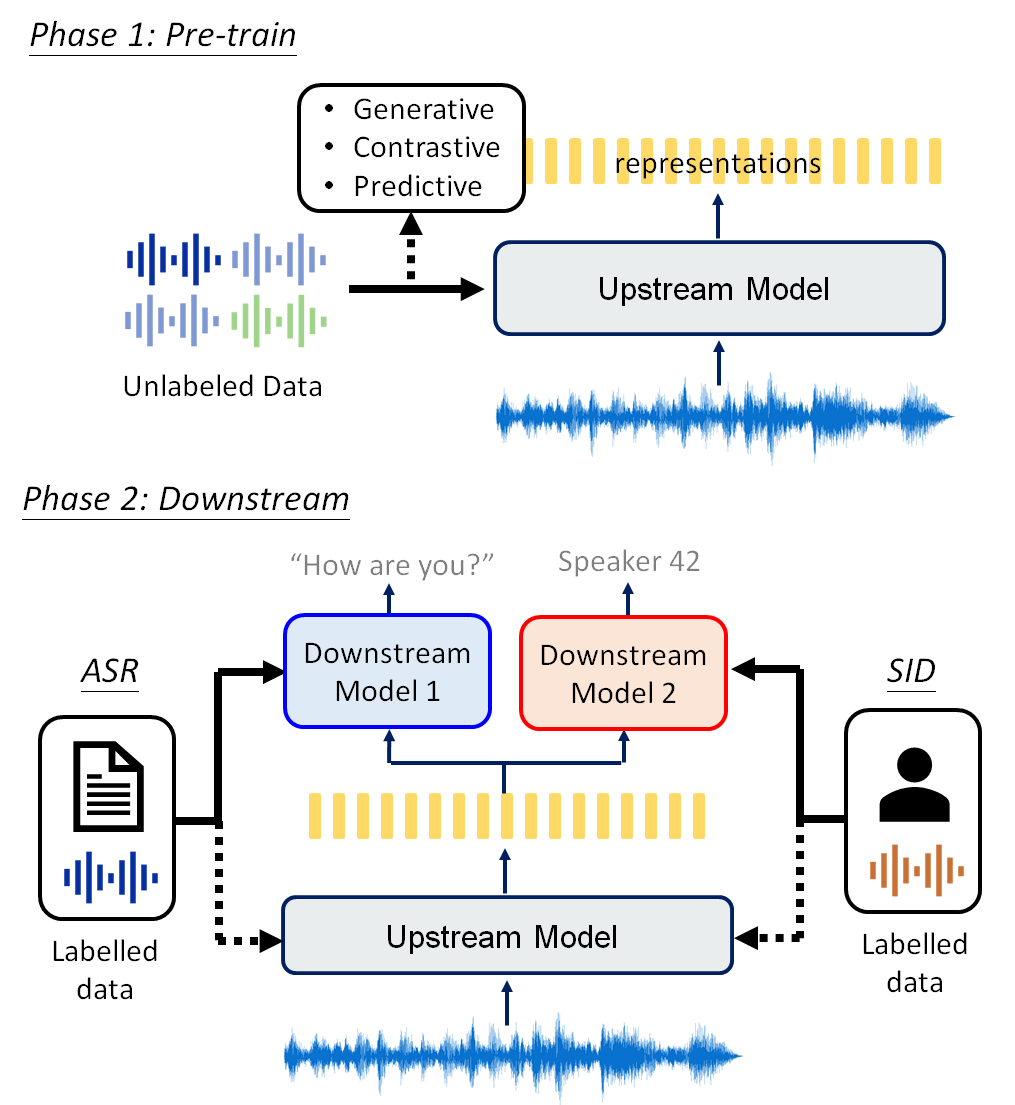
\includegraphics[width=0.80\textwidth]{paper_review/SSL_framework.png}
	 \caption{Framework for using self-supervised representation learning in
	 downstream applications.}
    \label{fig:SSL_framework}
\end{figure}


Over the past decade, deep learning approaches have revolutionized speech processing
through a giant leap in performance, enabling various real-world applications.
Supervised learning of deep neural networks has been the cornerstone of this
transformation, offering impressive gains for scenarios rich in labeled
% data~\cite{lecun_deep_2015}. 
% data~\cite{lecun_deep_2015, hinton_deep_2012}. 
% data~\cite{bourlard_connectionist_1994}. 
% data~\cite{lecun_deep_2015,bourlard_connectionist_1994}. 
data~\cite{lecun_deep_2015,hinton_deep_2012,bourlard_connectionist_1994}. 
Paradoxically, this heavy reliance on supervised learning has restricted progress in
languages and domains that do not attract the same level of labeling
investment. 

To overcome the need for labeled data, researchers have explored approaches that use
unpaired audio-only data to open up new industrial speech use-cases and
low-resource languages~\cite{kemp_unsupervised_1999, lamel_lightly_2002, ma_unsupervised_2006}. Inspired by how
children learn their first language through listening and interacting with
family and surroundings, scientists seek to use raw waveforms and
spectral signals to learn speech representations that capture low-level
acoustic events, lexical knowledge, all the way to syntactic and semantic
information. These learned representations are then used for target downstream
applications requiring a minimal number of labeled data~\cite{hinton_learning_2007,
lecun_tutorial_2006, bengio_representation_2013}. 
Formally, representation learning refers to algorithms for extracting latent
features that capture the underlying explanatory factors for the observed
input~\cite{bengio_representation_2013}. 

Representation learning approaches are generally considered examples of \textit{unsupervised
learning}, which refers to the family of machine learning methods that discover
naturally occurring patterns in training samples for which there are no pre-assigned
labels or scores~\cite{jordan_machine_2015}. 
The term ``unsupervised'' is used to distinguish this family of methods from
``supervised'' approaches, which assign a label to each training sample, and
``semi-supervised'' approaches, which utilize a small number of training samples
with labels to guide learning using a larger volume of unlabeled samples.
Examples of unsupervised learning techniques include $k$-means clustering~\cite{gray_vector_1984}, mixture models~\cite{jordan_hierarchical_1994}, autoencoders~\cite{hinton_autoencoders_1994},
and non-negative matrix factorization~\cite{lee_learning_1999}. 
\textit{Self-supervised learning} (SSL) is a fast-growing subcategory of
unsupervised learning approaches, which are techniques that utilize
information extracted from the input data itself as the label to learn
representations useful for 
downstream tasks. {\color{black} For example, unsupervised $k$-means clustering doesn't adhere to this definition of self-supervision since it iteratively minimizes the within-cluster variance during learning.}
In this review, we
focus on self-supervised learning approaches.

\Cref{fig:SSL_framework} outlines self-supervised representation learning in
relation to downstream applications. 
There are two stages in this framework.
In the first stage, we use SSL to pre-train a \textit{representation model},
also called an \textit{upstream model} or a \textit{foundation model}.
In the second stage, downstream tasks use either the learned
representation from the frozen model, or fine-tune the entire pre-trained model
in a supervised phase~\cite{hinton_reducing_2006}. 
Automatic speech recognition (ASR) and speaker identification (SID) are 
examples of downstream applications in \cref{fig:SSL_framework}.

It is considered desirable for learned speech representations to be
disentangled, invariant, and hierarchical.
Since spoken utterances contain much richer information than the corresponding text
transcriptions---e.g., speaker identity, style, emotion, surrounding noise, and
communication channel noise---it is important to learn representations that
disentangle these factors of variation. Furthermore, invariance of the learned
features to changes in background noise and in the communication channel ensures
stability with respect to downstream application scenarios. Learning feature
hierarchies at the acoustic, lexical, and semantic levels supports applications
with different requirements. For instance, whereas a speaker identification task
benefits from a low-level acoustic representation, a speech
translation task requires a more semantic representation of the input
utterance. 

Due to the popularity of SSL, reviews have been published about the
technology in general~\cite{bommasani_opportunities_2021,ericsson_selfsupervised_2022,liu_selfsupervised_2021} as well as its application to natural language processing (NLP)~\cite{rogers_primer_2020,liu_pretrain_2021,xia_which_2020,qiu_pretrained_2020} and computer vision (CV)~\cite{jing_selfsupervised_2021}. Recently, a brief overview with a general focus on speech representation learning was published \cite{borgholt_brief_2022}. 
However, none of these overviews focus exclusively on SSL for speech processing. Since the speech signal differs greatly from image and text inputs, many  theories  and technologies have been developed to address the unique challenges of speech. 
One review addresses speech representation learning based on deep learning models~\cite{latif_deep_2021}, but does not address recent developments in self-supervised learning. This motivates this overview of speech SSL.


The structure of this paper is arranged as follows. \Cref{sec:thirdwave}
briefly reviews the history of speech representation learning, and
\cref{sec:approach} reviews current speech SSL models.
\Cref{section:benchmark} surveys SSL datasets and benchmarks, 
and discusses and compares results from different works. \Cref{analysis}
analyzes successful SSL approaches and offers insights into the
importance of technological innovations. \Cref{sec:zero} reviews 
zero-resource downstream tasks that utilize SSL. 
Finally, \cref{sec:conclusion} summarizes the paper and suggests 
future research directions.



%!TEX root = ../thesis.tex

\section{Historical Context of Representation Learning}

\label{sec:thirdwave}

In this section we present the historical background of the current surge in
self-supervised representation learning methods in the context of two previous
waves of research work in the 1990s and 2000s. The discussed approaches go
beyond speech to describe the overall landscape of machine learning development during the
past few decades.

\subsection{Clustering and mixture models}

Initial research in learning latent speech and audio representations involved
simple models in which the training data likelihood was optimized directly
or via the expectation--maximization (EM) algorithm.

Early work used simple clustering methods. For example, in work such
as \cite{rabiner_considerations_1979,wilpon_modified_1985}, word patterns were clustered
semi-automatically using techniques such as k-means, after which isolated words
were recognized by finding the training cluster closest to 
  the test data.

Through time, modeling techniques improved such that subword units were
represented by Gaussian mixture models (GMMs) \cite{gauvain_maximum_1994}, which facilitated
the modeling of more variability in the input data. GMMs were first built for
context-independent phonemes; state-clustering 
algorithms~\cite{young_state_1994} then resulted in GMMs for context-dependent phonemes. 
Each latent component of these mixture models acted as a template of a
prototypical speech frame, 
making it difficult to handle 
large volumes of data with diverse characteristics. 
Furthermore, dynamical models like hidden Markov models (HMMs)~\cite{bell_adaptation_2021}
allowed for the processing of continuous speech rather than just isolated word
recognition. These generative GMM and HMM models were trained by maximizing the
likelihood of data given the model, which could be accomplished in either an
unsupervised or a supervised manner.

Another line of research focused on extracting speech features from generative
models. The main objective here was to render the knowledge learned by generative
models accessible to discriminative downstream classifiers, or to map
variable-length sequences to fixed-length representations. Feature vectors
were derived from the parameters of trained GMM models. In the case of {\em
Fisher vectors}, the features were the normalized gradients of the
log-likelihood with respect to the model parameters (mixture weights, means, and
variances) of the Gaussian mixtures. An extension of this approach (likelihood
ratio score space) used the derivative of the log-likelihood ratio of two
models, e.g., a background model and a foreground model. Examples of their use
in speech processing include speech recognition~\cite{smith_speech_2001,venkataramani_support_2003} and
speaker recognition~\cite{wan_svmsvm_2003}. Subsequent techniques in speaker and language
verification~\cite{dehak_frontend_2011,dehak_language_2011} similarly extracted parameters
(concatenated means) from trained background GMMs as representations that were
then combined with low-rank projections of speaker/session- or language-specific
vectors.



\subsection{Stacked neural models}
\label{subsec:stack}

More recently, representation learning has seen a shift of focus towards neural models,
which, compared to GMMs and HMMs, offer distributed representations with more
capacity to model diverse input signals into efficient latent binary codes. 
Examples of early techniques include restricted Boltzmann machines
(RBM)~\cite{hinton_reducing_2006}, denoising autoencoders~\cite{vincent_stacked_2010}, noise contrastive
estimation (NCE)~\cite{gutmann_noisecontrastive_2012}, sparse coding~\cite{olshausen_emergence_1996,
lee_efficient_2006, sivaram_sparse_2010}, and energy-based methods~\cite{ranzato_unified_2007}.
Many of these techniques have also been applied to CV and NLP problems, which
provided inspiration for their application to speech.

Higher-capacity neural models were achieved by stacking several neural network
layers to build progressively higher-level concept representations.
However, these deeper networks also increased the training complexities. For
example, approximate training methods such as contrastive divergence
\cite{hinton_training_2002} were a practical technique to streamline RBM training. 
Furthermore, deep networks had non-convex objective functions, which
often resulted in long training times compared to GMMs, which are trained
using full batches instead of mini-batch learning.

\subsection{Learning through pretext task optimization}

A more recent trend is learning networks that map the input to desired
representations by solving a \textit{pretext} task. Such studies have several
characteristics:
(1)~All layers are trained end-to-end to optimize a single pretext task instead
of relying on layer-wise pre-training
(2)~Past stacked networks typically had only a few layers, but 
very deep networks with more than ten layers are now common.
(3)~It is common to evaluate a representation model on a wide range of tasks.
For example, in NLP, a representation model is usually assessed on GLUE,
which comprises nine tasks~\cite{wang_glue_2018}, whereas in speech, a representation model can be
evaluated on SUPERB, which comprises ten tasks~\cite{yang_superb_2021}, 
as described in detail in \cref{sec:benchmark}.

The cornerstone of this third wave is the design of a pretext task, which
allows the model to efficiently leverage knowledge from unlabeled data.
The pretext task should be challenging enough for the model to learn high-level
abstract representations and 
% not be too amiable to exploit low-level shortcuts.
  not be so easy as to encourage the exploitation of low-level shortcuts.  % AMH: check
Early breakthroughs included end-to-end learning of deep neural architectures
via pretext tasks for restoring the true color of black-and-white
images~\cite{zhang_colorful_2016}, joint learning of latent representations and their
cluster assignments~\cite{caron_deep_2018}, and the prediction of the relative positions of
image patches~\cite{doersch_unsupervised_2016}. Other popular approaches include variational
autoencoders (VAEs)~\cite{kingma_autoencoding_2014, rezende_stochastic_2014}. While typical autoencoders learn data
representations using unsupervised objectives by reconstructing the input
after passing it through an information bottleneck, VAEs estimate a neural model of a probability density function (pdf) that approximates the unknown “true” distribution of the observed data, for which we only have access to independently identically distributed (iid) samples. It is also important to mention dynamical VAEs \cite{girin_dynamical_2021}, which is an extension of VAE for sequential data such as speech.

In the SSL context, a pretext task related to autoencoding is to generate
an object from its partial information. Such tasks are widely used in NLP, for
example, using 
the previous tokens 
in a sentence to predict the next token such as in
ELMo~\cite{peters_deep_2018}, the GPT
series~\cite{radford_language_2019}, and 
Megatron~\cite{shoeybi_megatronlm_2020}, or predicting the masked tokens in a
sentence such as with the bidirectional encoder representations from Transformers
(BERT) series~\cite{devlin_bert:_2018,liu_roberta_2019}. 
Another common pretext task in the third wave is contrastive
learning~\cite{oord_representation_2018}, in which a model learns to identify a
target instance from a set of negative samples. 
This approach has become especially popular in the
CV context~\cite{chen_simple_2020,he_momentum_2020,chen_improved_2020,caron_unsupervised_2020}.
In this survey, we will mainly focus on techniques for pretext task
optimization for speech processing, and discuss these techniques in detail
in \cref{sec:approach}.


\subsection{Other related work}
A closely related area of research that is not covered in this review is
semi-supervised pre-training methods such as pseudo-labeling (that is,
self-training). Pseudo-labeling (PL) relies on a supervised teacher model to
label a large volume of speech-only data, which is then used to augment the
initial labeled data to train a student model~\cite{kemp_unsupervised_1999, lamel_lightly_2002,
ma_unsupervised_2006, parthasarathi_lessons_2019}. PL has been successful and widely adopted in the
speech community since the 1990s. Other proposed variations of PL include
augmenting speech-only data with noise to improve robustness, iterating
over the PL process to improve teacher labeling quality, and training student
models with more parameters than their original teachers to capture the
complexities in vastly larger speech-only data~\cite{park_improved_2020,
xu_iterative_2020, xiao_scaling_2021}. 
Both SSL and PL leverage unlabeled speech-only data.
One distinguishing factor in PL is the utilization of supervised data for a
specific task during model pre-training, which limits the model's focus to
a single (or at best a few) downstream tasks. 
SSL, in turn, is an attempt to learn task-agnostic representations to benefit
a wide range of tasks. 

Transfer learning (TL) is another closely related area of research for
pre-training speech models. TL transfers knowledge captured by models
trained on one task to different but related tasks~\cite{caruana_multitask_1997}. 
The past few decades have seen active research on TL and its
extension to multitask learning for more general representations. 
Multilingual and cross-lingual supervised models have proven superior in
low-resource speech recognition tasks~\cite{cui_multilingual_2015}.
SSL can be regarded as a type of TL because knowledge learned from pre-training
is used for different downstream tasks.
This survey paper focuses on SSL, and not all TL technologies for speech. 
One survey indeed addresses TL for speech processing~\cite{bell_adaptation_2021}
but does not include current SSL technologies for speech.  

%!TEX root = ../thesis.tex

\section{Speech representation learning paradigms} \label{sec:approach}
Due to the characteristics of speech, SSL pretext tasks developed for CV
and NLP may not directly apply to speech.
Below we summarize the characteristics of speech as compared to CV and NLP.
\begin{itemize}
\item \textit{Speech is a sequence.} 
Unlike CV, in which an image usually has a fixed size representation, it is
natural to represent a speech utterance as a variable-length sequence. 
Therefore, pretext tasks developed for CV cannot generally be directly
applied to speech.

\item \textit{Speech is a long sequence without segment boundaries.} 
Both text and speech can be represented as sequences. From this viewpoint, it
is natural to apply learning approaches developed for text directly to
speech. 
In NLP, morpheme-like tokens are widely used as sequence units in
pre-training. The standard BERT takes 512 morpheme-like tokens as
input, usually covering a paragraph including several sentences. 
However, speech signals consist of sound pressure measurements with thousands
of samples per second, resulting in sequences much longer than those for text. Even
spectral representations which reduce the sequence length can have hundreds of
frames per second.
Processing such sequences with typical neural network architectures like
Transformers can result in problems with running time and memory requirements. 
One could gather consecutive frames to form shorter segments,
but unlike text, there is no obvious segmentation for unlabeled
speech.
\item \textit{Speech is continuous.} 
In NLP, it is common to use a pretext task that models a categorical
distribution of masked or future inputs. Since text is easily broken down into
individual tokens such as words, subwords, or characters, it is
straightforward to define a finite vocabulary for such tasks.
However, this idea does not apply to speech modeling because speech
signals are continuous; 
in this sense there is no such thing as a speech vocabulary. 
\item \textit{Speech processing tasks are diverse.}
Building generalizable self-supervised representation models for diverse speech
processing tasks is challenging.
Speech contains rich, hierarchical information, and different speech tasks
may require mutually orthogonal information.
For example, speech recognition requires a model that extracts content information
but ignores speaker information; in contrast, speaker recognition 
requires a model that extracts speaker information but removes content information.
Therefore, it is challenging to define a self-supervised model whose
representations are suitable for both speech recognition and speaker
recognition. Analogous considerations apply within CV and NLP.
\end{itemize}

In the sections below, we group modern SSL pretext tasks designed for speech
into three main categories: \textit{generative} approaches,
\textit{contrastive} approaches and \textit{predictive} approaches. 
\Cref{fig:timeline} shows a timeline of the models covered in these sections
with each model colored according to our categorization. 
\Cref{table:pretext} summarizes model pretext tasks along within the categories.


\subsection{Notation}
\label{sec:notation}

To efficiently describe the different approaches, we use a simple
notation. Models are assumed to consist of functions $f(\cdot)$ and $g(\cdot)$, where $f(\cdot)$  denotes the representation model to be used after pre-training and $g(\cdot)$ is an auxiliary module needed only to support the pretext task. For instance, in a classic autoencoder, $f(\cdot)$ would denote the encoder and $g(\cdot)$ the decoder. For more complex models, these functions might consist of several components indicated by sub-indices $f_1(\cdot) \dots f_N(\cdot)$. As we will see, many self-supervised models use masking, which replaces some parts of the input or a hidden representation  by zeros or a learned vector. We use $m(\cdot)$ to denote a function that applies such masking to its input. Similar to $g(\cdot)$, this function is only used during pre-training. 

Given an acoustic input $X =\{x_1,x_2, ..., x_T\}$, $f(\cdot)$ outputs a representation $H =\{h_1,h_2,...,h_T\}$. The input~$X$ may be either the raw waveform samples or a sequence of spectral feature vectors. Both are viable options in practice. For simplicity, we do not distinguish between the two in our notation.  

While $f(\cdot)$ always takes an acoustic input, the input to $g(\cdot)$ can be either the acoustic signal or another learned representation. Most importantly, $g(\cdot)$ produces an output that is used for the pretext task but is not  used by $f(\cdot)$ to produce the representation $H$. Hence, $g(\cdot)$ can be discarded after pre-training. Finally, $f(\cdot)$ commonly downsamples the temporal dimension, but again, this is not crucial to understand the models, so consider only a single temporal scale $t\in\{1,\dots, T\}$ for notational convenience.

We use $Q = \{q_1,q_2, ..., q_T\}$ to denote representations that are quantized via codebook learning. Alternatively, discrete representations may take the form of one-hot vectors, or the equivalent integer IDs, which we denote by $C = \{c_1,c_2, ..., c_T\}$. We use a circumflex to denote that, for instance, $\hat{x}_t$ is an approximation of $x_t$. Finally, we often use a subscript when defining a loss, $\mathcal{L}_i$, to imply that the total loss is computed as a sum over $i$, unless otherwise stated.

For some models, we will refer to $H$ as a \emph{contextualized} representation which means that each $h_t$ is a function of some, linguistically speaking, long sub-sequence of $X$ spanning at least several phonemes. Usually, $h_t$ depends on the entire input $X$ or all previous timesteps $X_{[1,t]}$. In contrast, a \emph{localized} representation is one that only depends on a short part of the input $X_{[t - u,t + u]}$, where $u \geq 0$. The distinction between contextualized and localized may become fuzzy if $u$ is large, however, this is rarely the case.

\edit{After pre-training,} the representation model $f(\cdot)$ can be fine-tuned for a downstream task directly or used to extract features which are fed to another model, as visualized in \cref{fig:SSL_framework}. It is not uncommon to use the output representation~$H$, but often representations from hidden layers of $f(\cdot)$ are better suited \parencite{pasad_layerwise_2021}.


\begin{figure*}[t]
    \centering
    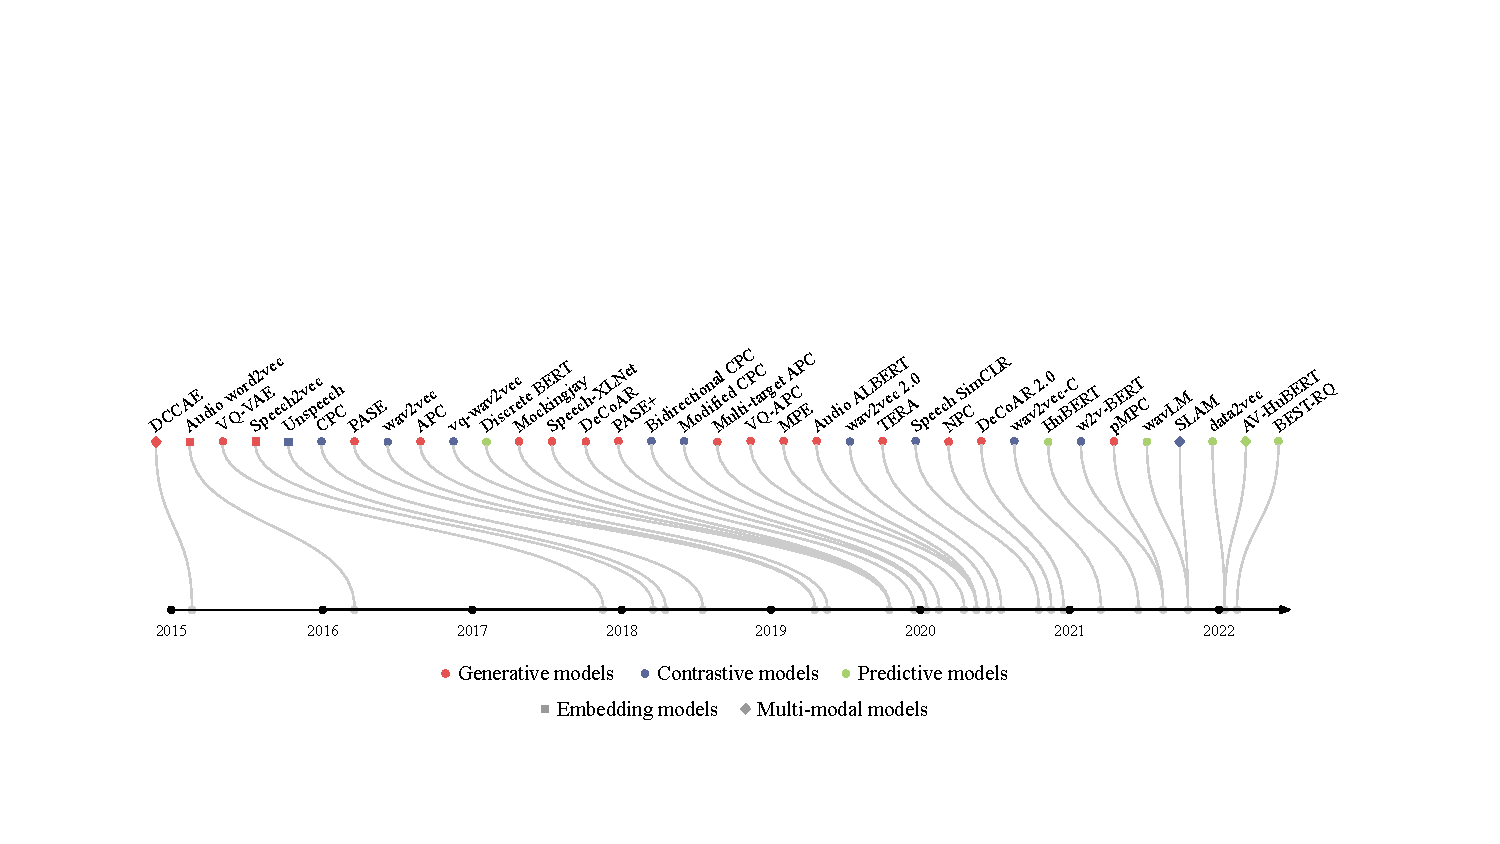
\includegraphics[width=0.98\textwidth]{paper_review/model_timeline.pdf}
   % \includegraphics[width=0.98\textwidth]{paper_review/model_timeline_wo_dccae.pdf}
	 \caption[Selection of self-supervised models for speech.]{A selection of models listed according to first publication date
	 on arXiv or conference submission date when this clearly precedes the
	 former. The models are categorized as generative, contrastive, or predictive.
	 In addition, some models are characterized as embedding models or
	 multi-modal models, although most learn frame-level
	 representations from speech only. Some models use a mixture of generative
	 and contrastive tasks. For instance, PASE and PASE+ use a multi-task setup,
	 but find that generative tasks are the most important for downstream
	 task performance~\parencite{pascual_learning_2019}.}
    \label{fig:timeline}
\end{figure*}


 

\subsection{Generative approaches}
\label{sec:generative}

\subsubsection{Motivation}

In this category, the pretext task is to generate, or reconstruct, the input data based on some limited view. This includes predicting future inputs from past inputs, masked from unmasked, or the original from some other corrupted view.  ``Generative'' as used in this paper hence refers to models that target the original input in their pretext task. Note that this differs from generative models, which learn \ci{distributions that allow} to sample new data.

\subsubsection{Approaches}

\paragraph{Autoencoding} 
Since their introduction in the mid-1990s~\parencite{hinton_autoencoders_1994}, autoencoders (AEs)
have played an essential role in learning distributed latent representations of
sensory data. 
As described above, AEs consist of an encoder and decoder; the pretext task
is to reconstruct the given input. The most common type of AE places an
information bottleneck on the latent representation by simply having fewer
hidden units available than input features. This forces the model to discard
low-level details and disccourages the learning of trivial solutions. Other models add
regularization to the latent space to further improve the quality of the
learned representations.
For instance, denoising autoencoders (DAEs) learn latent representations by
reconstructing from input corrupted by noise~\parencite{vincent_stacked_2010}. 
\edit{The Variational Autoencoder (VAE) is a probabilistic version of the AE which defines the latent representation via a posterior distribution over stochastic latent variables \parencite{kingma_autoencoding_2014,rezende_stochastic_2014}. VAEs have been applied to speech in numerous works \parencite{chung_recurrent_2015, fraccaro_sequential_2016, hsu_learning_2017, hsu_unsupervised_2017, aksan_stcn_2019}}.
The vector-quantized variational autoencoder (VQ-VAE) is another model in this
category~\parencite{oord_neural_2018};
it extends the original VAE~\parencite{kingma_autoencoding_2014} with a novel
parameterization of the posterior distribution for discrete latent
representations. 
\edit{The VQ-VAE has been instrumental in generative speech modelling and recent work on generative spoken language modeling has successfully combined the idea of a discrete latent space with self-supervised learning \parencite{polyak_speech_2021, kharitonov_textfree_2021, nguyen_generative_2022}.}



Specifically, in the VQ-VAE, the continuous representation vector $h_t$ at the output of the encoder is quantized by mapping it to a codebook vector, which is then used as the input to the decoder. This operation is non-differentiable and the \edit{gradients of the loss with respect to the encoder parameters} must be obtained by approximation. In the VQ-VAE this is done using the straight-through estimator~\parencite{bengio_estimating_2013}, i.e., the gradients \edit{with respect to the} encoder output are taken to be equal to those \edit{with respect to the} decoder input \ci{(i.e., the quatization step is ignored)}. Given a learned codebook $A\in\mathbb{R}^{K \times D}$, where $K$ is the codebook size and $D$ is the dimensionality of each codebook vector $a_k$, the quantized representation $q_t$ of $h_t$ is obtained as
\begin{align}
    q_t = a_k, \text{ where } k=\arg\min_j \norm{h_t - a_j}_2 \enspace .
\end{align}
\edit{The decoder $g(\cdot)$ is an autoregressive model that takes $q_{[1,t]}$ as input to generate $x_t$ \parencite{oord_wavenet_2016}}. 
Codebook learning is facilitated by a two-term auxiliary loss similar to
classical vector quantization dictionary 
learning~\parencite{burton_generalization_1983, soong_vector_1985}. 
Gradients for the codebook vectors are given solely by a term that moves
codebook vectors $a_k$ closer to the non-quantized vectors $h_t$. A so-called
\emph{commitment term} is added to ensure that non-quantized vectors do not grow
unboundedly by enforcing the encoder to keep them close to a codebook vector.
This commitment term is optimized only by the encoder. The
total VQ-VAE loss for a single timestep is

\begin{align}
    \mathcal{L}_t = \underset{\text{encoder+decoder}}{\underbrace{\log p(x_t | q_{[1,t]})}}
     + \underset{\text{codebook}}{\underbrace{\text{MSE}\left(\mathrm{sg}\left[h_t\right], A\right)}}
     + \underset{\text{encoder}}{\underbrace{\alpha~\text{MSE}\left(h_t, \mathrm{sg}\left[A\right]\right)}} \enspace ,
    \label{eq: vector quantization losses}
\end{align}%
\noindent where \edit{$\log p(x_t|q_{[1,t]})$ is a reconstruction likelihood term usually using a categorical distribution,} $\mathrm{sg}[x] = x$ is the so-called stop-gradient operator \edit{which acts as the identity function during the forward pass but \ci{is assumed to have}
partial derivatives all equal to zero during the backward pass}, $\alpha$ is a scalar hyperparameter, 
\edit{and we define $\text{MSE}(h_t,A) = \frac{1}{KD} \sum_{k=1}^{K}\sum_{i=1}^{D}\left(h_{t,i} - a_{k,i}\right)^2$. 
The loss for a full sequence is the sum or mean over all $\mathcal{L}_t$.} 

These learned discrete representations have been shown to capture high-level
speech information closely related to phonemes, and are useful for
applications such as speaker conversion~\parencite{chorowski_unsupervised_2019}.
Vector quantization is \edit{not} exclusive to VQ-VAE but has seen
widespread application within SSL for regularization purposes and to define
targets for the pretext task. We will cover these applications below.

\edit{The Gumbel softmax \parencite{jang_categorical_2016} is another frequently used approach for obtaining a discrete representation space, and has also been used for AEs \parencite{eloff_unsupervised_2019}. In addition to the approaches discussed above, several other works on speech representation learning take inspiration from the AE framework \parencite{zeiler_rectified_2013, badino_autoencoder_2014, badino_discovering_2015, kamper_unsupervised_2015, renshaw_comparison_2015, settle_acoustically_2019}.}


\begin{comment}
\paragraph{Regularization}
In the generative-based approaches, some regularization in the encoder $f(\cdot)$ or decoder $g(\cdot)$ is required to encourage the model to utilize global speech information and prevent naive copying input when reconstruction. 
The models below have been enhanced by regularization methods. 
\begin{itemize}
%\item VAE, VQ-VAE
    \item DeCoAR 2.0~\parencite{ling_decoar_2020} presents a deep contextualized acoustic representation learning approach with the addition of a vector quantization (VQ) layer.
    \item In VQ-APC~\parencite{chung_vectorquantized_2020}, a VQ layer is used with the APC objective, which imposes a bottleneck and forces the model to learn better representations.
    \item Two dropout regularization methods, attention dropout and layer dropout, are introduced to TERA~\parencite{luo_dropout_2021}. 
\end{itemize}
\end{comment}

\paragraph{Autoregressive prediction}
\label{par:apc}

Autoregressive predictive coding (APC)~\parencite{chung_unsupervised_2019,
chung_generative_2020} \edit{takes inspiration from the classic Linear Predictive Coding (LPC) approach for speech feature extraction~\parencite{oshaughnessy_linear_1988} and autoregressive language models (LM) for text, where the model learns to predict future information from past}.
\edit{A function} $f(\cdot)$ reads the input sequence $X_{[1,t]}$ and \edit{outputs a representation sequence} $H_{[1,t]}$.
The \edit{auxiliary module} $g(\cdot)$ is a linear projection layer which takes the last vector of $H_{[1,t]}$ as input to \edit{approximate} $x_{t+c}$, where $c \geq 1$. Thus, $c$ indicates how many timesteps the model predicts ahead. The \edit{modules} $f(\cdot)$
and $g(\cdot)$ are jointly learned to minimize {the \ensuremath{L_1} loss between $x_{t+c}$ and its approximation $\hat{x}_{t+c}$}. APC is formulated as 
\begin{align}
    H_{[1,t]} &= f(X_{[1,t]}) , \\
    \hat{x}_{t+c} &= g(h_{t}) \label{eq:c} , \\
    \mathcal{L}_t &= \lVert \hat{x}_{t+c} - x_{t+c} \rVert_1 \enspace .
\end{align}
In text-based autoregressive LMs, $c$ is set to $1$ \edit{to enable autoregressive generation}. However, due to the smoothness of the speech signal, neighboring acoustic features are usually similar. Depending on the downstream task, we are often interested in learning so-called \emph{slow features} that typically span multiple input frames~\parencite{wiskott_slow_2002}. Even the smallest linguistic units of speech---phonemes---span $0.07$~seconds on average in the English TIMIT dataset~\parencite{garofolo_timit_1993},   whereas spectrogram frames $\mathbf{x}_t$ are typically computed at $0.01$ second intervals. Thus, simply predicting the next frame constitutes a trivial pretext task for APC; the original work finds that $c=3$ performs well. 
In \parencite{chung_improved_2020}, the APC objective is extended to multi-target
training. The new objective generates both past and future frames conditioned
on previous context. 
In VQ-APC~\parencite{chung_vectorquantized_2020}, quantization is used with the APC
objective, which imposes an information bottleneck serving as a regularizer.

A drawback of APC is that it encodes information only from previous timesteps
and not the entire input.
DeCoAR~\parencite{ling_deep_2020} combines the bidirectionality of the popular NLP model
ELMo~\parencite{peters_deep_2018} and the reconstruction objective of APC to alleviate
this issue and allow encoding information from the entire input. 
It uses a forward LSTM $f_1(\cdot)$ to encode $X_{[1,t]}$ and a backward LSTM
$f_2(\cdot)$ to encode $X_{[t+k,T]}$, where $k>1$: 
\begin{gather}
    H_{[1,t]} = f_1(X_{[1,t]}), \\
    H^\prime_{[t+k,T]} = f_2(X_{[t+k,T]}), \\
    \hat{X}_{[t+1,t+k-1]} = g(h_t, h^\prime_{t+k}) \enspace .
\end{gather}
The input feature vector used in the downstream tasks is the concatenation of
$h_{t}$ and $h^\prime_{t}$. 


\paragraph{Masked reconstruction}

Masked reconstruction is largely inspired by the masked language model (MLM) task from BERT~\parencite{devlin_bert_2018}. During BERT pre-training, some tokens in the input sentences are masked by randomly replacing them by a learned masking token or another input token. The model learns to reconstruct the masked tokens from the non-masked tokens. Recent work has explored similar pretext tasks \edit{for speech representation learning}. Similar to the DeCoAR model described above, this allows a model to learn contextualized representations that encode information from the entire input. While we here focus on the models that reconstruct the masked input, it is important to note that masking has also been used extensively for contrastive (\cref{contrastive_approaches}) and predictive (\cref{predictive_approaches}) models. 

From a high-level perspective, the training phase of models using masked
reconstruction can be formulated as
\begin{align}
    H &= f(m(X)), \\
    \hat{x}_t &= g(h_{t}), \\
    \mathcal{L}_t &= \lVert \hat{x}_{t} - x_{t} \rVert_1 .
\end{align}
\edit{The exact masking policy defined by $m(\cdot)$ differs from model to model and will be discussed further below.}
The function $f(\cdot)$ is typically a Transformer encoder~\parencite{liu_mockingjay_2020,jiang_improving_2019,liu_masked_2020}, but recurrent neural networks have also been used~\parencite{wang_unsupervised_2020}. \edit{In general, the Transformer encoder architecture has been adopted widely by self-supervised models for speech within all three surveyed categories.} \edit{The function $g(\cdot)$ is usually a linear projection or a multilayer perceptron (MLP)}. Finally, the loss $\mathcal{L}_t$ is commonly computed only for masked timesteps in order to discourage the model from learning an identity mapping.

The masking policies used in NLP can be adapted to speech by considering a speech \edit{segment} equivalent to a token in a sentence; indeed, the masking strategy of BERT has also been used for speech pre-training~\parencite{liu_mockingjay_2020}.
In the standard BERT masking policy, each token is masked independently at random. However, for speech, masking a single \edit{sample or spectrogram frame results in a largely} trivial reconstruction task \edit{since, as discussed in \cref{par:apc}, the smoothness of audio signals may encourage the model to learn to simply interpolate neighboring frames.} Therefore it is common to mask chunks of consecutive frames~\parencite{liu_mockingjay_2020,jiang_further_2021}. 

We can bring the pretext task closer to the NLP equivalent by using a masking policy where the masked regions of the input correspond to linguistic units. Instead of just masking a fixed number of consecutive frames, pMPC~\parencite{yue_phonetically_2021} selects masked speech frames according to the phonetic segmentation in an utterance. \edit{However, in order to obtain this segmentation, some labeled data is of course needed.}

Whereas most studies use masking along the temporal dimension of the input, speech can also be masked along the frequency dimension when spectral input features are used~\parencite{wang_unsupervised_2020,liu_tera_2021}. Frequency masking has been shown to improve representations used for speaker classification~\parencite{liu_tera_2021}. 

Some studies explore alternatives to masking the input directly. In non-autoregressive predictive coding (NPC)~\parencite{liu_nonautoregressive_2020}, time masking is introduced through masked convolution blocks. Taking inspiration from XLNet~\parencite{yang_xlnet_2019}, it has also been suggested that the input be reconstructed from a shuffled version~\parencite{song_speechxlnet_2020} to address the discrepancy between pre-training and fine-tuning of masking-based approaches.

Regularization methods can further improve on masked reconstruction approaches. \edit{DeCoAR 2.0~\parencite{ling_decoar_2020} uses vector quantization}, which is shown to improve the learned representations. Furthermore, two dropout regularization methods---attention dropout and layer dropout---are introduced with the TERA model~\parencite{liu_tera_2021, luo_dropout_2021}. \edit{Both methods are variations on the original dropout method \parencite{srivastava_dropout_2014}.}

\paragraph{More generative approaches}
Other than the autoregressive and masked reconstruction tasks discussed above, various studies have explored the reconstruction of other targets derived from the input. PASE and PASE+~\parencite{pascual_learning_2019,ravanelli_multitask_2020} use multiple targets, including the waveform, log power spectrum, \edit{mel cepstral coefficients (MFCCs)}, and prosody features. Models that learn acoustic embeddings of small speech segments have targeted future and past spectrogram segments~\parencite{chung_speech2vec_2018, tagliasacchi_selfsupervised_2019, tagliasacchi_pretraining_2020}, phase information~\parencite{quitry_learning_2019}, and the temporal gap between two segments~\parencite{tagliasacchi_selfsupervised_2019, tagliasacchi_pretraining_2020}.


\subsubsection{Challenges} 

Although successful NLP models like BERT and GPT are based on generative pretext tasks, the progress have not been translated directly to the speech domain. A speech signal encodes more information than text, such as speaker identity and prosodic features, which makes it harder to generate. However, in order to generate all details of the input, the model must encode all information in the speech signal. Hence, a model that learns to perfectly reconstruct its input may not necessarily have learned to isolate the features of interest \edit{\ci{and will encode} redundant information for a given downstream task.} 

There are many choices involved in designing a generative pretext task. For instance, \edit{masking strategy and the choice of input and target representation (e.g., waveform samples or spectral
features)}. These choices influence what the model learns through the pretext task. However, there is little research on the relationship between task design and the information encoded in the learned representations.

%!TEX root = ../thesis.tex

\begin{table*}[!htb]
    \centering
    \caption{
    A summary of the approaches in the three categories of
    self-supervised learning. 
    Column~(a) lists the names of the models and related references, 
    column~(b) defines the model input, 
    column~(c) defines any corruption of the input or hidden representation, and
    column~(d) defines the target of the pretext task; the pretext task itself
    is described by the overall model category and the main text.
    $X=\{x_1,x_2,...,x_T\}$ is the input sequence in which $x_t$ can be an
    acoustic feature vector (e.g., MFCC, filterbank, or spectrogram features)
    or a waveform sample. 
    $X_{[t_1:t_2]}$ represents $\{x_{t_1},x_{t_1+1},...,x_{t_2}\}$.
    $X_{-[t_1:t_2]}$ represents $X$ in which the segment
    $X_{[t_1:t_2]}=\{x_{t_1},x_{t_1+1},...,x_{t_2}\}$ is masked.
    $x_{t}^{i}$ represents the $i$-th dimension of $x_t$.
    If $x_t$ is a frame in a spectrogram, then the $i$-th dimension corresponds
    to a specific frequency bin.
    $X^{-[f,f+j]}$ refers to a spectrogram $X$ which is masked along the frequency
    axis from the $f$-th to $(f+j)$-th bin. 
    % $X_{-[t:t+k]}^{-[f,f+j]}$ refers to a spectrogram $X$ but masked along both time and frequency dimensions. 
    % $X^*$ is a temporally permuted version of $X$, that is, the $x_t$ are randomly shuffled to form $X^*$. 
    We indicate random temporal permutation of a sequence by indexing it with
    the set $\mathcal{P}_t\triangleq\textsc{permute}([0,t])$, where
    $\textsc{permute}(\cdot)$ returns a permutation of the given list. 
    We indicate data augmentation (e.g., reverberation) by the function
    $\textsc{augment}(\cdot)$. Subscripts indicate different augmentations. 
    % $X^\prime$ is an augmented version of $X$ (e.g., $X$ with reverberation), while $X^{\prime\prime}$ is $X$ adding distortion different from  $X^\prime$.
    $Z$ represents a localized latent representation sequence of $X$. %, and $Z^\prime$ and $Z^{\prime\prime}$ are the latent representation sequences of  $X^\prime$ and $X^{\prime\prime}$, respectively. 
    % $Z$ represents a localized latent representation sequence and $Z^\prime$ is the latent representation sequence of $X^\prime$. 
    $Z^{(l)}$ is $Z$ at the $l$-th layer of the model used to compute it.
    $\bar{H}$ is the contextualized sequence $H$ obtained from an exponential
    moving average (EMA) of the model undergoing training with no masking
    applied.
    $Q$ represents a sequence of quantized learned representations, and $C$ is
    a sequence of discrete cluster IDs.
    For contrastive models, we specify only positive targets.
    }
    % \begin{minipage}{\textwidth}  
\centering
\renewcommand*\arraystretch{1.2}{
\begin{tabular}{l|c|c|c}
    \toprule
    \textbf{Model} (a) & \textbf{Input} (b) & \textbf{Corruption} (c) & \textbf{Target} (d) \\
    \midrule
    \midrule
    \multicolumn{4}{c}{\textsc{Generative models}} \\
    \midrule
    \midrule
    Audio Word2vec~\cite{chung_audio_2016}, VQ-VAE~\cite{oord_neural_2018}     & $X$ &   \textsc{-}    &  $X$  \\ %It has VQ as extra constraint.
    \midrule  
    Speech2Vec~\cite{chung_speech2vec_2018}, Audio2Vec~\cite{tagliasacchi_pre_2020} - skip-gram    & $X_{[t_1,t_2]}$  &     \textsc{-}   &    $X_{[t_0,t_1]}$,$X_{[t_2,t_3]}$     \\
    \midrule 
    Speech2Vec~\cite{chung_speech2vec_2018}, Audio2Vec~\cite{tagliasacchi_pre_2020} - cbow    & $X_{[t_0,t_1]}$,$X_{[t_2,t_3]}$   &     \textsc{-}   &    $X_{[t_1,t_2]}$   \\
    \midrule 
    PASE~\cite{pascual_learning_2019}, PASE+~\cite{ravanelli_multi_2020}\footnote{PASE uses multiple pretext tasks, but the authors find that reconstruction is most important.}       & $X$ &  \textsc{-}   &  Different modalities of $X$  \\
    \midrule 
    APC~\cite{chung_unsupervised_2019,chung_vector-quantized_2020}         & $X_{[1,t]}$   & \textsc{-}              & $x_{t+c},\, c\geq1$    \\ %VQ-APC is the same as APC
    \midrule
    Speech-XLNet \cite{song20d_interspeech}     & \multicolumn{2}{c|}{$X_{\mathcal{P}_{t}}$}   &     $x_{i\sim\mathcal{P}^c_{t}}$  \\ %Lee: Use * to represent the permutation, hope it is not strange.
    \midrule  
    DeCoAR~\cite{ling2020deep}     & $X_{[1,t-1]}, X_{[t+k+1,T]}$ & \textsc{-} & $X_{[t,t+k]}$   \\
    \midrule
    Mockingjay~\cite{liu_mockingjay_2020}, Audio ALBERT~\cite{chi2020audio}, DeCoAR 2.0~\cite{ling2020decoar}   & \multicolumn{2}{c|}{$X_{-[t,t+k]}$}   & $X_{[t,t+k]}$    \\
    \midrule 
    TERA~\cite{liu_tera_2021}, BMR~\cite{wang_unsupervised_2020}  & \multicolumn{2}{c|}{$X_{-[t,t+k]}^{-[f,f+j]}$}       & $X$       \\
    \midrule
    pMPC~\cite{yue_pmpc_2021}      &  \multicolumn{2}{c|}{$X_{-[t,t+k^\prime]}$ ($X_{[t,t+k^\prime]}$ is a phoneme)}       & $X_{[t,t+k^\prime]}$    \\
    \midrule 
    MPE~\cite{liu2020masked} & $X$ &  $Z_{-[t,t+k]}$  & $Z$    \\ %Lee: What is the difference between MPE and NPC??? And I believe it reconstruct the convolutional blocks output (learned target?)
    \midrule
    NPC~\cite{liu21l_interspeech}      & $X$  &   $Z_{-[t,t+k]}$  &    $X$   \\ %Lee: I am not 100% sure it is correct. Please check.
    \midrule
    \midrule
    \multicolumn{4}{c}{\textsc{Contrastive models}} \\
    \midrule
    \midrule
    Unspeech \cite{milde2018unspeech}       &   $X_{[t_1,t_2]}$ &   \textsc{-}   &  $X_{[t_0,t_1]}$,$X_{[t_2,t_3]}$ \\
    \midrule 
    CPC~\cite{oord_representation_2018}, wav2vec \cite{schneider_wav2vec:_2019}, Modified CPC \cite{riviere2020unsupervised}         & $X_{[1,t]}$   &    \textsc{-}           & $z_{t+c},\, c\geq1$   \\ %Modified CPC is the same as CPC
    \midrule 
    Bidirectional CPC \cite{kawakami2020learning}      & $X_{[1,t]}$ or $X_{[t,T]}$ &  \textsc{-}    &    $z_{t+c}$ or $z_{t-c},\, c\geq1$   \\
    \midrule 
    vq-wav2vec \cite{baevski_vq-wav2vec_2020}     &   $X_{[1,t]}$ &   \textsc{-}    &   $q_{t+c},\, c\geq1$   \\ 
    \midrule 
    wav2vec 2.0 \cite{baevski2020wav2vec}, wav2vec-C \cite{sadhu_wav2vec-c_2021}\footnote{wav2vec-C adds reconstruction loss to wav2vec 2.0.}    & $X$             & $Z_{-[t,t+k]}$          & $Q_{[t,t+k]}$ \\
    \midrule 
    w2v-BERT \cite{chung_w2vbert_2021}     &$X$ &    $Z_{-[t,t+k]}$   &     $Q_{[t,t+k]}$ and $C_{[t,t+k]}$     \\
    \midrule
    Speech SimCLR \cite{SpeechSimCLR}\footnote{Speech SimCLR targets the latent representation of an augmented version of $X$ using a differently augmented $X$, and vice-versa.}    & \multicolumn{2}{c|}{$\textsc{augment}_1(X)$ and $\textsc{augment}_2(X)$}     &    $\textsc{augment}_2(Z)$ and $\textsc{augment}_1(Z)$   \\ 
    \midrule
    \midrule 
    \multicolumn{4}{c}{\textsc{Predictive models}} \\
    \midrule
    \midrule
    Discrete BERT~\cite{baevski_vq-wav2vec_2020,baevski_effectiveness_2020} \footnote{Discrete BERT obtains codes $C$ from vq-wav2vec.}      &   \multicolumn{2}{c|}{$C_{-[t,t+k]}$}   & $C_{[t,t+k]}$  \\
    \midrule 
    HuBERT \cite{hsu_hubert_2021}\footnote{HuBERT is trained first using cluster IDs of the MFCCs as target and subsequently clusters IDs of the model representations from the last iteration.}, WavLM \cite{chen_wavlm_2021}\footnote{WavLM simulates noisy/overlapped speech as inputs.}  & $X$             & $Z_{-[t,t+k]}$          & $C_{[t,t+k]}$  \\ 
    \midrule
    data2vec \cite{baevski_data2vec_2022}    & $X$             & $Z_{-[t,t+k]}$          & $\sum_{l}\bar{H}^{(l)}_{[t,t+k]}$  \\ 
    \midrule 
    BEST-RQ \cite{BEST-RQ}\footnote{BEST-RQ obtains codes $C$ by quantizing acoustic features using a random projection quantizer.}     &  \multicolumn{2}{c|}{$X_{-[t,t+k]}$}      &  $C_{[t,t+k]}$   \\ 
    \midrule 
    \bottomrule
\end{tabular}
}
    
% \end{minipage}
\label{table:pretext}
\end{table*}


\begin{comment}
\begin{table*}[ht!]
    \centering
    \caption{
    This table summarizes the approaches of the three categories of self-supervised learning. 
    Column (a) lists the names of the models and related references. 
    Column (b) defines the input to the models. 
    Column (c) defines any corruption of the input or some hidden representation. 
    Column (d) defines the target of the pretext task; the pretext task itself is described by the overall model category and the main text.
    $X=\{x_1,x_2,...,x_T\}$ is the input sequence in which $x_t$ can be an acoustic feature vector (e.g., MFCC, filterbank, or spectrogram features) or a waveform sample. 
    $X_{[t_1:t_2]}$ represents $\{x_{t_1},x_{t_1+1},...,x_{t_2}\}$.
    $X_{-[t_1:t_2]}$ represents $X$ with the segment $X_{[t_1:t_2]}=\{x_{t_1},x_{t_1+1},...,x_{t_2}\}$ masked.
    $x_{t}^{i}$ represents the $i$-th dimension of $x_t$.
    If $x_t$ is a frame in a spectrogram, then the $i$-th dimension corresponds to a specific frequency bin.
    $X^{-[f,f+j]}$ refers to a spectrogram $X$ but masked along the frequency axis from the $f$-th to $f+j$-th bin. 
    % $X_{-[t:t+k]}^{-[f,f+j]}$ refers to a spectrogram $X$ but masked along both time and frequency dimensions. 
    % $X^*$ is a temporally permuted version of $X$, that is, the $x_t$ are randomly shuffled to form $X^*$. 
    We indicate random temporal permutation of a sequence by indexing it with the set $\mathcal{P}_t\triangleq\textsc{permute}([0,t])$ where $\textsc{permute}(\cdot)$ returns a permutation of the given list. 
    We indicate data augmentation (e.g. reverberation) by the function $\textsc{augment}(\cdot)$. Subscripts indicate different augmentations. 
    % $X^\prime$ is an augmented version of $X$ (e.g., $X$ with reverberation), while $X^{\prime\prime}$ is $X$ adding distortion different from  $X^\prime$.
    $Z$ represents a localized latent representation sequence of $X$. %, and $Z^\prime$ and $Z^{\prime\prime}$ are the latent representation sequences of  $X^\prime$ and $X^{\prime\prime}$, respectively. 
    % $Z$ represents a localized latent representation sequence and $Z^\prime$ is the latent representation sequence of $X^\prime$. 
    $Z^{(l)}$ is $Z$ at the $l$-th layer of the model used to compute it.
    $\bar{H}$ is the contextualized sequence $H$ obtained from an exponential moving average (EMA) of the model undergoing training with no masking applied.
    $Q$ represents a sequence of quantized learned representations, and $C$ is a sequence of discrete cluster IDs.
    For contrastive models, we specify only positive targets.
    }
    \begin{minipage}{\textwidth}  
    \centering
    \renewcommand*\arraystretch{1.1}{
    \begin{tabular}{l|c|c|c}
    \toprule
    \textbf{Model} (a) & \textbf{Input} (b) & \textbf{Corruption} (c) & \textbf{Target} (d) \\
    \midrule
    \midrule
    \multicolumn{4}{c}{\textsc{Generative models}} \\
    \midrule
    \midrule
    Audio Word2vec~\cite{chung_audio_2016}, VQ-VAE \cite{oord_neural_2018}     & $X$ &   \textsc{-}    &  $X$  \\ %It has VQ as extra constraint.
    \midrule  
    Speech2Vec~\cite{chung_speech2vec_2018}, Audio2Vec~\cite{tagliasacchi_pre_2020} - skip-gram    & $X_{[t_1,t_2]}$  &     \textsc{-}   &    $X_{[t_0,t_1]}$,$X_{[t_2,t_3]}$     \\
    \midrule 
   Speech2Vec~\cite{chung_speech2vec_2018}, Audio2Vec~\cite{tagliasacchi_pre_2020} - cbow    & $X_{[t_0,t_1]}$,$X_{[t_2,t_3]}$   &     \textsc{-}   &    $X_{[t_1,t_2]}$   \\
    \midrule 
     PASE~\cite{pascual_learning_2019}, PASE+~\cite{ravanelli_multi_2020}\footnote{PASE uses multiple pretext tasks, but the authors find that reconstruction is most important.}       & $X$ &  \textsc{-}   &  Different modalities of $X$  \\
    \midrule 
    APC~\cite{chung_unsupervised_2019,chung_vector-quantized_2020}         & $X_{[1,t]}$   & \textsc{-}              & $x_{t+c},\, c\geq1$    \\ %VQ-APC is the same as APC
    \midrule
    Speech-XLNet \cite{song20d_interspeech}     & \multicolumn{2}{c|}{$X_{\mathcal{P}_{t}}$}   &     $x_{i\sim\mathcal{P}^c_{t}}$  \\ %Lee: Use * to represent the permutation, hope it is not strange.
    \midrule  
    DeCoAR~\cite{ling2020deep}     & $X_{[1,t-1]}, X_{[t+k+1,T]}$ & \textsc{-} & $X_{[t,t+k]}$   \\
    \midrule
    Mockingjay~\cite{liu_mockingjay_2020}, Audio ALBERT~\cite{chi2020audio}, DeCoAR 2.0~\cite{ling2020decoar}   & \multicolumn{2}{c|}{$X_{-[t,t+k]}$}   & $X_{[t,t+k]}$    \\
    \midrule 
    TERA~\cite{liu_tera_2021}, BMR~\cite{wang_unsupervised_2020}  & \multicolumn{2}{c|}{$X_{-[t,t+k]}^{-[f,f+j]}$}       & $X$       \\
    \midrule
    pMPC~\cite{yue_pmpc_2021}      &  \multicolumn{2}{c|}{$X_{-[t,t+k^\prime]}$ ($X_{[t,t+k^\prime]}$ is a phoneme)}       & $X_{[t,t+k^\prime]}$    \\
    \midrule 
    MPE~\cite{liu2020masked} & $X$ &  $Z_{-[t,t+k]}$  & $Z$    \\ %Lee: What is the difference between MPE and NPC??? And I believe it reconstruct the convolutional blocks output (learned target?)
    \midrule
    NPC~\cite{liu21l_interspeech}      & $X$  &   $Z_{-[t,t+k]}$  &    $X$   \\ %Lee: I am not 100% sure it is correct. Please check.
    \midrule
    \midrule
    \multicolumn{4}{c}{\textsc{Contrastive models}} \\
    \midrule
    \midrule
    Unspeech \cite{milde2018unspeech}       &   $X_{[t_1,t_2]}$ &   \textsc{-}   &  $X_{[t_0,t_1]}$,$X_{[t_2,t_3]}$ \\
    \midrule 
    CPC~\cite{oord_representation_2018}, wav2vec \cite{schneider_wav2vec:_2019}, Modified CPC \cite{riviere2020unsupervised}         & $X_{[1,t]}$   &    \textsc{-}           & $z_{t+c},\, c\geq1$   \\ %Modified CPC is the same as CPC
        \midrule 
    Bidirectional CPC \cite{kawakami2020learning}      & $X_{[1,t]}$ or $X_{[t,T]}$ &  \textsc{-}    &    $z_{t+c}$ or $z_{t-c},\, c\geq1$   \\
    \midrule 
    vq-wav2vec \cite{baevski_vq-wav2vec_2020}     &   $X_{[1,t]}$ &   \textsc{-}    &   $q_{t+c},\, c\geq1$   \\ 
    \midrule 
    wav2vec 2.0 \cite{baevski2020wav2vec}, wav2vec-C \cite{sadhu_wav2vec-c_2021}\footnote{wav2vec-C adds the reconstruction loss to wav2vec 2.0.}    & $X$             & $Z_{-[t,t+k]}$          & $Q_{[t,t+k]}$ \\
    \midrule 
    w2v-BERT \cite{chung_w2vbert_2021}     &$X$ &    $Z_{-[t,t+k]}$   &     $Q_{[t,t+k]}$ and $C_{[t,t+k]}$     \\
    \midrule
    Speech SimCLR \cite{SpeechSimCLR}\footnote{Speech SimCLR targets the latent representation of an augmented version of $X$ using a differently augmented $X$, and vice-versa.}    & \multicolumn{2}{c|}{$\textsc{augment}_1(X)$ and $\textsc{augment}_2(X)$}     &    $\textsc{augment}_2(Z)$ and $\textsc{augment}_1(Z)$   \\ 
   \midrule
   \midrule 
    \multicolumn{4}{c}{\textsc{Predictive models}} \\
    \midrule
    \midrule
    Discrete BERT~\cite{baevski_vq-wav2vec_2020,baevski_effectiveness_2020} \footnote{Discrete BERT obtains codes $C$ from vq-wav2vec.}      &   \multicolumn{2}{c|}{$C_{-[t,t+k]}$}   & $C_{[t,t+k]}$  \\
    \midrule 
    HuBERT \cite{hsu_hubert_2021}\footnote{HuBERT is trained first using cluster IDs of MFCCs as target and subsequently cluster IDs of model representations from the last iteration.}, WavLM \cite{chen_wavlm_2021}\footnote{WavLM simulates noisy/overlapped speech as inputs.}  & $X$             & $Z_{-[t,t+k]}$          & $C_{[t,t+k]}$  \\ 
    \midrule
    data2vec \cite{baevski_data2vec_2022}    & $X$             & $Z_{-[t,t+k]}$          & $\sum_{l}\bar{H}^{(l)}_{[t,t+k]}$  \\ 
        \midrule 
BEST-RQ \cite{BEST-RQ}\footnote{BEST-RQ obtains codes $C$ by quantizing acoustic features using a random projection quantizer.}     &  \multicolumn{2}{c|}{$X_{-[t,t+k]}$}      &  $C_{[t,t+k]}$   \\ 
        \midrule 
    \bottomrule
    \end{tabular}
    }
    
    \end{minipage}
    \label{table:pretext}
\end{table*}
\end{comment}

\begin{comment}
\begin{table*}[h!]
\centering

\setlength{\tabcolsep}{3pt}
\caption{
This table summarizes the generative approaches. 
Column (a) is the name of the models (if any) and their reference.
Column (b) is the corrupted speech signals for encoder input.
Column (c) is the target output of decoder.
Column (d) is regularization methods used if any.
Column (e) are the models using the same pretext in NLP or CV.
$S$ is a sequence of waveform samples, and $s_t$ is a single waveform sample.
$S^*$ is the degradation of $S$ with reverberation or additive noises. 
$S$ can be represented by a sequence of acoustic feature, $X=\{x_1,x_2,...,x_T\}$, in which $x_t$ is an acoustic feature vector like MFCC, fbank, spectrogram, etc. 
$X^*$ is the permuted version of $X$. That is, the frames in $X$ are randomly shuffled to form $X^*$. 
$X_{[t_1:t_2]}$ represents $\{x_{t_1},x_{t_1+1},...,x_{t_2}\}$.
$X_{-[t_1:t_2]}$ represents the segment $\{x_{t_1},x_{t_1+1},...,x_{t_2}\}$ in $X$ is masked, that is, the frames in the region is replaced by zero vectors or random sampled vectors.
$x_{t}^{i}$ represents the $i$-th dimension of frame $x_t$.
If $x_t$ is a frame in a spectrogram, then the $i$-th dimension corresponds to a specific frequency bin.
$X^{-[f_1,f_2]}$ means that for all the frames $x$ in $X$, their $f_1$-th to $f_2$-th dimensions are all masked. 
$X_{-[t_1:t_2]}^{-[f_1,f_2]}$ means $X$ are masked in two directions. 
}
\label{table:generative}
  {\renewcommand*\arraystretch{1.2}
\begin{tabular}{|l|l|l|l|l|}
\hline
(a) Model & (b) Corrupted Input & (c) Target Output & (d) Regularization &   (e) Counterparts \\ 
\hline \hline 

APC~\cite{chung_unsupervised_2019, chung_generative_2020,chung2020improved} & $X_{[1,t-1]}$  & $x_{t+c},c\geq0$ & VQ~\cite{chung_vector-quantized_2020} &  GPT~\cite{alex2018GPT,radford_language_2019,brown2020gpt3} \\ \hline

%$X_{[1,t-1]}$  & $x_{t+c},c\geq0$ & VQ & VQ-APC~\cite{chung_vector-quantized_2020} & -  \\

DeCoAR~\cite{ling2020deep} & $X_{[1,t-1]}$, $X_{[t+k+1,T]}$ &  $X_{[t,t+k]}$ & VQ~\cite{ling2020deep} &  ELMo~\cite{Matthew2018ELMO} \\
\hline

\tabincell{l}{ Mockingjay~\cite{liu_mockingjay_2020} \\ MPC~\cite{jiang2019improving,jiang_further_2021} \\ AALBERT~\cite{chi2021aalbert} \\
DeCoAR 2.0~\cite{ling2020decoar} } &
$X_{-[t,t+k]}$ & $X_{[t,t+k]}$ & VQ~\cite{ling2020decoar} &  \tabincell{l}{BERT ~\cite{devlin_bert:_2018}\\RoBERTa~\cite{liu_roberta_2019}} \\ \hline

pMPC~\cite{yue_pmpc_2021}   &
\tabincell{l}{$X_{-[t,t+k^\prime]}$\\($X_{[t,t+k^\prime]}$: phoneme-level segment)} & $X_{[t,t+k^\prime]}$ & - &  SpanBert~\cite{joshi-etal-2020-spanbert} \\ \hline

speech-XLNet~\cite{song20d_interspeech} &
$X^*_{[1:t-1]}$ & $x^*_t$ & - &  XLNet~\cite{Yang2019LNet}   \\ \hline

\tabincell{l}{NPC~\cite{liu21l_interspeech}\\MPE~\cite{liu2020masked}} &
\tabincell{l}{$X_{-[t,t+k]}$\\(mask on hidden layer)} & $X_{[t,t+k]}$ & - &   - \\ \hline

\tabincell{l}{BMR~\cite{wang_unsupervised_2020}\\TERA~\cite{liu_tera_2021}} &
$X_{-[t_1:t_2]}^{-[f_1,f_2]}$ & $X$ & dropout~\cite{luo_drop_2021} &  -  \\ \hline

\cite{chorowski_unsupervised_2019} &
$S$ & $S$ & \tabincell{l}{VQ-VAE~\cite{chorowski_unsupervised_2019}\\time-jitter regularizer~\cite{chorowski_unsupervised_2019}} & 
\tabincell{l}{\cite{van2017neural,razavi_generating_2019} \\ (just name a few)} \\ \hline

\cite{tagliasacchi_self_2019, tagliasacchi_pre_2020} & 
$X_{[t-k,t-1]},X_{[t+k+1,t+2k]}$ & $X_{[t,t+k]}$  & - & CBoW~\cite{mikolov2013efficient}  \\ \hline

\cite{tagliasacchi_self_2019, tagliasacchi_pre_2020} &
$X_{[t,t+k]}$ & $X_{[t-k,t-1]},X_{[t+k+1,t+2k]}$ & - &  Skipgram~\cite{mikolov2013efficient} \\ \hline

\cite{quitry2019learning}  &
Magnitude of $X$ & Phase of $X$ & - &  - \\ \hline

TemporalGap~\cite{tagliasacchi_self_2019, tagliasacchi_pre_2020} &
$X_{[t_1,t_1+k]}$, $X_{[t_2,t_2+k]}$ & $|t_1 - t_2|$ & - &  -  \\ \hline

\cite{Carr2021Ranking} &
$X^*$ & correct order & - &  Jigsaw~\cite{noroozi2016unsupervised} \\ 
\hline 

PASE~\cite{pascual_learning_2019} &
$S$ & $X$: LPS, MFCC, Prosody & - &  -  \\ \hline

PASE+~\cite{ravanelli_multi_2020} & 
$S^*$ & \tabincell{l}{$X$: LPS, MFCC, Prosody, \\ fbank, gammatone} & -  &  -  \\ \hline
\end{tabular}
}
\end{table*}
\end{comment}





\subsection{Contrastive approaches}
\label{contrastive_approaches}
\subsubsection{Motivation}
As discussed above, speech contains many entangled features. Thus, \edit{learning to reconstruct the raw speech signal} might not be the best way to discover contextualized latent factors of variations. 
Contrastive models learn representations by distinguishing a target sample (positive) from distractor samples (negatives) given an \emph{anchor representation}. \edit{The pretext task is to maximize latent space similarity between the anchor and positive samples while minimizing the similarity between the anchor and negative samples}. This approach has been used extensively in the general \edit{ML} community \parencite{schultz_learning_2003}.

\subsubsection{Approaches}
\paragraph{CPC}
\label{par:cpc}
Contrastive Predictive Coding (CPC)~\parencite{oord_representation_2018} is a prominent example of a contrastive model. 
\edit{CPC uses a convolutional module $f_1(\cdot)$ to produce localized representations $z_t$ with a recurrent module $f_2(\cdot)$ on top that outputs a contextualized representation $h_t$. An anchor representation $\hat{z}_{t,k}$ is obtained via a linear projection $g_k(\cdot)$ of $h_t$. The positives and negatives are sampled from the localized representation $Z$.
Hence, at a single timestep $t$, CPC forms multiple anchor representations $\hat{z}_{t,k}$ for $k\in\{1,\dots,K\}$ and associates with each one a single positive sample at the corresponding timestep, $z_{t+k}$, $k$ steps in the future:
\begin{align}
    z_t &= f_{1}(X_{[t-u,t+u]}) \label{eq: cpc local representation} \enspace ,\\
    H_{[1,t]} &= f_{2}(Z_{[1,t]}) \enspace , \\
    \hat{z}_{t,k} &= g_k(h_{t}) \enspace.
\end{align}
%
\noindent Each $z_{t}$ only encodes information from a limited receptive field, while $f_2(\cdot)$ is limited to condition each $h_t$ on previous timesteps $Z_{[1,t]}$. \ci{Without these restrictions}, the model could collapse to a trivial solution. $g_k$ is a unique transformation per \ci{offset} $k$ (e.g., a linear projection).
The loss function measures the similarity between the anchor representation $\hat{z}_{t,k}$ and the positive $z_{t+k}$ normalized by the total similarity to the positive and negatives.}
The approach is similar to previous work on Noise-Contrastive Estimation (NCE)~\parencite{gutmann_noisecontrastive_2010}. \edit{Minimizing} the loss corresponds to maximizing a lower bound on the mutual information between $h_t$ and $z_{t+k}$ (and in turn $x_{t+k-u:t+k+u}$) and is hence called InfoNCE:
\begin{align}
    \mathcal{L}_{t,k} &= - \log \left(\frac{\exp(\hat{z}_{t,k}^{\text{\tiny T}}z_{t+k})}{\sum_{\ci{i \in \mathcal{I}}} \exp(\hat{z}_{t,k}^{\text{\tiny T}}z_{i})} \right)\enspace .
    \label{eq: cpc loss}
\end{align}
\noindent \edit{Here, $\mathcal{I}$ \ci{is a random subset of $N$} indices  which includes the target index $t+k$ and $N-1$ negative samples drawn from a proposal distribution, e.g., a uniform distribution over $\{1,\dots,T\}$. Including the target index in $\mathcal{I}$ ensures that the loss is a proper categorical cross-entropy and that minimizing it has the previously stated relation to mutual information maximization}. This corresponds to sampling negatives from the same sequence and has been \edit{shown} to give good performance for phoneme classification~\parencite{oord_representation_2018}. The loss is indexed by $k$ to show that CPC targets multiple offsets using different projection layers $g_k(\cdot)$. The authors find \edit{$K=12$} to work well for phoneme classification.

The wav2vec model \parencite{schneider_wav2vec_2019} extends the CPC approach \edit{and uses fully convolutional parameterizations for the modules $f_1(\cdot)$ and $f_2(\cdot)$ with receptive fields of \SI{30}{ms} and \SI{210}{ms}, respectively. While the CPC loss solves a 1-of-$N$ classification task per $(t,k)$, either assigning the anchor to the positive class or (wrongly) to one of the $N-1$ negative classes, the wav2vec loss considers a sequence of $N$ independent binary classifications. That is, the anchor is compared independently to the positive and each negative, and the loss is computed as a sum of the associated log-probabilities,
\begin{align}
    \mathcal{L}_{t,k} &= - \log(\sigma(\hat{z}_{t,k}^{\text{\tiny T}}z_{t+k})) + \sum_{i \in \mathcal{I}} \log(1 - \sigma(\hat{z}_{t,k}^{\text{\tiny T}}z_{i})) \enspace .
    \label{eq: wav2vec loss}
\end{align}
\noindent Here, $\sigma(x)=1/(1+\exp(-x))$ is the sigmoid function, $\sigma(\hat{z}_{t,k}^{\text{\tiny T}}z_{t+k})$ is the probability of the anchor being the positive sample and $\sigma(\hat{z}_{t,k}^{\text{\tiny T}}z_{i})$ is the probability of the anchor being the negative sample. Evidently and contrary to CPC, $\mathcal{I}$ must not include the target index $t+k$ as this would cancel out the positive term.}

\paragraph{wav2vec 2.0} 
\edit{The wav2vec 2.0 model combines contrastive learning with masking}. As the CPC model, it uses the InfoNCE loss \parencite{oord_representation_2018} to maximize the similarity between a contextualized representation and a localized representation. \edit{However, instead of using the $z_t$ directly as positive and negatives, it uses a quantization module $g(\cdot)$ to obtain a discrete representation. This has the practical implication that one can avoid sampling negatives from the same category as the positive}. \edit{The model} takes as input a waveform and uses a convolutional module \edit{$f_1(\cdot)$} followed by a \edit{Transformer encoder} \edit{$f_2(\cdot)$}. Masking is applied to the output of the convolutional module: 
\begin{align}
    z_t &= f_1(X_{[t-u,t+u]}) \label{w2v2 f_v} \enspace , \\
    H &= f_2(m(Z)) \label{w2v2 f_c} \enspace , \\
    q_t &= g(z_t) \enspace . \label{w2v2 qtz}
\end{align}
\noindent
The quantization module $g(\cdot)$ uses a Gumbel softmax~\parencite{jang_categorical_2016} with a straight-through estimator. Since the quality of the learned representations is contingent on the quality of the quantization, wav2vec 2.0 combines two techniques to learn high-quality codebooks. First, wav2vec 2.0 concatenates quantized representations from multiple codebooks at each timestep, so-called Product Quantization (PQ)~\parencite{jegou_product_2011}. Also, the \edit{primary} training loss \edit{described below} is augmented with an auxiliary term designed to encourage equal use of all codebook entries. 

In wav2vec 2.0, anchors are taken to be $h_t$ at masked timesteps only, the positive sample is chosen as the quantized vector, $q_t$, at the same timestep, and negatives are sampled from other masked timesteps. The loss is
%
\begin{align}
    \mathcal{L}_t &= - \log \left(\frac{\exp(S_{\text{c}}(h_{t}, q_{t}))}{\sum_{i \in \mathcal{I}} \exp(S_{\text{c}}(h_{t}, q_{i}))} \right) \enspace , \label{w2v2 loss}
\end{align}
%
\noindent where $S_{\text{c}}(\cdot)$ is the cosine similarity and $\mathcal{I}$ contains the target index $t$ and negative indices sampled from other masked timesteps.

The wav2vec 2.0 approach was the first to reach single-digit \edit{word error rate (WER) on LibriSpeech using only the low-resource Libri-light subsets for fine-tuning a pre-trained model (see \cref{sec:datasets}). It has subsequently} inspired many follow-up studies. The wav2vec-C~\parencite{sadhu_wav2vecc_2021} approach extends wav2vec 2.0 with a consistency term in the loss that aims to reconstruct the input features from the learned quantized representations, similar to VQ-VAE~\parencite{razavi_generating_2019}.

\subsubsection{Challenges}
Although representations learned using contrastive approaches have proved effective across a wide range of downstream applications, they face many challenges when applied to speech data. 
One challenging aspect is that the strategy used to define positive and negative samples can also indirectly impose invariances on the learned representations. For example, sampling negatives exclusively from the same utterance as the positive biases the features towards speaker invariance, which may or may not be desired for downstream applications. 
Another standing challenge is that since speech input does not have explicit segmentation of acoustic units, the negative and positive samples do not represent a whole unit of language but rather partial or multiple units, depending on the span covered by each sample. 
Finally, since speech input is smooth and lacks natural segmentation, it can be difficult to define a contrastive sampling strategy that is guaranteed to provide samples that always relate to the anchor as truly positives and negatives in a sound way.

\subsection{Predictive approaches}
\label{predictive_approaches}
\subsubsection{Motivation}
\edit{Similar to the contrastive approaches discussed above, predictive approaches are defined by using a learned target for the pretext task. However, unlike the contrastive approaches, they do not employ a contrastive loss and instead use a loss function such as squared error and cross-entropy. 
Whereas a contrastive loss discourages the model from learning a trivial solution by the use of negative samples, this must be circumvented differently for predictive methods.
For this reason, predictive methods compute the targets outside the model's computational graph; usually with a completely separate model. Thus, the predictive setup is somewhat akin to teacher-student training. The first predictive approaches were motivated by the success of BERT-like methods in NLP \parencite{devlin_bert_2018} as well as the DeepCluster method in CV \parencite{caron_deep_2018}.}

\subsubsection{Approaches}

\paragraph{Discrete BERT} \edit{Applying BERT-type training directly to speech input is not possible due to its continuous nature}. The Discrete BERT approach~\parencite{baevski_effectiveness_2020} uses a pre-trained vq-wav2vec model to derive a discrete vocabulary \parencite{baevski_vqwav2vec_2020}. The vq-wav2vec model is similar to wav2vec mentioned in \cref{par:cpc} but uses quantization to learn discrete representations. 
\edit{Specifically, discrete units $c_t$ are first extracted with the vq-wav2vec model $f_1(\cdot)$ and then used as inputs \emph{and} targets in a standard BERT model $f_2(\cdot)$ with a softmax normalized output layer $g(\cdot)$, 
\begin{align}
    c_t &= f_1(X_{[t-u,t+u]}) \enspace , \\
    H &= f_2(m(C)) \enspace , \\
    \hat{c}_t &= g(h_t) \enspace .
\end{align}
Similar to BERT, the model can then be trained with a categorical cross-entropy loss,
\begin{align}
    \mathcal{L} &= \sum_{t\in \mathcal{M}} - \log p(c_t \mid X) \enspace ,
\end{align}
\noindent where $\mathcal{M}$ is the set of all masked timesteps. During training, only the BERT model's parameters are updated, while the vq-wav2vec model parameters are frozen.} 
Discrete BERT was the first model to demonstrate the effectiveness of self-supervised speech representation learning by achieving a WER of 25\% on the standard test-other subset using a 10-minute fine-tuning set, \edit{setting the direction for many approaches to follow}.

\paragraph{HuBERT} Rather than relying on an advanced representation learning model for discretizing continuous inputs, as Discrete BERT, the Hidden Unit BERT (HuBERT) approach \parencite{hsu_hubert_2021} \edit{uses quantized MFCC features as targets learned with classic $k$-means. Thus, to compute the targets, the $k$-means model $g_1(\cdot)$ assigns a cluster center to each timestep.  
Different from Discrete BERT, HuBERT takes the raw waveform as input, rather than discrete units. This helps to prevent loss of any relevant information due to input quantization.
HuBERT uses an architecture similar to that of wav2vec 2.0, with a convolutional module $f_1(\cdot)$ and a Transformer encoder $f_2(\cdot)$, as well as a softmax normalized output layer $g_2(\cdot)$:
\begin{align}
    c_t &= g_1(X_{[t-w,t+w]}) \enspace , \\
    z_t &= f_1(X_{[t-u,t+u]}) \enspace , \\
    H &= f_2(m(Z)) \enspace , \\
    \hat{c}_t &= g_2(h_t) \enspace ,
\end{align}
\noindent where $w$ defines the window size used to compute the MFCCs. 
The categorical cross-entropy loss is} computed on both masked, $\mathcal{L}_m$, and unmasked, $\mathcal{L}_u$, timesteps:  
\begin{align}
    \mathcal{L}_m &= \sum_{t\in \mathcal{M}} - \log p(c_t \mid X) \enspace , \\
    \mathcal{L} &= \beta
    \mathcal{L}_m + (1 - \beta) \mathcal{L}_u \enspace .
\end{align}
%
\noindent Again, $\mathcal{M}$ is the set of all masked timesteps, $\beta$ is a scalar hyperparameter and $\mathcal{L}_u$ is computed as $\mathcal{L}_m$ but summing over $t\notin \mathcal{M}$.

Intuitively, the HuBERT model is forced to learn both \edit{an acoustic and a language model. 
First, the model needs to learn a meaningful continuous latent representation for unmasked timesteps which are mapped to discrete units, similar to a classical frame-based acoustic modeling problem. Second, similar to other masked pre-training approaches, the model needs to capture long-range temporal dependencies to make correct predictions for masked timesteps}.

One crucial insight motivating this work is the importance of consistency of the targets which enables the model to focus on modeling the sequential structure of the input. \edit{Importantly though, for HuBERT, pre-training is a two-step procedure. The first iteration is described above.
Once completed, a second iteration of pre-training follows. Here, representations from a hidden layer of the model from the first iteration are clustered with $k$-means to obtain new targets $c_t$.}

\edit{For HuBERT, only two iterations are needed to match or outperform the previous state-of-the-art results for low-resource speech recognition. And combining the HuBERT approach with the wav2vec 2.0 approach, the w2v-BERT model has managed to improve results even further~\parencite{chung_w2vbert_2021}.}


\paragraph{WavLM}

\edit{WavLM emphasizes spoken content modeling and speaker identity preservation~\parencite{chen_wavlm_2021}. It is largely identical to HuBERT, but introduces two useful extensions.}

\edit{First, it extends the Transformer self-attention mechanism with a so-called \emph{gated relative position bias}. The bias is added prior to the softmax normalization of the attention weights. For the attention weight at $i,j$, the bias is computed based on the input to the Transformer layer at the current time step $i$ and also incorporates a relative positional embedding for $i-j$. The authors find that this extension improves performance on phoneme and speech recognition tasks.}

\edit{Second, it uses an utterance mixing strategy where signals from different speakers are combined to augment the training data.} \edit{Specifically, random subsequences from other examples in the same batch are scaled and added to each input example.
Only the targets corresponding to the original example are predicted during pre-training. Thus, the model learns to filter out the added overlapping speech.}

Most SSL methods are trained on data \edit{where each example only contains speech from a single person}; therefore, they can perform subpar on multispeaker tasks like speaker separation and diarization. 

The WavLM model achieved substantial improvements on the speech separation, speaker verification and speaker diarization tasks in the SUPERB benchmark, while also performing well on many other tasks compared to HuBERT and wav2vec 2.0.

\paragraph{data2vec} \edit{Motivated by the success of using an exponential moving average (EMA) teacher for self-supervised visual representations~\parencite{grill_bootstrap_2020, caron_emerging_2021}, the data2vec model~\parencite{baevski_data2vec_2022} computes targets $Y$ using an EMA of its own parameters. The targets are constructed by averaging hidden representations of the top $k$ layers of the EMA teacher network applied to unmasked inputs. Here, we denote this jointly as $\bar{f}_2(\cdot)$.

The data2vec model was proposed for different data modalities, but for audio it uses an architecture similar to wav2vec 2.0 and HuBERT with a convolutional module $f_1(\cdot)$, a Transformer $f_2(\cdot)$ and masking applied to the Transformer input.
\begin{align}
    z_t &= f_1(X_{[t-u,t+u]}) \enspace , \\
    H &= f_2(m(Z)) \enspace , \\
    Y &= \bar{f}_2(Z) \enspace .
\end{align}
The teacher network $\bar{f}_2(\cdot)$ is a copy of the Transformer of the student network but with the parameters at training step $i$, $\theta_{\text{teacher},i}$, given by an EMA of the student parameters over all previous training steps.
\begin{equation}
    \theta_{\text{teacher},i} = \begin{cases}
        \theta_{\text{student},0} & i = 0 \\
        \gamma\theta_{\text{student},i} + (1-\gamma)\theta_{\text{teacher},i-1} & i > 0 
    \end{cases} \enspace ,
\end{equation}
\noindent where $\theta_{\text{student},i}$ are the parameters of the student network at training step $i$, updated via gradient descent, and $\gamma$ is the EMA decay rate. 

The data2vec model uses a regression loss between target and prediction. Specifically, to reduce sensitivity to outliers and prevent exploding gradients, it uses the smoothed \ensuremath{L_1} loss \parencite{girshick_fast_2015},
\begin{equation}
\mathcal{L}_t =
    \begin{cases}
      \frac{1}{2}(y_t - h_t)^2 / \eta\text{,} & |y_t - h_t| \leq \eta\\
      |y_t - h_t| - \frac{1}{2}\eta\text{,} & \text{otherwise}
    \end{cases} \enspace ,
\end{equation}
\noindent where the hyperparameter $\eta$ controls the transition from a squared loss to an \ensuremath{L_1} loss.}

\edit{The data2vec approach was shown to work well for representation learning with either speech, images or text data.} It is the first approach to achieve competitive results when trained on \edit{any} one of the three modalities. 

\subsubsection{Challenges}
The iterative nature of pre-training for the HuBERT and wavLM could present a practical inconvenience when working with large volumes of data. Another challenge for these models centers around the quality of the initial vocabulary generated from MFCC features. 
The data2vec approach improves over other predictive models \edit{by allowing the targets to improve continuously via the EMA teacher network}; however, \edit{student-teacher approaches inflate the existing computational challenges of very large models and may necessitate the use of methods that decrease instantaneous memory utilization such as mixed precision training, model parallelism and model sharding \parencite{paszke_automatic_2017}.}

\subsection{Learning from multi-modal data}
\subsubsection{Motivation}
Multiple modalities are useful in many settings, where each modality provides information that is complementary to other modalities.  Multi-modal work includes supervised settings, such as audio-visual ASR~\parencite{petajan_automatic_1984,potamianos_recent_2003} and person identification~\parencite{aleksic_audiovisual_2006} which have been studied for decades.  In this section, we focus only on unsupervised representation learning from multi-modal data.

One of the motivations for learning from multiple modalities is that it can reduce the effect of noise, since noise in different modalities is likely to be largely independent or uncorrelated.  In addition, learning from speech data with accompanying signals such as images or video can help learn representations that encode more semantic information. Such ``grounding" signals can contain supplementary information that can be used by models to infer the content of the speech. Human language learning provides a proof of concept for this, as it is believed that infants benefit from the visual modality when learning language~\parencite{legerstee_infants_1990}. Early computational models of multi-modal language learning were motivated by (and tried to emulate) human learning of language in the context of the visual surroundings~\parencite{roy_learning_1999}.

\subsubsection{Approaches}
We define two broad classes of approaches in this area. Specifically, depending on what type of multi-modal data is involved we refer to ``intrinsic" or ``extrinsic" modalities.

\edit{\textit{Intrinsic modalities} are} 
modalities produced directly by the speech source.  Examples of intrinsic modalities (besides the speech audio) include images or video of the speaker's face~\parencite{lee_avicar_2004,chung_lip_2016}, lip-movement~\parencite{shi_learning_2022}, articulatory flesh point measurements~\parencite{westbury_xray_1990,wrench_new_2001}, or simultaneous \edit{magnetic resonance imaging (MRI)} scans~\parencite{narayanan_multimodal_2011}.  Typically, learning from multiple intrinsic modalities is done so as to improve robustness to noise, since acoustic noise is likely to be uncorrelated with the other \edit{modality(ies)}.  This type of representation learning is often referred to as ``multi-view learning" because the multiple intrinsic modalities can be seen as multiple views of the same content. Some typical approaches in this category include
\begin{itemize}
    \item Multi-view autoencoders and variations~\parencite{ngiam_multimodal_2011,badino_integrating_2016},
    \item Multi-modal deep Boltzmann machines~\parencite{srivastava_multimodal_2012},
    \item Canonical correlation analysis (CCA)~\parencite{hotelling_relations_1936} and its nonlinear extensions~\parencite{andrew_deep_2013,wang_deep_2015,wang_deep_2016,michaeli_nonparametric_2016,melzer_nonlinear_2001,lai_kernel_2000,lai_neural_1999,bach_probabilistic_2005,wang_unsupervised_2015},
    \item Multi-view contrastive losses~\parencite{hermann_multilingual_2013,huang_learning_2013},
    \item More recently, audio-visual extensions of masked prediction methods~\parencite{shi_learning_2022,shi_robust_2022}, specifically Audio-Visual HuBERT (AV-HuBERT)~\parencite{shi_learning_2022}.
\end{itemize}

\textit{Extrinsic modalities} are modalities that are not produced by the same source but still provide context for each other. A typical example is an image and its spoken caption: The image tells us what the speech is likely describing, so a representation model that takes both modalities into account will hopefully encode more of the meaning of the speech than a single-modality model. 
There has recently been \edit{a} surge of datasets collected for this purpose, usually consisting of images and spoken captions, the audio and image frames in a video, or video clips with their spoken descriptions. A recent review of datasets, as well as methods, in this category is provided by Chrupa\l{}a~\parencite{chrupala_visually_2021}. 

Typical approaches involve learning a neural representation model for each modality, with a multi-modal contrastive loss that encourages paired examples in the two modalities to have similar representations while unpaired examples remain different~\parencite{synnaeve_learning_2014,harwath_unsupervised_2016,harwath_deep_2015,merkx_language_2019,rouditchenko_avlnet_2021,peng_fastslow_2022}

Other choices include training with a masked margin softmax loss~\parencite{ilharco_largescale_2019,sanabria_talk_2021} or a masked prediction loss~\parencite{chan_multimodal_2022}.  Such models are typically evaluated on cross-modal retrieval, although some work has also used the models for other downstream tasks such as the ZeroSpeech and SUPERB benchmark tasks~\parencite{peng_selfsupervised_2022}. 
Analyses of such models have found that, despite the very high-level learning objective of matching speech with a corresponding image (or other contextual modality), such models often learn multiple levels of linguistic representations from the shallowest to the deepest model layers~\parencite{harwath_learning_2019,chrupala_representations_2017,scharenborg_linguistic_2018}.  They are also able to learn word-like units~\parencite{harwath_jointly_2018,peng_word_2022,wang_dnnhmmdnn_2020} and can be used for cross-lingual retrieval, by considering the visual signal as an ``interlingua"~\parencite{harwath_vision_2018,havard_models_2019,kamper_visually_2018}. 
In some settings, even in the presence of some amount of textual supervision (i.e., the speech is transcribed), visual grounding still helps learn a better representation for retrieval~\parencite{pasad_contributions_2019}. 

There has also been growing interest in learning joint speech and text representations using paired and unpaired data. The SLAM approach~\parencite{bapna_slam_2021} is an example where speech and text are first represented using two separate pre-trained encoders followed by a multi-modal encoder to build the joint representations. The entire model is trained using a multi-task loss including two supervised and two self-supervised tasks. 

\subsubsection{Challenges}
One of the challenges of using multi-modal approaches is that the multi-modal data they rely on is often in shorter supply than single-modality data. In addition, multi-modal data is typically drawn from specific domains, for example domains involving descriptions of visual scenes. It is not clear how well the learned speech representations apply to other speech domains that are not necessarily describing or situated in a visual scene, and this question requires further study.

\subsection{Acoustic word embeddings}

Most of the representation learning techniques discussed in the preceding sections are aimed at learning frame-level representations. For some purposes, however, it may be useful to explicitly represent longer spans of speech audio of arbitrary duration, such as phone, word, or phrase-level segments.  For example, searching within a corpus of recorded speech for segments that match a given (written or spoken) query can be seen as finding segments whose representations are most similar to that of the query~\parencite{levin_segmental_2015,chen_querybyexample_2015,chung_audio_2016,settle_querybyexample_2017}; word embeddings can be defined by pooling representations of instances of a given word~\parencite{chung_speech2vec_2018}; unsupervised segmentation and spoken term discovery can be seen as a problem of detecting and clustering segments~\parencite{kamper_embedded_2017,kamper_segmental_2017}; and even ASR can be viewed as the problem of matching written word representations to representations of audio spans~\parencite{maas_wordlevel_2012,bengio_word_2014,settle_acoustically_2019}.  

Several lines of work have begun to address the problem of learning representations of spans of speech, especially word segments, typically referred to as \textit{acoustic word embeddings}.  Early work on unsupervised acoustic word embeddings defined them as vectors of distances from the target segment to a number of pre-defined ``template" segments~\parencite{levin_fixeddimensional_2013}. Later work used variants of neural autoencoders~\parencite{chung_audio_2016,holzenberger_learning_2018,kamper_truly_2019,peng_correspondence_2020}. These are often evaluated on word discrimination, that is the task of determining whether two word segments correspond to the same word or not~\parencite{carlin_rapid_2011}. This task can be thought of as a proxy for query-by-example search, since the basic operation in search is to determine whether a segment in the search database matches a query segment, and has been used for evaluation of both frame-level (e.g.,~\parencite{kamper_unsupervised_2015}) and word-level~\parencite{levin_fixeddimensional_2013,kamper_deep_2016} representations.

Since most work on acoustic word embeddings preceded the very recent wave of new self-supervised frame-level representations, one question is whether word (or more generally segment) embeddings could be derived more simply by pooling self-supervised frame-level representations, as has been done for text span embeddings by pooling over word embeddings~\parencite{toshniwal_crosstask_2020,wang_phrasebert_2021}. Some initial results suggest that at least very simple pooling approaches like downsampling and mean or max pooling are not successful~\parencite{vanstaden_comparison_2021,peng_correspondence_2020}, but more work is needed to reach conclusive results.

%!TEX root = ../thesis.tex

\section{Benchmarks for Self-supervised Learning}
\label{section:benchmark}
% {\color{blue} Daniel}\\

% {\color{blue} Reviewer: SW, Hung-yi Lee, Abdo }\\


%\subsection{Benchmarks for self-supervised learning approaches} 

%This paper is about the size of self-supervised model. I think it can also be considered as benchmark.
%https://www.amazon.science/publications/scaling-effect-of-self-supervised-speech-models

%We have shown in the previous sections various methodologies to learn speech representations from unlabeled corpora. This section surveys the available datasets to learn the representations and evaluate the learned ones. We also summarize several works and their results to demonstrate how effective the learned representations are via providing robust model initialization for various downstream tasks.
The previous sections presented various methodologies by which to learn speech
representations from unlabeled corpora. This section surveys the datasets
available to learn and evaluate these representations. We also summarize
several studies and their results to demonstrate the usefulness of the learned
representations for various downstream tasks. 

\subsection{Datasets only for pre-training} 
\Cref{table:datasets} summarizes datasets used for pre-training SSL techniques
in the literature. These datasets are usually large but with limited or no
labels. Libri-light (LL)~\cite{kahn2020libri}, one of these datasets, is
derived from audiobooks that are part of the
LibriVox\footnote{https://librivox.org/ \label{librivox}} project. LL contains
60k hours of spoken English audio tagged with SNR, speaker ID, and genre
descriptions. The speech examples in Audioset~\cite{gemmeke2017audio}, which
consists of over 2M 10-second YouTube video clips human-annotated with 632
audio events, have also been used for pre-training. Audioset has 2.5k hours
of audio of varying quality, different languages, and sometimes multiple sound
sources. AVSpeech~\cite{ephrat2018looking} is another large-scale audio-visual
dataset used in SSL research, comprising 4.7k hours of clips from a wide
variety of languages. 
%from 150k distinct speakers
Each clip contains a visible face and audible sound originating from a single
speaker without interfering background signals. The 3100-hour audio part of
AVSpeech has been used to learn audio-only 
representations~\cite{kawakami2020learning}. The Fisher corpus~\cite{cieri2004fisher} collects
over 2k hours of conversational telephone speech, 1k hours of which is utilized
for pre-training~\cite{jiang2021further}. Industrial researchers have also
begun to build large-scale datasets for learning speech representations.
For instance, 10k hours of real-world far-field English voice commands for
self-supervised pre-training have been collected at 
Amazon~\cite{sadhu21_interspeech}. 

In addition to these English and multilingual efforts, researchers have also
collected corpora for pre-training Chinese speech representations. Didi Dictation
and Didi Callcenter~\cite{jiang2019improving, jiang2021further} are two
internal datasets containing respectively 10k hours of read speech collected
from mobile dictation application and 10k hours of spontaneous phone calls
between users and customer service staff.

\subsection{Datasets for both pre-training and evaluation}\label{sec:datasets}
Several datasets that provide both speech and associated transcripts and
speaker labels have also been used to develop SSL techniques by enabling
in-domain pre-training and evaluation. Such datasets are also listed in
\cref{table:datasets}. One of the most commonly used datasets in this category
is LibriSpeech (LS)~\cite{panayotov2015librispeech}, a labeled corpus
containing 960 hours of
%16 kHz sampled 
read English speech, which is also derived from an open-source audiobooks
project.\textsuperscript{\ref{librivox}} The corpus consists of subsets
\textit{train-clean-100}, \textit{train-clean-360}, \textit{train-other-500},
\textit{dev-clean}, \textit{dev-other}, \textit{test-clean}, and
\textit{test-other} used for training, development, and testing, respectively.
Subsets tagged with \textit{other} are more challenging utterances from
speakers that yield higher WER as measured with previously built models. LS is
used for unsupervised representation pre-training by ignoring its labels, and
can also be utilized to evaluate the performance of representation on ASR, phoneme recognition (PR),
phoneme classification (PC), and speaker identification (SID) tasks. Wall Street Journal (WSJ)~\cite{paul1992design} is another
widely adopted, labeled corpus for pre-training. Its labels can evaluate
performance for ASR, PR, PC, and SID. The original WSJ corpus contains 400 hours
of English read speech data, and today its \textit{si284} (81 hours),
\textit{dev93}, \textit{eval92} subsets are the most-used partitions for
unsupervised training, development, and test, respectively.  The \textit{si84}
(15 hours) partition is also used for training.

The speech community also utilizes multilingual corpora. These are often
large-scale, which facilitates pre-training, but are also partially labeled for ASR
evaluation (PC and PR can be enabled via phone-level forced alignment). These
corpora include Common Voice (CV)~\cite{ardila2020common}, Multilingual
LibriSpeech (MLS)~\cite{pratap20_interspeech}, VoxPopuli 
(VP)~\cite{wang-etal-2021-voxpopuli}, and BABEL (BBL)~\cite{gales2014speech}. CV is
an open-source, multi-language, growing dataset of voices containing 11k hours
of audio from 76 languages as of the date this review was written (Common Voice
corpus~7.0). Researchers usually use part of this for pre-training (e.g., 7k
hours/60 languages in \cite{babu2021xlsr} and 430 hours/29 languages in
\cite{kawakami2020learning}) or evaluation. 
%Demographic metadata like age, sex, and accent is also provided.
MLS derives content from read audiobooks of LibriVox and contains data in eight
European languages for a total of 50k hours of audio. VP comprises a total of 400k
hours of parliamentary speech from the European parliament in 23 European
languages.
The entire dataset~\cite{babu2021xlsr} or a 24k-hour 
portion~\cite{chen2021unispeechsat, chen2021wavlm} thereof has been used for pre-training. BBL
consists of 1k hours of conversational telephone speech in 17 African and Asian
languages.

Several datasets, including GigaSpeech~\cite{chen21o_interspeech}, TED-LIUM~3
(TED3)~\cite{hernandez2018ted}, TED-LIUM~2 (TED2)~\cite{rousseau2012ted},
Switchboard (SWB)~\cite{godfrey1992switchboard}, 
TIMIT~\cite{garofolo_timit_1993}, and VoxLingua107~\cite{valk2021voxlingua107}, are
labeled and conventionally used for evaluation, while their audio streams are
also aggregated to build diversified and large-scale corpora for unsupervised
pre-training~\cite{kawakami2020learning, song20d_interspeech, babu2021xlsr}.
GigaSpeech is a multi-domain English ASR corpus with 33k hours of audio
collected from audiobooks, podcasts, and YouTube. A subset of 10k audio is
transcribed. TED2 comes with 118 hours of English speech extracted from
TED conference talks and its transcription for evaluating ASR. Its recordings
are clear but with some reverberation. TED3 is an extension of TED2 and
comprises 450 hours of talks. SWB is a 260-hour conversational speech
recognition dataset containing two-sided telephone conversations.
%The dataset was recorded in 1990 with a lower (8k) sampling rate than the other corpora, and thus presents a challenging recognition problem.
The TIMIT corpus was designed to provide read speech data and its word and
phone-level transcriptions for acoustic-phonetic studies. It contains recordings
%from 630 speakers with 8 dialects 
in American English. Compared to the previous corpora labeled for ASR
evaluation, VoxLingua107 consists of 6.6k hours of audio in 107 languages and
is annotated for language identification. Beyond the original purpose of
evaluation, these corpora are also used in pre-training to improve the
generalizability of learned representations.

%, and each person read 10 phonetically-rich sentences.

For the purpose of pre-training and evaluating Mandarin speech representations,
the authors of \cite{jiang2019improving, jiang2021further} also compiled Open Mandarin, 
an open-source Mandarin dataset of 1.5k hours of speech from
the Linguistic Data Consortium (LDC) and
OpenSLR.\footnote{\url{https://openslr.org}} Open Mandarin consists of the HKUST
Mandarin Telephone Speech Corpus (HKUST, 200 hours of spontaneous 
speech, of which   % AMH: check
%from over 2100 speakers in mainland China. 
168 hours of audio is used for pre-training; the development and test sets are
excluded.)~\cite{liu2006hkust}, AISHELL-1~\cite{bu2017aishell} (178 hours of
read speech),
%recorded in a quiet indoor environment from 400 speakers with different accents
aidatatang 200zh (200 hours, read speech)~\cite{aidatatang}, MAGICDATA
Mandarin Chinese Read Speech Corpus (755 hours, read speech)~\cite{magic_data},
Free ST Chinese Mandarin Corpus (ST-CMDS, 100 hours, read speech)~\cite{st_cmds},
and Primewords Chinese Corpus Set 1 (100 hours, read speech)~\cite{primewords_201801}. 
Both HKUST and AISHELL-1 are labeled and are suitable for ASR evaluation.


\subsection{Datasets for evaluation}

Besides the aforementioned datasets, conventional speech processing benchmarks
are also used to evaluate self-supervised representations. Studies leverage
% Hub5'00, 
  Hub5,     % AMH: check
DIRHA, and CHiME-5 to measure the efficacy of representations in ASR.
The Hub5 evaluation (LDC2002T43 and LDC2002S09, also referred to as the NIST 2000
Hub5 English evaluation set) contains 40 transcribed English telephone
conversations only for testing, where 20 are from conversations collected in
SWB studies but not released with the SWB dataset, and the rest are from CallHome
American English Speech (LDC97S42). DIRHA~\cite{ravanelli2015dirha}, short for
Distant-speech Interaction for Robust Home Applications, is a database composed
of utterances sampled from WSJ, speech of keywords and commands, and
phonetically-rich sentences. These utterances are read by UK and US English
speakers and recorded with microphone arrays. CHiME-5~\cite{barker2018fifth} is
a challenge that aims to advance robust ASR and presents a dataset of natural
conversational speech collected under a dinner party scenario with microphone
arrays. A team at Amazon Alexa also recorded and transcribed a corpus of 1k
hours of audio for model training and evaluation~\cite{sadhu21_interspeech}.

Researchers also evaluate representations for sentiment analysis with the
INTERFACE~\cite{hozjan2002interface} and MOSEI (CMU Multimodal Opinion
Sentiment and Emotion Intensity)~\cite{zadeh2018multimodal} datasets. INTERFACE
is an emotional speech database for Slovenian, English, Spanish, and French,
and contains six emotions: anger, sadness, joy, fear, disgust, and
surprise, plus neutral. MOSEI is comprised of sentence-level sentiment
annotations of 65 hours of YouTube videos
%from 1000 speakers having 
using emotion categories similar to INTERFACE, but replacing joy with
happiness.

In addition, datasets employed to demonstrate the benefit of SSL
representations on various tasks include VCTK \cite{veaux2016superseded} and VoxCeleb1 \cite{nagrani17_interspeech} for SID/ASV (automatic speaker verification) tasks, FSC (Fluent Speech Commands) \cite{lugosch19_interspeech} for IC (intent classification), QUESST
(QUESST 2014) \cite{anguera2015quesst2014} for QbE (query by example), LS En-Fr \cite{kocabiyikoglu2018augmenting} and CoVoST-2 \cite{wang2020covost} for ST (speech translation), and ALFFA and OpenSLR-multi for multilingual ASR. The VCTK corpus includes speech
data with 109 English speakers of various accents, each reading out about 400
sentences sampled from newspapers. VoxCeleb1 is an audio-visual dataset
comprised of short YouTube clips containing human speech. It consists of 1251
unique speakers and 352 hours of audio. FSC contains utterances of spoken
English commands that one might use for a smart home or virtual assistant, and
is used to evaluate the performance of a spoken language understanding system.
The QUESST search dataset comprises spoken documents and queries in 6~languages
to measure the capability of models in spotting spoken keywords from documents.
LS En-Fr is a dataset augmenting existing LS monolingual utterances with
corresponding French translations to train and evaluate English-French machine
translators. CoVoST-2 is a multilingual speech translation benchmark based on
CV. It provides data for translating from English into 15 languages and from 21
languages into English, and has a total of 2.9k hours of speech. The ALFFA
project\footnote{\url{http://alffa.imag.fr}} collects speech of African
languages to 
% drive 
  promote    % AMH: check
the development of speech technologies in Africa, and
\cite{kawakami2020learning} leverages four African languages collected in the
project for evaluation: Amharic~\cite{tachbelie2014using}, Fongbe~\cite{laleye2016first},
Swahili~\cite{gelas2012developments}, and Wolof~\cite{gauthier2016collecting}.
In the same work~\cite{kawakami2020learning}, the authors
further select 21 phonetically diverse languages from OpenSLR to evaluate the
generalizability of SSL representations across languages. We denote the
collection as OpenSLR-multi below.

Last, \cite{tagliasacchi2020pre} puts together five datasets 
(MUSAN~\cite{snyder2015musan}, Bird Audio Detection~\cite{stowell2019automatic},
Speech Commands~\cite{warden2018speech}, Spoken Language 
Identification~\cite{oponowiczspoken}, and TUT Urban Acoustic Scenes 2018~\cite{dcase2018}) plus
an SID task built with the LS \textit{train-clean-100} subset to evaluate the
capability of representations on audio event detection.
\cite{quitry2019learning} employs the NSynth dataset~\cite{engel2017neural} on top
of the six for benchmarking. As many of the datasets are built for research in
audio processing, we here provide only a list of these datasets for reference.



\begin{table*}[ht]
  \centering
  \scriptsize %footnotesize %small, scriptsize, tiny
  \caption{Summary of datasets used in pre-training (denoted as PT) or
  evaluating (denoted as EV) SSL techniques in the literature. The languages and
  sizes of the datasets are provided in columns 3 and 4. Column 5 lists the tasks each
  dataset is used to evaluate. We use the following abbreviations:
  \textbf{EN}: English; 
% \textbf{Multi}: multilinguality; 
  \textbf{Multi}: multilingual;     % AMH: check
  \textbf{ZH}: Chinese;
  \textbf{Fr}: French; \textbf{ASR}: automatic speech recognition; \textbf{PR}:
  phoneme recognition; \textbf{PC}: phoneme classification; \textbf{SID}:
  speaker identification; \textbf{ASV}: automatic speaker verification;
  \textbf{Sentiment}: sentiment analysis; \textbf{ST}: speech translation;
  \textbf{QbE}: query by example or spoken term detection; \textbf{IC}: intent
  classification; \textbf{AED}: audio event detection; and \textbf{LID}: language
  identification. We distinguish \textbf{PR} from \textbf{PC} based on whether
  the inference is made at the phone level sequentially or the frame level separately.
  \textbf{SID} and \textbf{ASV} both evaluate model capability in encoding
  speaker information; \textbf{SID} classifies one utterance into a pre-defined
  set of speaker labels, whereas \textbf{ASV} infers whether a given pair of
  utterances was uttered by the same speaker.}
  \label{table:datasets}
  {\renewcommand*\arraystretch{1.2}
  \begin{tabular}{llllll}
    \toprule
    Dataset & Purpose & Lang. & Size [hours] & Task & License \\
    \midrule
    % \multirow{2}{*}[0em]{wav2vec 2.0}
    LibriLight (LL) & PT & EN & 60k & - & MIT License \\ \hline
    AudioSet & PT & Multi & 2.5k & - & CC BY 4.0 \\ \hline %Bidir-CPC, Audio2Vec
    AVSpeech & PT & Multi & 3.1k & - & CC BY 4.0 \\ \hline %Bidir-CPC
    Fisher & PT & EN & 2k/1k \cite{jiang2021further}  & - & Linguistic Data Consortium (LDC) \\ \hline % MPC

    Alexa-10k & PT & EN & 10k & - & Not released \\ \hline % wav2vec-c
    Didi Callcenter & PT & ZH & 10k & - & Not released \\ \hline % MPC
    Didi Dictation & PT & ZH & 10k & - & Not released \\ \hline % MPC

    LibriSpeech (LS) & PT/EV & EN & 960 & ASR/PR/PC/SID & CC BY 4.0 \\ \hline
    Wall Street Journal (WSJ) & PT/EV & EN & 81 & ASR/PR/PC/SID & Linguistic Data Consortium (LDC)  \\ \hline

    Common Voice (CV-dataset) & PT/EV & Multi & 11k/7k \cite{babu2021xlsr}/430 \cite{kawakami2020learning} & ASR/PR/PC & CC0 \\ \hline % mention the split, CPC-modified, Bidir-CPC
    Multilingual LS (MLS) & PT/EV & Multi & 50k & ASR & CC BY 4.0 \\ \hline
    VoxPopuli (VP) & PT/EV & Multi & 400k \cite{babu2021xlsr}/24k \cite{chen2021unispeechsat, chen2021wavlm} & ASR & CC0 \\ \hline
    BABEL (BBL) & PT/EV & Multi & 1k & ASR & IARPA Babel Agreement  \\ \hline

    GigaSpeech & PT/EV & EN & 40k/10k \cite{chen2021unispeechsat, chen2021wavlm} & ASR & Apache-2.0 License \\ \hline
    TED-LIUM 3 (TED3) & PT/EV & EN & 450 & ASR & CC BY-NC-ND 3.0 \\ \hline %Bidir-CPC
    TED-LIUM 2 (TED2) & PT/EV & EN & 118 & ASR & CC BY-NC-ND 3.0  \\ \hline % speech-XLNet
    Switchboard (SWB) & PT/EV & EN & 260 & ASR & Linguistic Data Consortium (LDC) \\ \hline % MPC, Bidir-CPC
    TIMIT & PT/EV & EN & 4 & ASR/PR/PC & Linguistic Data Consortium (LDC) \\ \hline
    VoxLingua107 & PT/EV & Multi & 6.6k & LID & CC BY 4.0 \\ \hline

    Open Mandarin & PT/EV & ZH & 1.5k & ASR & \makecell[l]{CC BY-NC-ND 4.0, Apache License v.2.0,\\ Linguistic Data Consortium (LDC)} \\ \hline % MPC
    HKUST & PT/EV & ZH & 168/200 & ASR & Linguistic Data Consortium (LDC) \\ \hline % MPC
    AISHELL-1 & PT/EV & ZH & 178 & ASR & Apache License v.2.0 \\ \hline % MPC
    Hub5'00 & EV & EN & 13 & ASR & Linguistic Data Consortium (LDC) \\ \hline % MPC - https://arxiv.org/pdf/1801.00059.pdf
    DIRHA & EV & EN & 11 & ASR & See link for details\textsuperscript{\ref{footnote:DIRHA_license}} \\ \hline % PASE
    % from the paper Learning Problem-agnostic Speech Representations from Multiple Self-supervised Tasks - "in Section 4.3 we use the DIRHA dataset [36]. Training and validation sets are based on the original WSJ-5k corpus (consisting of 7138 sentences uttered by 83 speakers) that is contaminated with a set of impulse re- sponses measured in a real apartment. The test set is composed of 409 WSJ sentences uttered by six American speakers and is based on real recordings in a domestic environment with a reverberation time of 0.7 s and an average signal-to-noise ratio of about 10 dB"
    CHiME-5 & EV & EN & 50 & ASR & See link for details\textsuperscript{\ref{footnote:CHiME_license}}\\ \hline % PASE+
    Alexa-eval & EV & EN & 1k & ASR & Not released \\ \hline % wav2vec-c
    INTERFACE & EV & Multi & 16 & Sentiment & No information \\ \hline % PASE
    MOSEI & EV & EN & 65 & Sentiment & See link for details\textsuperscript{\ref{footnote:MOSEI_license}}\\ \hline % MockingJay
    VCTK & EV & EN & 44 & SID/ASV & CC BY 4.0 \\ \hline % PASE
    VoxCeleb1 & EV & Multi & 352 & SID/ASV & CC BY 4.0 \\ \hline
    Fluent Speech Commands (FSC) & EV & EN & 14.7 & IC & CC BY-NC-ND 4.0 \\ \hline
    QUESST 2014 (QUESST) & EV & Multi & 23 & QbE & No information \\ \hline
    LS En-Fr & EV & En-Fr & 236 & ST & CC BY 4.0 \\ \hline % APC (tera-9), https://github.com/alicank/Translation-Augmented-LibriSpeech-Corpus
    CoVoST-2 & EV & Multi & 2.9k & ST & CC0 \\ \hline

    ALFFA & EV & Multi & 5.2--18.3 & ASR-multi & MIT License \\ \hline %Bidir-CPC
    OpenSLR-multi & EV & Multi & 4.4--265.9 & ASR-multi & \makecell[l]{CC BY-SA 3.0 US, CC BY-SA 4.0, CC BY 4.0, \\ CC BY-NC-ND 4.0, Apache License v.2.0}\\ \hline %Bidir-CPC
    AED datasets & EV & - & - & AED & \makecell[l]{CC BY 4.0 (MUSAN, Speech Commands, NSynth, Bird Audio\\ Detection),  CC0 (Spoken Language Identification),\\ Non-Commercial (TUT)} \\
    \bottomrule
  \end{tabular}}
\end{table*}


\addtocounter{footnote}{1}
\footnotetext{\label{footnote:DIRHA_license}\url{https://dirha.fbk.eu/node/107}}
\addtocounter{footnote}{1}
\footnotetext{\label{footnote:CHiME_license}\url{https://chimechallenge.github.io/chime6/download.html}}
\addtocounter{footnote}{1}
\footnotetext{\label{footnote:MOSEI_license}\url{https://github.com/A2Zadeh/CMU-MultimodalSDK/blob/master/LICENSE.txt}}

\begin{table*}[ht]
  \centering
  \scriptsize
  \caption{A summary of common experiment settings for various SSL
  evaluations (Part 1). Networks are usually pre-trained with SSL
  techniques, augmented with prediction heads, and fine-tuned (or trained) with
  labeled data in downstream tasks for benchmarking. The 
  \textbf{Pre-training corpus}, \textbf{Training (fine-tuning)}, and
  \textbf{Test} columns list the datasets used in each work, and the \textbf{Task}
  column lists the tasks performed in the corresponding papers. We follow
  the abbreviation introduced in \cref{table:datasets}. The \textbf{Transfer}
  column indicates whether the SSL technique is evaluated by its capability for
  transfer learning, i.e., different datasets are utilized for pre-training and
  fine-tuning. The \textbf{Fine-tuning labels used} column summarizes the
  amount of labeled examples used in downstream fine-tuning.}
  \label{table:method_data_setting}
  {%\tabulinesep=1mm
  \renewcommand*\arraystretch{1.4}
  \begin{tabular}{p{0.12\textwidth}p{0.12\textwidth}p{0.06\textwidth}p{0.13\textwidth}p{0.13\textwidth}p{0.06\textwidth}p{0.20\textwidth}}
    \toprule
    \multirow{2}{*}{Work} & \multirow{2}{*}{\makecell[l]{Pre-training\\ corpus}} & \multirow{2}{*}{Task} & \multicolumn{2}{c}{Dataset} & \multirow{2}{*}{Transfer} & \multirow{2}{*}{Fine-tuning labels used} \\ \cline{4-5}
     &  &  & Training (fine-tuning) & Test & & \\
    \midrule

    % CPC
    \multirow{2}{*}[0mm]{CPC \cite{oord2018representation}} & \multirow{2}{*}[0mm]{LS 100 hrs} & PC & LS 100 hrs\textsuperscript{\ref{footnote:CPC-split}} & LS 100 hrs\textsuperscript{\ref{footnote:CPC-split}} & - & 80\textsuperscript{\ref{footnote:low-resource}} hrs \\ \cline{3-7}
    & & SID & LS 100 hrs\textsuperscript{\ref{footnote:CPC-split}} & LS 100 hrs\textsuperscript{\ref{footnote:CPC-split}} & - & 80\textsuperscript{\ref{footnote:low-resource}} hrs \\ \hline
    
    % PASE
    \multirow{2}{*}[-5mm]{PASE\cite{pascual2019learning}} & \multirow{2}{*}[-5mm]{LS 50 hrs \cite{ravanelli2018learning}} & SID & VCTK\textsuperscript{\ref{footnote:official-split}} & VCTK\textsuperscript{\ref{footnote:official-split}} & \checkmark & 44 hrs \\ \cline{3-7}
    & & Sentiment & INTERFACE\textsuperscript{\ref{footnote:interface-split}} & INTERFACE\textsuperscript{\ref{footnote:interface-split}} & \checkmark & 3 hrs \\ \cline{3-7}
    & & PR & TIMIT\textsuperscript{\ref{footnote:official-split}} & TIMIT\textsuperscript{\ref{footnote:official-split}} & \checkmark & 4 hrs \\ \cline{3-7}
    & & ASR & DIRHA\textsuperscript{\ref{footnote:official-split}} & DIRHA\textsuperscript{\ref{footnote:official-split}} & \checkmark & 11 hrs \\ \hline
    % Audio2Vec
    Audio2Vec \cite{tagliasacchi2020pre} & AudioSet & AED & 6 AED datasets\textsuperscript{\ref{footnote:AED-datasets}} & 6 AED datasets\textsuperscript{\ref{footnote:AED-datasets}} & \checkmark & See \cite{tagliasacchi2020pre} for details \\ \hline
    % APC
    \multirow{3}{*}[0mm]{APC \cite{chung2019unsupervised, chung2020generative}} & \multirow{3}{*}[0mm]{LS 360 hrs} & ASR & WSJ si284\textsuperscript{\ref{footnote:91-split-dev}} & WSJ dev93 & \checkmark & 72 hrs \\ \cline{3-7}
    & & ST & LS En-Fr\textsuperscript{\ref{footnote:official-split}} & LS En-Fr\textsuperscript{\ref{footnote:official-split}} & - & 236 hrs \\ \cline{3-7}
    & & SID & WSJ si284\textsuperscript{\ref{footnote:APC-split}} & WSJ si284\textsuperscript{\ref{footnote:APC-split}} & \checkmark & 65\textsuperscript{\ref{footnote:low-resource}} hrs \\ \hline
    % wav2vec
    \multirow{2}{*}[0mm]{wav2vec \cite{schneider2019wav2vec}} & \multirow{2}{*}[-0.5mm]{\makecell[l]{LS 80/960 hrs,\\ LS 960 hrs \\ \:+ WSJ si284}} & ASR & WSJ si284 & WSJ eval92 & \checkmark & 81 hrs\vspace{1mm} \\ \cline{3-7}
    & & PR & TIMIT\textsuperscript{\ref{footnote:official-split}} & TIMIT\textsuperscript{\ref{footnote:official-split}} & \checkmark & 4 hr\vspace{1mm} \\ \hline
    % Phase predict
    PhasePredict \cite{quitry2019learning} & AudioSet & AED & 7 AED datasets\textsuperscript{\ref{footnote:AED-datasets}} & 7 AED datasets\textsuperscript{\ref{footnote:AED-datasets}} & \checkmark & See \cite{quitry2019learning} for details \\ \hline
    % Bidir-CPC
    \multirow{3}{*}{Bidir-CPC\cite{kawakami2020learning}} & \multirow{3}{*}{\makecell[l]{LS 960 hrs,\\ CPC-8k\textsuperscript{\ref{footnote:CPC-8k}}}} & ASR & \makecell[l]{WSJ si284,\\LS 960 hrs,\\TED3\textsuperscript{\ref{footnote:official-split}}} & \makecell[l]{WSJ eval92,\\LS test-clean,\\LS test-other,\\TED3\textsuperscript{\ref{footnote:official-split}}, SWB\textsuperscript{\ref{footnote:official-split}}}  & \makecell[l]{Different\\ datasets for\\ training\\ and test} & 81/960/450 hrs \\ \cline{3-7} % cross domain transferring, SWB eval2000, TED3 training set size = 450 hrs
    & & \makecell[l]{ASR-multi} & ALFFA\textsuperscript{\ref{footnote:official-split}} & ALFFA\textsuperscript{\ref{footnote:official-split}} & \checkmark & 4 languages, 5.2--18.3 hrs\\ \cline{3-7}
    & & \makecell[l]{ASR-multi} & OpenSLR-multi\textsuperscript{\ref{footnote:official-split}} & OpenSLR-multi\textsuperscript{\ref{footnote:official-split}} & \checkmark & 21 languages, 4.4--265.9 hrs \\ \hline
    % vq-VAE

    % MockingJay
    \multirow{3}{*}{MockingJay \cite{liu2020mockingjay}} & \multirow{3}{*}{\makecell[l]{LS 360 hrs}} & PC & LS 360 hrs & LS test-clean & - & 0.36\textsuperscript{\ref{footnote:low-resource}}/1.8\textsuperscript{\ref{footnote:low-resource}}/3.6\textsuperscript{\ref{footnote:low-resource}}/18\textsuperscript{\ref{footnote:low-resource}}/45\textsuperscript{\ref{footnote:low-resource}}/360  hrs \\ \cline{3-7}
    & & SID & LS 100 hrs\textsuperscript{\ref{footnote:91-split-test}} & LS 100 hrs\textsuperscript{\ref{footnote:91-split-test}} & - & 90\textsuperscript{\ref{footnote:low-resource}} hrs \\ \cline{3-7}
    & & Sentiment & MOSEI\textsuperscript{\ref{footnote:official-split}} & MOSEI\textsuperscript{\ref{footnote:official-split}} & \checkmark & 65 hrs \\ \hline

    % CPC modified
    \multirow{2}{*}{CPC modified \cite{riviere2020unsupervised}} & LS 100 hrs & PC & LS 100 hrs\textsuperscript{\ref{footnote:CPC-split}} & \makecell[l]{LS 100 hrs\textsuperscript{\ref{footnote:CPC-split}}} & - & \makecell[l]{80\textsuperscript{\ref{footnote:low-resource}} hrs} \\ \cline{2-7}
    & \makecell[l]{LS 100 hrs,\\LS 960 hrs,\\LL 60k hrs} & PC & CV-dataset\textsuperscript{\ref{footnote:official-split}} & CV-dataset\textsuperscript{\ref{footnote:official-split}} & \checkmark & 1 hrs \\ \hline
    % vq-wav2vec
    \multirow{2}{*}[0mm]{vq-wav2vec \cite{Baevski2020vq-wav2vec}} & \multirow{2}{*}[0mm]{LS 960 hrs} & ASR & WSJ si284 & \makecell[l]{WSJ eval92} & \checkmark & \makecell[l]{81 hrs} \\ \cline{3-7}
    & & PR & TIMIT\textsuperscript{\ref{footnote:official-split}} & TIMIT\textsuperscript{\ref{footnote:official-split}} & \checkmark & 4 hrs \\ \hline
    % DeCoAR
    \multirow{2}{*}[0mm]{DeCoAR \cite{ling2020deep}} & \multirow{2}{*}[0mm]{\makecell[l]{LS 100/360/460/\\\:\:\:960 hrs,\\ WSJ si284}} & ASR & WSJ si284 & WSJ eval92 & - & \makecell[l]{25\textsuperscript{\ref{footnote:low-resource}}/40\textsuperscript{\ref{footnote:low-resource}}/81 hrs} \\ \cline{3-7}
    & & ASR & \makecell[l]{LS 100/360/\\\:\:\:460/960 hrs} & \makecell[l]{LS test-clean,\\ LS test-other} & - & 100/360/460/960 hrs \\ \hline
    % MT-APC
    \multirow{2}{*}[0mm]{MT-APC\cite{chung2020improved}} & \multirow{2}{*}[0mm]{LS 360 hrs} & ASR & WSJ si284\textsuperscript{\ref{footnote:91-split-dev}} & WSJ dev93 & \checkmark & 72 hrs \\ \cline{3-7}
    & & ST & LS En-Fr\textsuperscript{\ref{footnote:official-split}} & LS En-Fr\textsuperscript{\ref{footnote:official-split}} & - & 236 hrs \\ \hline
    % PASE+
    \multirow{3}{*}[0mm]{PASE+\cite{ravanelli2020multi}} & \multirow{3}{*}[0mm]{LS 50 hrs \cite{ravanelli2018learning}} & PR & TIMIT\textsuperscript{\ref{footnote:official-split}} & TIMIT\textsuperscript{\ref{footnote:official-split}} & \checkmark & 4 hrs \\ \cline{3-7}
    & & ASR & DIRHA\textsuperscript{\ref{footnote:official-split}} & DIRHA\textsuperscript{\ref{footnote:official-split}} & \checkmark & 11 hrs \\ \cline{3-7}
    & & ASR & CHiME-5\textsuperscript{\ref{footnote:official-split}} & CHiME-5\textsuperscript{\ref{footnote:official-split}} & \checkmark & 50 hrs \\ \hline

    % AALBERT
    \multirow{2}{*}[0mm]{AALBERT \cite{chi2020audio}} & \multirow{2}{*}[0mm]{\makecell[l]{LS 360 hrs}} & PC & LS 100 hrs\textsuperscript{\ref{footnote:APC-split}} & LS 100 hrs\textsuperscript{\ref{footnote:APC-split}} & - & 80\textsuperscript{\ref{footnote:low-resource}} hrs \\ \cline{3-7}
    & & SID & LS 360 hrs\textsuperscript{\ref{footnote:APC-split}} & LS 360 hrs\textsuperscript{\ref{footnote:APC-split}} & - & 288\textsuperscript{\ref{footnote:low-resource}} hrs \\
    \bottomrule
  \end{tabular}}
\end{table*}


\begin{table*}[ht]
  \centering
  \scriptsize
  \caption{A summary of common experiment settings for various SSL
  evaluations (Part 2). See the caption of \cref{table:method_data_setting} for a
  detailed description of all the abbreviations used in this table.}
  \label{table:method_data_setting_2}
  {%\tabulinesep=1mm
  \renewcommand*\arraystretch{1.4}
  \begin{tabular}{p{0.12\textwidth}p{0.12\textwidth}p{0.05\textwidth}p{0.18\textwidth}p{0.18\textwidth}p{0.05\textwidth}p{0.15\textwidth}}
    \toprule
    \multirow{2}{*}{Work} & \multirow{2}{*}{\makecell[l]{Pre-training\\ corpus}} & \multirow{2}{*}{Task} & \multicolumn{2}{c}{Dataset} & \multirow{2}{*}{Transfer} & \multirow{2}{*}{Fine-tuning labels used} \\ \cline{4-5}
     &  &  & Training (fine-tuning) & Test & & \\
    \midrule

    % BMR
    \multirow{2}{*}[0mm]{BMR \cite{wang2020unsupervised}} & \multirow{2}{*}[0mm]{\makecell[l]{WSJ si284,\\LS 960 hrs}} & ASR & WSJ si284 & WSJ eval92 & - & 81 hrs \\ \cline{3-7}
    & & PR & WSJ si84/si284 & WSJ dev93 & - & 15/81 hrs \\ \hline

    % vq-APC
    \multirow{2}{*}[0mm]{vq-APC \cite{chung20e_interspeech}} & \multirow{2}{*}[0mm]{LS 360 hrs} & PC & WSJ si284\textsuperscript{\ref{footnote:91-split-dev}} & \makecell[l]{WSJ dev93} & \checkmark & \makecell[l]{81 hrs} \\ \cline{3-7}
    & & SID & WSJ si284\textsuperscript{\ref{footnote:APC-split}} & WSJ si284\textsuperscript{\ref{footnote:APC-split}} & \checkmark & 65\textsuperscript{\ref{footnote:low-resource}} hrs \\ \hline

    % vq-wav2vec + Discrete BERT
    \makecell[l]{vq-wav2vec + \\\:DiscreteBERT \cite{baevski2019effectiveness}} & LS 960 hrs & ASR & LS 100 hrs & \makecell[l]{LS test-clean,\\ LS test-other} & - & \makecell[l]{10 mins\textsuperscript{\ref{footnote:low-resource}},\\ 1\textsuperscript{\ref{footnote:low-resource}}/10\textsuperscript{\ref{footnote:low-resource}}/100 hrs} \\ \hline

    % speech-XLNet
    \multirow{2}{*}[-1mm]{speech-XLNet \cite{song20d_interspeech}} & \multirow{2}{*}[-1mm]{\makecell[l]{LS 960 hrs\\\;\;\;+ WSJ si284\\\;\;\;+ TED2}} & PR & TIMIT\textsuperscript{\ref{footnote:official-split}} & TIMIT\textsuperscript{\ref{footnote:official-split}} & \checkmark & 4 hrs\vspace{1mm} \\ \cline{3-7}
    & & ASR & WSJ si284 & WSJ eval92 & - & \makecell[l]{7\textsuperscript{\ref{footnote:low-resource}}/14\textsuperscript{\ref{footnote:low-resource}}/30\textsuperscript{\ref{footnote:low-resource}}/81 hrs}\vspace{1mm} \\ \hline
    
    % MPC
    \multirow{3}{*}[0mm]{MPC \cite{jiang2019improving, jiang2021further}} & \multirow{2}{*}[0mm]{\makecell[l]{Didi Callcenter,\\Didi Dictation,\\Open Mandarin}} & ASR-zh & HKUST\textsuperscript{\ref{footnote:official-split}} & HKUST\textsuperscript{\ref{footnote:official-split}} & \checkmark & 168 hrs \\ \cline{3-7}
    & & ASR-zh & AISHELL-1\textsuperscript{\ref{footnote:official-split}} & AISHELL-1\textsuperscript{\ref{footnote:official-split}} & \checkmark & 178 hrs\vspace{1mm} \\ \cline{2-7}
    & \multirow{1}{*}[-0.5mm]{\makecell[l]{SWB, Fisher 1k,\\LS 960 hrs}} & ASR & SWB & Hub5'00 & - & 260 hrs \vspace{2.5mm} \\ \hline

    % MPE
    \multirow{2}{*}[0mm]{MPE \cite{liu2020masked}} & \multirow{2}{*}[0mm]{\makecell[l]{WSJ si284,\\LS 960 hrs}} & ASR & WSJ si284 & WSJ eval92 & - & \makecell[l]{25\textsuperscript{\ref{footnote:low-resource}}/40\textsuperscript{\ref{footnote:low-resource}}/81 hrs} \\ \cline{3-7}
    & & ASR & LS 100/360/960 hrs & LS test-clean & - & 100/360/960 hrs \\ \hline

    % ConvDMM
    ConvDMM \cite{khurana20_interspeech} & \makecell[l]{LS 50\cite{ravanelli2018learning}/360/\\\:\:\:960 hrs} & PC/PR & WSJ si284 & WSJ eval92 & \checkmark & \makecell[l]{5\textsuperscript{\ref{footnote:low-resource}}/50\textsuperscript{\ref{footnote:low-resource}}/100\textsuperscript{\ref{footnote:low-resource}} mins,\\ 4\textsuperscript{\ref{footnote:low-resource}}/8\textsuperscript{\ref{footnote:low-resource}}/40\textsuperscript{\ref{footnote:low-resource}} hrs} \\ \hline
    % wav2vec 2.0
    \multirow{2}{*}{wav2vec 2.0 \cite{baevski2020wav2vec}} & \multirow{2}{*}{\makecell[l]{LS 960 hrs,\\ LL 60k hrs}} & ASR & LS 960 hrs & \makecell[l]{LS test-clean,\\ LS test-other} & - & \makecell[l]{10 mins\textsuperscript{\ref{footnote:low-resource}},\\ 1\textsuperscript{\ref{footnote:low-resource}}/10\textsuperscript{\ref{footnote:low-resource}}/100/960 hrs} \\ \cline{3-7}
    & & PR & TIMIT\textsuperscript{\ref{footnote:official-split}} & TIMIT\textsuperscript{\ref{footnote:official-split}} & \checkmark & 4 hrs \\ \hline
    % NPC
    \multirow{2}{*}[0mm]{NPC \cite{liu21l_interspeech}} & \multirow{2}{*}[0mm]{LS 360 hrs} & PC & WSJ si284\textsuperscript{\ref{footnote:91-split-dev}} & \makecell[l]{WSJ dev93} & \checkmark & \makecell[l]{81 hrs} \\ \cline{3-7}
    & & SID & WSJ si284\textsuperscript{\ref{footnote:APC-split}} & WSJ si284\textsuperscript{\ref{footnote:APC-split}} & \checkmark & 65\textsuperscript{\ref{footnote:low-resource}} hrs \\ \hline
    % DeCoAR 2.0
    DeCoAR 2.0 \cite{ling2020decoar} & LS 960 hrs & ASR & \makecell[l]{LS 100 hrs} & \makecell[l]{LS test-clean,\\ LS test-other} & - & \makecell[l]{1\textsuperscript{\ref{footnote:low-resource}}/10\textsuperscript{\ref{footnote:low-resource}}/100 hrs} \\ \hline

    % TERA
    \multirow{4}{*}[0mm]{TERA \cite{liu2021tera}} & \multirow{4}{*}[0mm]{\makecell[l]{LS 100/360/\\\:\:\:960 hrs}} & PC & LS 100 hrs\textsuperscript{\ref{footnote:CPC-split}} & LS 100 hrs\textsuperscript{\ref{footnote:CPC-split}} & - & 80\textsuperscript{\ref{footnote:low-resource}} hrs \\ \cline{3-7}
    & & SID & LS 100 hrs\textsuperscript{\ref{footnote:CPC-split}} & LS 100 hrs\textsuperscript{\ref{footnote:CPC-split}} & - & 80\textsuperscript{\ref{footnote:low-resource}} hrs \\ \cline{3-7}
    & & PR & TIMIT\textsuperscript{\ref{footnote:official-split}} & TIMIT\textsuperscript{\ref{footnote:official-split}} & \checkmark & 4 hrs \\ \cline{3-7}
    & & ASR & LS 100 hrs & LS test-clean & - & 100 hrs \\ \hline
    % HuBERT
    HuBERT \cite{hsu2021hubert} & \makecell[l]{LS 960 hrs,\\ LL 60k hrs} & ASR & LS 960 hrs & \makecell[l]{LS test-clean\\ LS test-other} & - & \makecell[l]{10 mins\textsuperscript{\ref{footnote:low-resource}},\\ 1\textsuperscript{\ref{footnote:low-resource}}/10\textsuperscript{\ref{footnote:low-resource}}/100/960 hrs} \\ \hline
    %wav2vec-c
    wav2vec-c \cite{sadhu21_interspeech} & Alexa-10k & ASR & \makecell[l]{Alexa-eval} & \makecell[l]{Alexa-eval} & \checkmark & 1k hrs \\ \hline
    UniSpeech-SAT \cite{chen2021unispeechsat} & \makecell[l]{LL 60k hrs\\\;\;\;+ GigaSpeech-10k\\\;\;\;+ VP-24k} & Multi & SUPERB & SUPERB & \checkmark & See SUPERB \cite{yang21c_interspeech} paper for details \\ \hline
    WavLM \cite{chen2021wavlm} & \makecell[l]{LL 60k hrs\\\;\;\;+ GigaSpeech-10k\\\;\;\;+ VP-24k} & Multi & SUPERB & SUPERB & \checkmark & See \cite{yang21c_interspeech} for details \\ \hline
    \multirow{4}{*}[0mm]{XLS-R \cite{babu2021xlsr}} & \multirow{4}{*}[0mm]{\makecell[l]{VP-400k + MLS\\\;\;\;+ CV-dataset-7k + VL\\\;\;\;+ BBL}} & ASR & VP, MLS, CV-dataset, BBL, LS & VP, MLS, CV-dataset, BBL, LS & - & \multirow{4}{*}[0mm]{See \cite{babu2021xlsr} for details} \\ \cline{3-6}
    & & SID & VoxCeleb1 & VoxCeleb1 & \checkmark & \\ \cline{3-6}
    & & ST & CoVoST-2 & CoVoST-2 & \checkmark & \\ \cline{3-6}
    & & LID & VL & VL & - & \\

    % more & & & & & & \\ \hline
    % https://tex.stackexchange.com/questions/66596/vertical-alignment-in-multirow-using-cells-with-1-lines
    % https://texblog.org/2019/06/03/control-the-width-of-table-columns-tabular-in-latex/
    %\multirow{2}{*}{wav2vec 2.0} & \multirow{2}{*}{wav2vec 2.0} & Population Population Population Population & 2 & 3 & 4 \\\cline{3-6}
    %http://www.emerson.emory.edu/services/latex/latex_119.html
    %& &2016&2017& 5 & 6 \\ \hline
    \bottomrule
  \end{tabular}}
\end{table*}

\addtocounter{footnote}{1}
\footnotetext{\label{footnote:CPC-split}
Train/test split made available
by \cite{oord2018representation} on Google drive
https://drive.google.com/drive/folders/1BhJ2umKH3whguxMwifaKtSra0TgAbtfb.}
\addtocounter{footnote}{1}
\footnotetext{\label{footnote:official-split}
Utilizes official training or test split.}

\addtocounter{footnote}{1}
\footnotetext{\label{footnote:interface-split}
English utterances used in experiments. The utterances correspond to
approximately 3~hours for training, 40~minutes for development, and 30~minutes
for testing.}

\addtocounter{footnote}{1}
\footnotetext{\label{footnote:AED-datasets}
The 6 AED datasets used in
\cite{tagliasacchi2020pre} are MUSAN~\cite{snyder2015musan}, Bird Audio
Detection~\cite{stowell2019automatic}, Speech Commands~\cite{warden2018speech},
Spoken Language Identification~\cite{oponowiczspoken}, TUT Urban Acoustic
Scenes 2018~\cite{dcase2018} plus an SID task built with LS
\textit{train-clean-100}. In addition to the 6 datasets,
\cite{quitry2019learning} use the NSynth dataset~\cite{engel2017neural} for
evaluation.}
\addtocounter{footnote}{1}
\footnotetext{\label{footnote:CPC-8k}
A collection of AudioSet, AVSpeech,
CV-dataset, LS, WSJ, TIMIT, Speech Accent Archive 
(SSA)~\cite{weinberger2009towards}, TED3, and SWB. SSA is a growing annotated corpus of
English speech with various accents. Among the papers studied in this review, SSA
is used in \cite{kawakami2020learning} only for pre-training, and only 1 hour
of audio is utilized. Thus, we exclude it from our discussion in
\cref{section:benchmark}.}
\addtocounter{footnote}{1}
\footnotetext{\label{footnote:low-resource}
A subset of the official training
split is sampled, usually to mimic low-resource learning conditions or to
quickly evaluate for training and testing on the same split but disjoint
subsets.}
\addtocounter{footnote}{1}
\footnotetext{\label{footnote:APC-split}
Dataset split into training,
validation, and test subsets at a ratio of 8:1:1.}
\addtocounter{footnote}{1}
\footnotetext{\label{footnote:91-split-dev}
Dataset split into training
and validation subsets at a ratio of 9:1.}
\addtocounter{footnote}{1}
\footnotetext{\label{footnote:91-split-test}
The dataset split into training
and test subsets at a ratio of 9:1.}

\subsection{Experiment settings for evaluating SSL techniques}
A common way to benchmark SSL techniques and show their efficacy is to
fine-tune a pre-trained SSL model for a supervised downstream task.
% taking a network pre-trained with SSL as initialization, and then fine-tuning and evaluating the network with labeled data in downstream tasks.
Depending on the corpora used in pre-training and fine-tuning, techniques can
be benchmarked in terms of their capability to transfer knowledge across datasets
(i.e., using pre-training corpora that differ from the fine-tuning ones), their
benefit when training with limited labeled examples (i.e., sampling a subset of
labeled examples for fine-tuning), or their improvement over a fully supervised
baseline (i.e., using the entire training split of downstream datasets for
fine-tuning). \cref{table:method_data_setting,table:method_data_setting_2} summarize experiment settings used in the
SSL literature, including the pre-training corpora, downstream tasks and datasets,
and the amount of fine-tuning labels used, which indicates the targeted
benchmarking scenario as discussed above. Note that there are a variety of ways
to fine-tune pre-trained networks (e.g., fine-tune the entire network,
freeze certain layers during fine-tuning, and add various architectures of
prediction layers to pre-trained networks). We here omit
descriptions of these choices; readers can consult the
original publications for details.

As observed in \cref{table:method_data_setting,table:method_data_setting_2}, LS and WSJ are the most commonly used
pre-training corpora. At the same time, we observe a
growing industry investment in pre-training with larger datasets, e.g.,
CPC-8k (8k hours) for Bidir-CPC~\cite{kawakami2020learning}, LL (60k hours) for
CPC modified~\cite{riviere2020unsupervised}, 
wav2vec 2.0~\cite{baevski2020wav2vec}, and HuBERT~\cite{hsu2021hubert}, Alexa internal
datasets (10k hours) for wav2vec-c~\cite{sadhu21_interspeech}, Didi internal
datasets (10k hours) for MPC~\cite{jiang2019improving, jiang2021further}, the
combination of Gigaspeech, VP-24k, and LL (94k hours in total) for
UniSpeech-SAT~\cite{chen2021unispeechsat} and WavLM~\cite{chen2021wavlm}, and
the combination of VP-400K, MLS, CV-dataset, VL and BBL (436k hours in total)
for XLS-R~\cite{babu2021xlsr}. We expect this trend to continue with the growth
in available computing power. Most studies focuses on learning representations
for English, whereas Chinese~\cite{jiang2019improving, jiang2021further} and
multilinguality~\cite{kawakami2020learning, babu2021xlsr} are also gaining
attention. Compared to pre-training, datasets used for fine-tuning are more
diverse and cover downstream tasks as varied as ASR, PR, PC, SID, AED,
Sentiment, ST, and LID. For benchmarking training scenarios covering full
supervision as well as limited resources, the amount of labeled examples used for
fine-tuning also varies from several minutes up to 1k hours. Recent
benchmarks such as SUPERB~\cite{yang21c_interspeech} that consolidate multiple 
downstream tasks have gained attention for evaluating SSL
methodologies~\cite{chen2021unispeechsat, chen2021wavlm}. The goal of such benchmarks is
to provide a holistic evaluation of the performance of learned representations; 
we discuss these in detail in \cref{sec:benchmark}. With the increasing
popularity of SSL research, we expect future experiment settings to proliferate
and cover more languages, downstream tasks, and pre-training/fine-tuning
datasets.

\begin{figure*}
\centering
%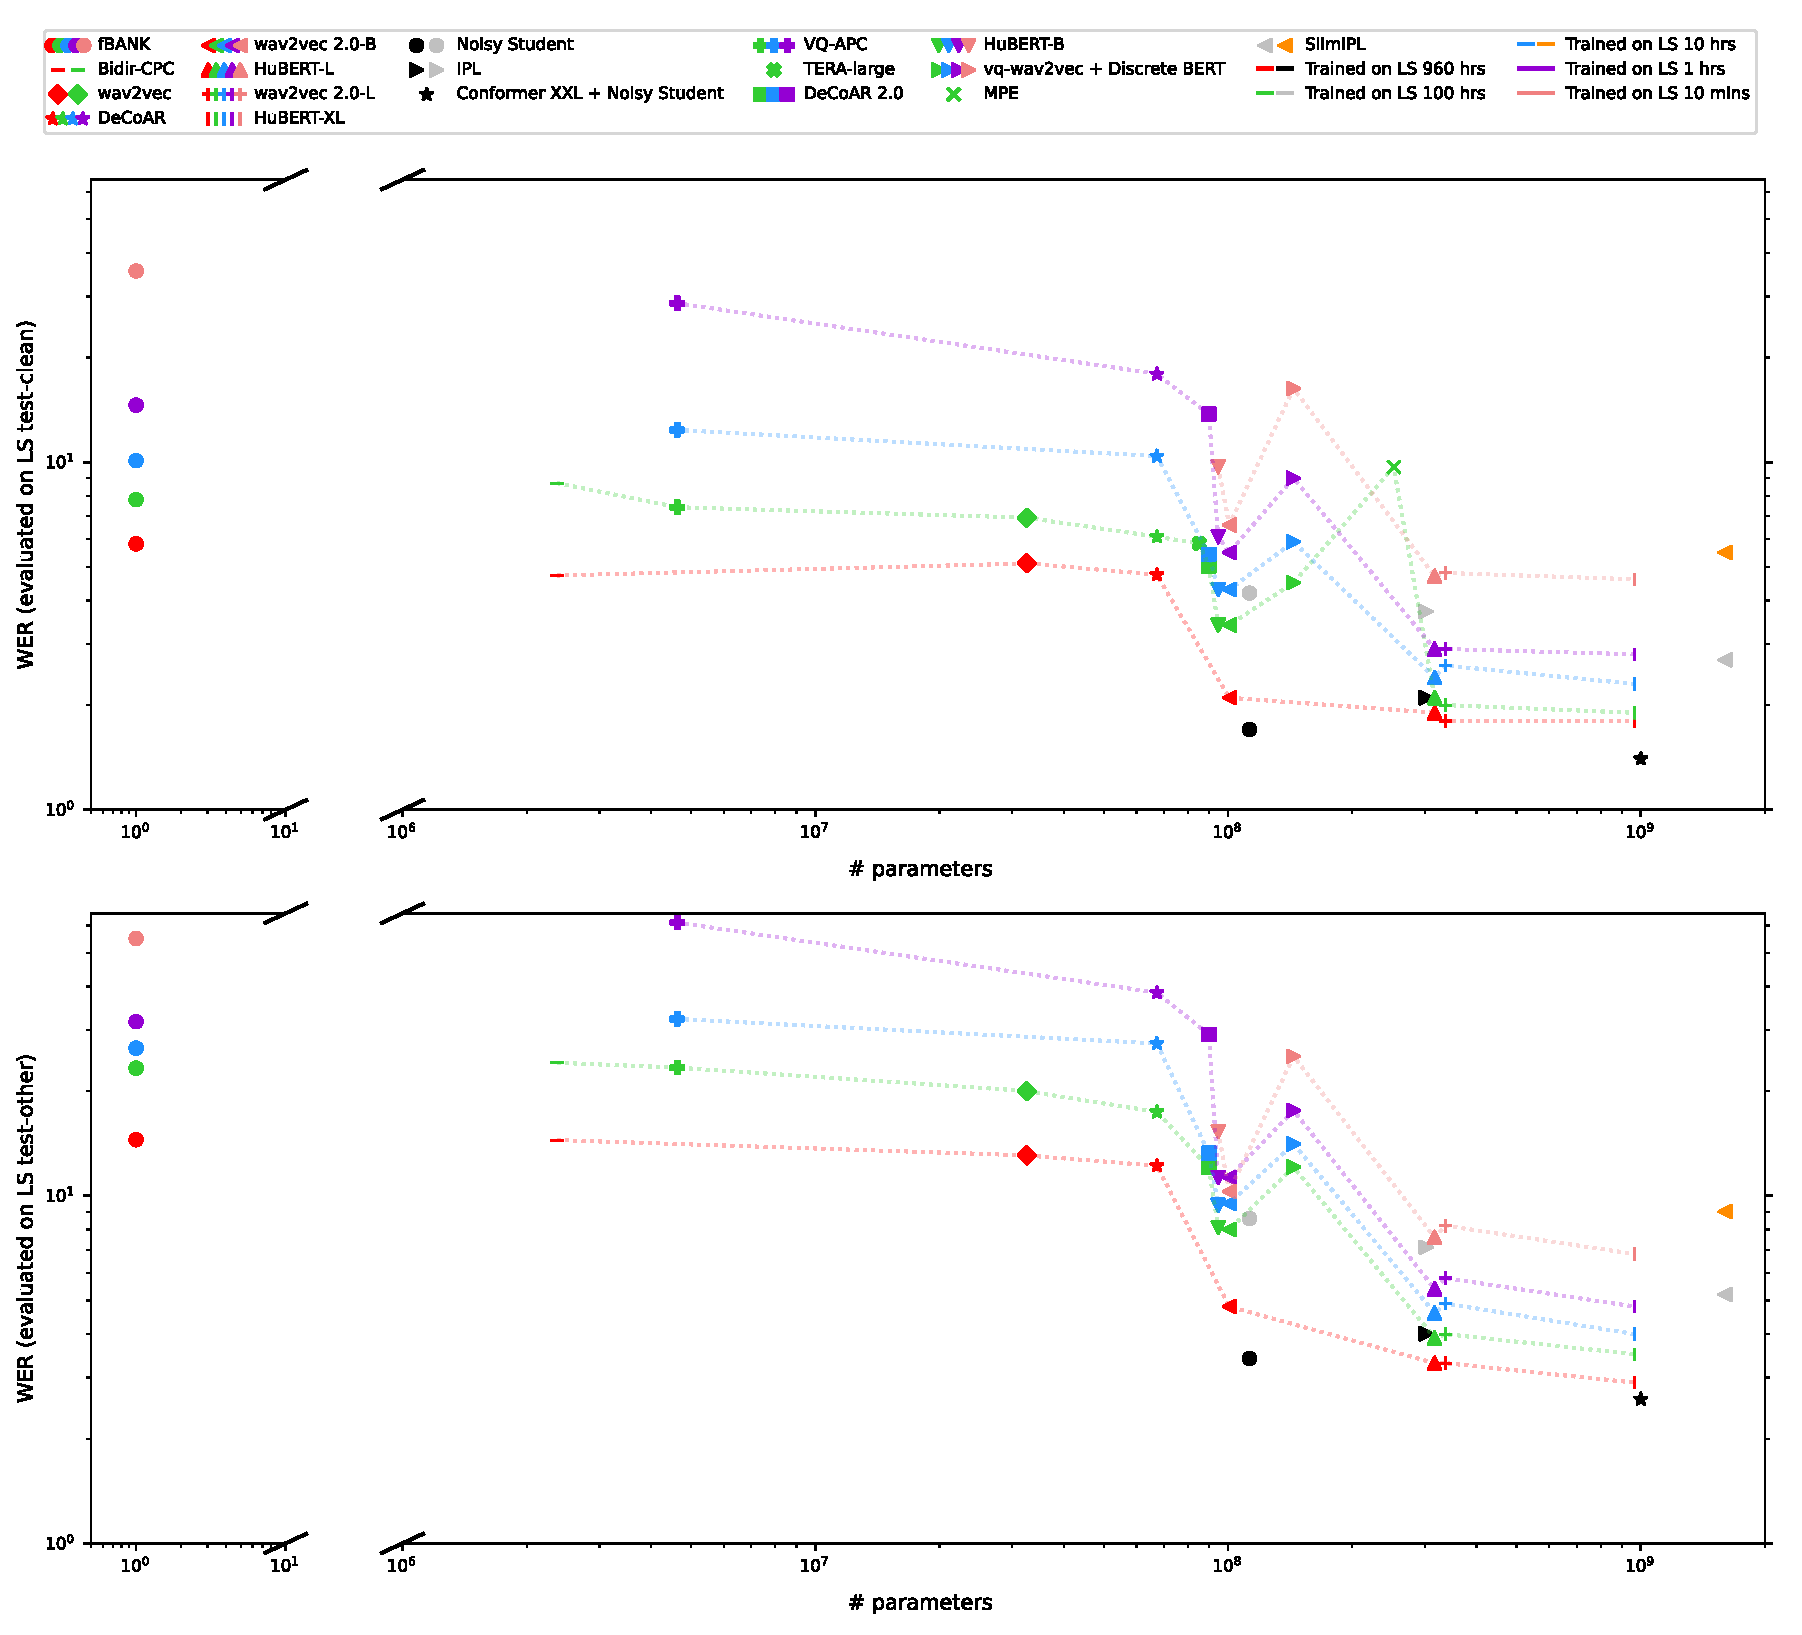
\includegraphics[width=1.0\textwidth]{paper_review/ls-test-clean-other.pdf}
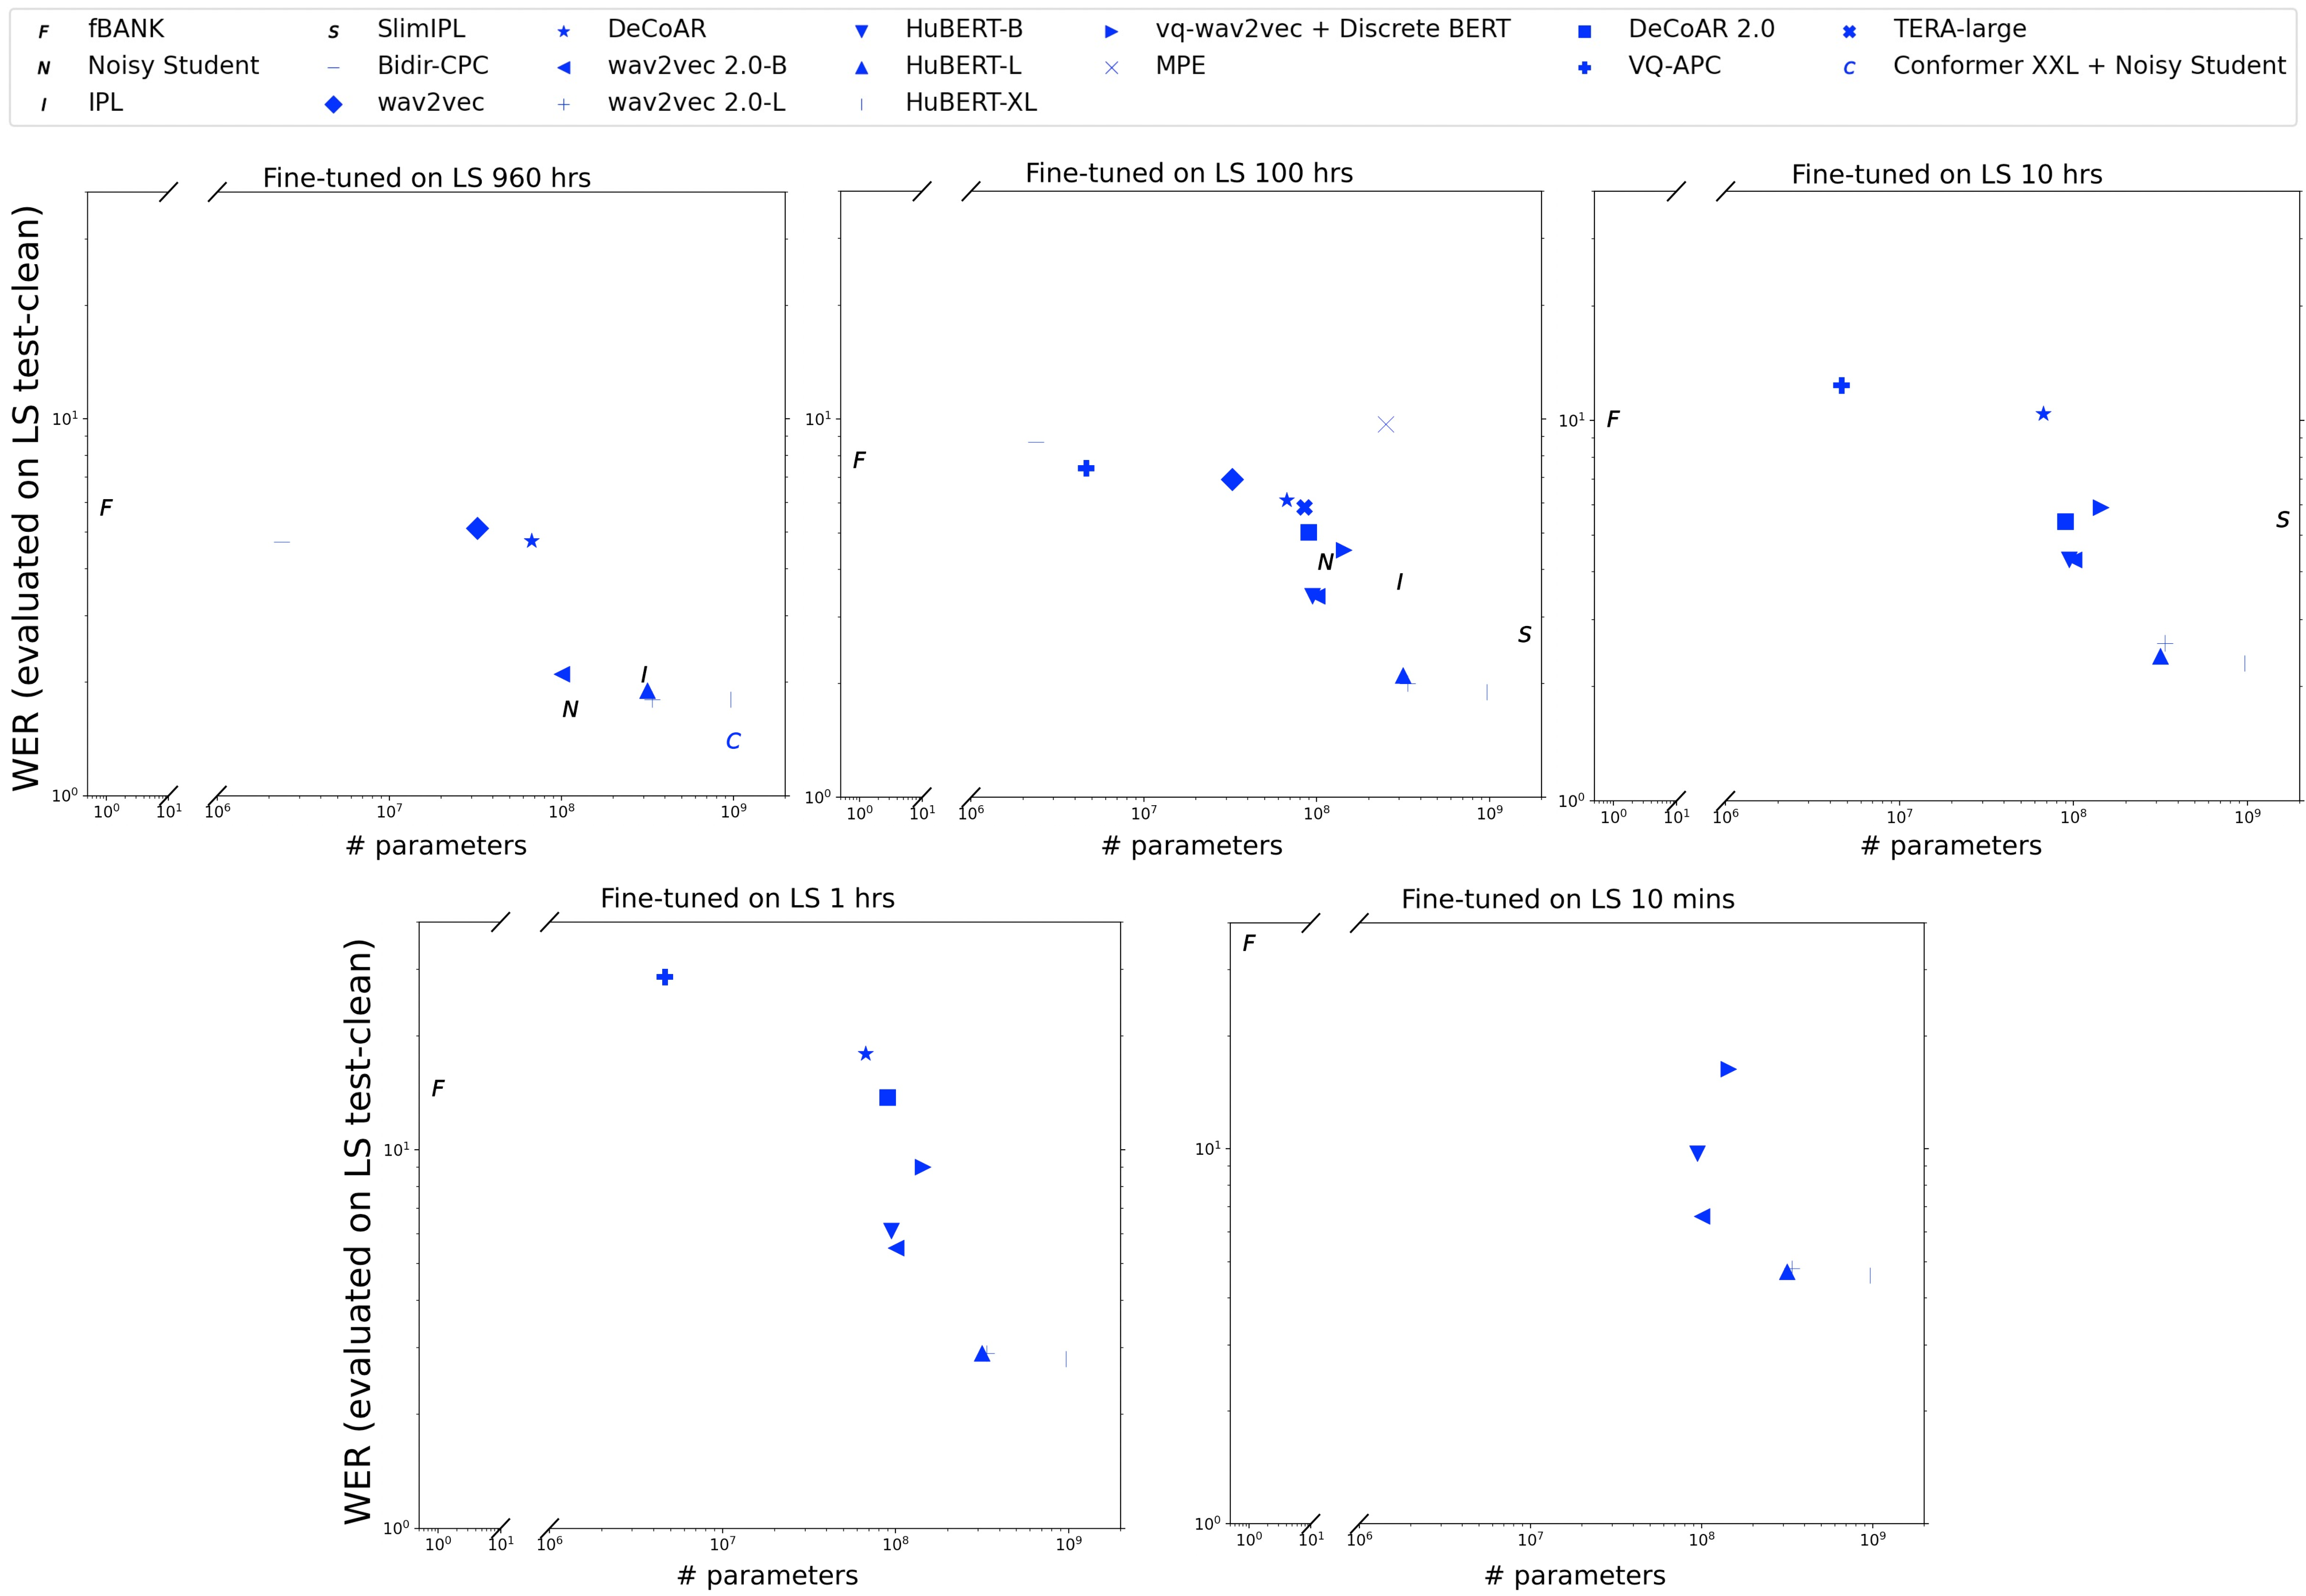
\includegraphics[width=0.9\textwidth]{paper_review/ls-test-clean-v2.pdf}
\caption{SSL performance on ASR WER (vertical axis) evaluated with
LS \textit{test-clean} split. Techniques are sorted based on the number of
model parameters along the horizontal axis. Markers in blue correspond to models initialized with various SSL
techniques and then fine-tuned using 960, 100, 10, 1 hour(s), and 10 minutes
respectively. The 960-hour training set is the aggregation of
\textit{train-clean-100}, \textit{train-clean-360}, and
\textit{train-other-500} splits. The 100-, 10-, 1-hour, and 10-minute sets
leverage \textit{train-clean-100} or its sampling, except for Bidir-CPC, which
samples 10\% of the training examples from the entire 960-hour corpus. For simplicity,
several SSL techniques are appended with suffixes \textit{B}, \textit{L},
\textit{XL}, or \textit{XXL} indicating the \textit{Base}, \textit{Large},
\textit{X-Large}, or \textit{XX-Large} variants specified in the original
publication. We also compare with baselines including the log mel filterbank (fBANK) and semi-supervised, self-training
approaches (iterative pseudo labeling (IPL)~\cite{xu2020iterative}, 
slimIPL~\cite{likhomanenko2020slimipl}, noisy student~\cite{park2020improved}). These approaches are visualized in black. Also, note that the current state of the art---conformer XXL + noisy student~\cite{zhang2020pushing}---is a combination of self-training and SSL techniques. Given the
diversity of the listed methods in experiment settings (e.g., pre-training corpora
and objectives, whether a language model is used in decoding, whether model
parameters are frozen in fine-tuning), readers should be careful that the superiority
of methods cannot be decided only based on lower WER numbers.}
\label{fig:asr_result_no_limit}
\end{figure*}


\subsection{Benchmark results and discussion} \label{sec:benchmark} 
Given the diversity of datasets and downstream tasks used to evaluate SSL
techniques in the literature, it is infeasible to discuss all 
experiment settings in this survey. Hence, due to their wide adoption for
experiments conducted by studies in both SSL and the speech community in
general, we focus first on ASR on the LS dataset to understand the
efficacy of SSL. We examine SSL techniques which report ASR results on the LS
\textit{test-clean} split, and summarize the published WER in
\cref{fig:asr_result_no_limit}. The ASR models were obtained first by using
unlabeled speech to pre-train a model with each SSL technique. The model was
then fine-tuned on labeled data by utilizing a supervised training objective.
Respectively, 960, 100, 10, 1 hour(s), and 10 minutes of labeled LS training data
were used for fine-tuning, as indicated in different panels of
\cref{fig:asr_result_no_limit} (see
the caption of \cref{fig:asr_result_no_limit} for more details).
Semi-supervised methods such as self-training, where a model is first trained
on labeled data to annotate unlabeled speech, and then subsequently trained on
combined golden and self-annotated label-speech pairs, are gaining popularity
in the speech community and have yielded competitive results. For comparison, we also
show performance from such methods (iterative pseudo labeling 
(IPL)~\cite{xu2020iterative}, slimIPL~\cite{likhomanenko2020slimipl}, noisy 
student~\cite{park2020improved}), as well as the current state of the art---conformer XXL + noisy
student~\cite{zhang2020pushing}---which augments SSL with various advanced
techniques including self-training. Furthermore, we illustrate in the figure
the performance of a baseline system \cite{yang21c_interspeech} based on log mel filterbank (fBANK), which is one of the most commonly used features designed by domain experts.
As observed in the figure, most SSL techniques outperform fBANK
features, and with the growing investment in model size, better performance is
achieved. The largest ones, such as wav2vec 2.0-L and HuBERT-L/XL, yield
% results competitive to the state of the art 
  competitive results                         % AMH: check
when the entire 960-hour of labeled data is used in
training/fine-tuning. The benefit of SSL, especially models with more parameters
like wav2vec 2.0 and HuBERT, becomes more evident when the labeling resources
become scarce. Compared to popular semi-supervised methods such as IPL,
slimIPL, and noisy student using 100 hours of labels, wav2vec~2.0 and HuBERT
achieve lower or competitive WERs with 1 hour or even 10 minutes of labeled
examples. The results are highly favorable for low-resource use cases, for instance when
expanding systems to new domains or languages for which large amounts of unlabeled
audio are available, since collecting labels for new conditions is often prohibitively
slow or costly.
% discuss the trend
%[Pick representative tasks and datasets and show the benefit of SSL, e.g., fewer fine-tuning/labeled data is required to achieve better/comparable performance] [talk about trend as well]  The plot suggests that ASR results have been increased significantly with the progress in SSL. Near SOTA performance can be achieved with much fewer training examples.  

In addition to the ASR task, where the current state of the art is achieved by a method
combining SSL pre-training and self-training 
techniques~\cite{zhang2020pushing}, SSL models 
% approach the state of the art 
  are competitive                % AMH: check
in other tasks, including IC,
SID, ASV, and QbE. We summarize the performance of these models and previous
non-SSL methods in \cref{table:sota_performance}. The results suggest that the
benefit of SSL is generalizable among tasks that require encoding 
information such as content, speaker, and semantics. As SSL research
gains more attention, we expect that SSL pre-trained models will 
achieve state-of-the-art results on an increasing number of tasks.

\begin{table}[ht]
  \centering
  \footnotesize
  \caption{Tasks where the state of the art is models with SSL pre-training.}
  \label{table:sota_performance}
  \renewcommand*\arraystretch{1.2}
  \begin{tabular}{llllll}  
    \toprule
    Tasks & Dataset & non-SSL & SSL \\
    \midrule
    ASR (WER $\downarrow$) & LS test-clean/other & 2.1/4.0 \cite{xu2020iterative} & 1.4/2.6 \cite{zhang2020pushing} \\ \hline
    IC (Acc $\uparrow$) & FSC & 98.8 \cite{lugosch19_interspeech} & 99.3\cite{chen2021unispeechsat} \\ \hline
    SID (Acc $\uparrow$) & VoxCeleb1 & 94.8 \cite{hajibabaei2018unified} & 95.5 \cite{chen2021wavlm} \\ \hline
    ASV (EER $\downarrow$) & VoxCeleb1 & 3.1 \cite{hajavi2021siamese} & 2.4 \cite{wang2021fine} \\ \hline
    QbE (MTWV $\uparrow$) & QUESST (EN) & 10.6 \cite{rodriguez2014gtts} & 11.2\cite{chen2021unispeechsat} \\

    %wav2vec-c
    %wav2vec-c \cite{sadhu21_interspeech} & Alexa-10k & ASR & \makecell[l]{Alexa-eval} & \makecell[l]{Alexa-eval} & \checkmark & 1k hrs \\ \hline
    %UniSpeech-SAT \cite{chen2021unispeechsat} & \makecell[l]{LL 60k hrs\\\;\;\;+ GigaSpeech-10k\\\;\;\;+ VP-24k} & Multi & SUPERB & SUPERB & \checkmark & Check SUPERB \cite{yang21c_interspeech} paper for details \\ \hline
    %WavLM \cite{chen2021wavlm} & \makecell[l]{LL 60k hrs\\\;\;\;+ GigaSpeech-10k\\\;\;\;+ VP-24k} & Multi & SUPERB & SUPERB & \checkmark & Check \cite{yang21c_interspeech} for details \\ \hline
    %\multirow{4}{*}[0mm]{XLS-R \cite{babu2021xlsr}} & \multirow{4}{*}[0mm]{\makecell[l]{VP-400k + MLS\\\;\;\;+ CV-dataset-7k + VL\\\;\;\;+ BBL}} & ASR & VP, MLS, CV-dataset, BBL, LS & VP, MLS, CV-dataset, BBL, LS & - & \multirow{4}{*}[0mm]{Check \cite{babu2021xlsr} for details} \\ \cline{3-6}
    %& & SID & VoxCeleb1 & VoxCeleb1 & \checkmark & \\ \cline{3-6}
    %& & ST & CoVoST-2 & CoVoST-2 & \checkmark & \\ \cline{3-6}
    %& & LID & VL & VL & - & \\ \hline

    \bottomrule
  \end{tabular}
\end{table}

Despite the obvious trend of increasing performance as more parameters and SSL
pre-training data are being used, numbers in \cref{fig:asr_result_no_limit} 
and \cref{table:sota_performance} are less comparable than might be expected.
The task performance is obtained from the original papers and is often
achieved with different downstream fine-tuning recipes, including various
language models (used in the ASR system), prediction heads (networks added to
SSL for downstream inference), or choices between fine-tuning the whole
networks or freezing the SSL encoders. For example, in the ASR task, HuBERT-L
and wav2vec~2.0-L leverage Transformer as their language model, while a 4-gram
language model trained on LS is used in DeCoAR~2.0. The lack of common and
established mechanisms to evaluate SSL techniques in downstream applications
makes it difficult to compare techniques fairly and understand their
capabilities. To address this challenge, there are increasing efforts to establish
benchmarks with shared downstream tasks, datasets, and downstream recipes. Such
efforts include SUPERB~\cite{yang21c_interspeech}, 
LeBenchmark~\cite{evain21_interspeech}, ZeroSpeech~\cite{dunbar2020zero},
HEAR \cite{pmlr-v176-turian22a},
NOSS~\cite{shor20_interspeech}, and HARES~\cite{wang2021towards}. 

SUPERB~\cite{yang21c_interspeech} is a benchmarking platform that allows the
SSL community to train, evaluate, and compare speech representations on
diverse downstream speech processing tasks, from acoustic and speaker identity
to paralinguistic and semantics. SUPERB consolidates downstream recipes to
focus on common and straightforward settings (e.g., prediction head
architectures, language models, hyperparameter spaces) to facilitate generalizable
and reproducible benchmarking of SSL techniques. SUPERB also encourages
researchers to innovate for efficient use of model parameters and computation
resources 
to democratize SSL beyond race among Big Tech.   % AMH: what does this mean?
LeBenchmark~\cite{evain21_interspeech} shares a vision similar to SUPERB and provides a
reproducible framework for assessing SSL in French with ASR, spoken language
understanding, speech translation, and emotion recognition. 
ZeroSpeech~\cite{dunbar2020zero} (described in more detail in \cref{zero_speech})
challenges the scientific community to build speech and language understanding
systems using zero expert resources 
%with the ultimate goal of bringing the systems to the services 
for millions of users of ``low-resource" languages.
%or in abnormal condition (dyslexia, autism, etc). ZeroSpeech offers evaluation for independent units in the system as well aggregation of multiple components. 
SSL techniques are also benchmarked with the ZeroSpeech 
challenge~\cite{tjandra20_interspeech, niekerk20b_interspeech}. Apart from the speech
community, researchers have also established HEAR (holistic evaluation of audio
representations) \cite{pmlr-v176-turian22a}, NOSS (non-semantic
speech benchmark)~\cite{shor20_interspeech}, and HARES (holistic audio
representation evaluation suite)~\cite{wang2021towards} to benchmark audio
representations. These efforts promote the creation of an audio embedding
that is as holistic as the human ear in interpreting speech, environmental
sound, and music. Given the significant need to understand and compare SSL techniques
fairly and comprehensively, we expect SSL benchmarking to remain an
active research area.

%SUPERB motivation: consolidating evaluation recipes to understand the capability of various SSL in a fair way. SUPERB designates the architectures of prediction heads for each downstream tasks [common architectures] [frozen] [generalizable, comparable, reproducible results]. [Results on tasks with such constraint conditions (mainly SUPERB but also from literatures imposing similar constraint).] [discussion on the results - competitive performance with simple downstream recipes] [More challenges, ZeroSpeech, HEAR ...]



%Librispeech 100h-960h \\
%Libri-light 10m, 1h, 10h - 60k \\
%SUPERB \\
%Add more
%Hear 2021 Challenge? (focus on audio, not only speech)




%!TEX root = ../thesis.tex

\section{Analysis of Self-Supervised Representations}
\label{analysis}

% {\color{blue} Katrin}\\
The previous sections have shown how self-supervised learning can result in
powerful representations that provide a robust starting point for several
downstream tasks. It is natural to ask if we can gain an even deeper
understanding of the nature of these representations, in order to further
optimize them or apply them to different problems.
What is the information encoded in these representations? How robust are they
to distributional shifts, and how dependent are they on the size of the
training data? Do they generalize across languages? What are the key
ingredients for training powerful representations: input data, network
architecture, training criterion, or all three? Can we predict their
performance on downstream tasks from their training behavior? This section
tries to answer these questions by summarizing several studies that analyze
self-supervised representations.

\subsection{Information content}

In \cite{pasad_layerwise_2021} wav2vec~2.0 representations were analyzed with
respect to their acoustic-linguistic information content at different
network layers. Three different mechanisms were used for this
purpose. The first of these is canonical correlation analysis (CCA),
which computes similarity scores between two continuous vectors
based on the maximum correlation of their linear projections.  These
can be used to judge the similarity of embeddings at different layers
with each other, with standard acoustic representations such as mel
filterbank features, or word embeddings derived from text. The second
method clusters continuous representation vectors and computes the
discrete mutual information between cluster IDs and phone or word
labels. The third method involves probing tasks: representation
vectors extracted from the network are used to perform simple
downstream tasks, in particular determining whether two acoustic segments
correspond to the same word, and a standard benchmark of 11 word
similarity tasks~\cite{faruqi14}. These are mostly used to gauge the
amount of lexical information present in the embeddings.  Using this
battery of tests the authors compared pre-trained models of varying
sizes as well as models fine-tuned for ASR. They found that pre-trained
models show an autoencoder-style behavior, with early layers showing
strong similarity with input features, intermediate layers diverging
more, and final layers reverting back to higher similarity with input
features and early layers. Generally, the earlier layers in wav2vec~2.0 
models encode acoustic information. The next set of layers encodes
phonetic class information, followed by word meaning information,
before reverting back to encoding phonetic/acoustic information. Thus,
extracting representations from the last layers for tasks that require
phonetic or word-related information may not be the best
strategy. Indeed, the authors of \cite{baevski2021unsupervised} show that a
phone classifier trained on each of the 24 frozen layers of a wav2vec~2.0 model
showed the lowest phone error rates
for layers 10--21 and higher error rates for the other layers. 
\cite{pasad_layerwise_2021} further show that fine-tuning the pre-trained model with a
character-level CTC training criterion changes the behavior of the
last layers (especially the final two layers), breaking the
autoencoder-style behavior and focusing the information encoded in the
last layers on orthographic-phonetic and word information. 

The peaking of class-relevant information in intermediate layers seems to be
common across different self-supervised learners and different modalities. In
an analysis of text-based Transformers trained with a masked language model
criterion~\cite{voita2019} observed a similar compression plus reconstruction
pattern. Interestingly, similar network behavior was also recently described
for self-supervised learners in computer vision: using a contrastive
self-supervised learner (SimCLR) that optimizes for augmentation invariance,
\cite{grigg2021self} show that it is the intermediate representations that most
closely approximate information learned in a supervised way, i.e., they
provide more class information than the representations from final layers. This
is similar to the findings described above for wav2vec~2.0 without fine-tuning,
where intermediate layers provide more information about phone and word
classes.

Self-supervised representations may encode other information besides phonetic
classes or words, for example, channel, language, speaker, and sentiment
information. 
\edit{It is shown that the per-utterance mean of CPC features captures speaker information to a large extent\cite{van2021analyzing}.}
Location of information pertaining to speakers vs.\ language classes was
analyzed in \cite{ling20odyssey} for a 12-layer BERTphone model. This model
combines a self-supervised masked reconstruction loss with a phone-based CTC
loss to produce representations	for speaker recognition and language
identification. By	analyzing the weights	of a linear combination	of layer
representations for these two downstream tasks, it was	shown that language
recognition draws on representation	from higher layers (peaking at layer~10)
whereas speaker recognition benefited from layers at positions 6, 9, and 12.
This may indicate that language recognition relies more on higher-level
phonetic information whereas speaker recognition uses a combination of
acoustic and phonetic information. In a recent study~\cite{chen_wavlm_2021} the
same technique was used to identify layer contributions for the downstream
SUPERB benchmark tasks in the WavLM model. For a smaller model (95M parameters)
it was again confirmed that lower layers encode speaker-related information
necessary for speaker diarization and verification whereas higher layers encode
phonetic and semantic information. Another study~\cite{wang2021layersup} used
explicit self-supervised loss at the intermediate layers rather than just the
output layer of a HuBERT model in order to enforce better learning of phonetic
information. The resulting model was indeed better at downstream tasks
requiring information about phonetic content, such as phone recognition, ASR,
and keyword spotting, but worse at speaker-related tasks like speaker
diarization and verification. 

%Hung-yi Lee: My group also has a paper analyzing the attention of self-supervised speech model (https://arxiv.org/abs/2006.03265). I will include some findings in this subsection later.
Most self-supervised learning approaches rely on a Transformer architecture for
the representation model. In \cite{AnalyzeAttention} the attention patterns in
generatively trained Transformer representation models were analyzed.
Self-attention heads were grouped into three categories: diagonal, vertical,
and global. It was found that the diagonal head focuses on neighbors and is
highly correlated with phoneme boundaries, whereas the vertical head focuses on
specific phonemes in the utterance. Global heads were found to be redundant as
removing them resulted in faster inference time and higher performance.

\subsection{Training criterion}
In \cite{chung2021}, representations based on different training criteria
(masked predictive coding, contrastive predictive coding, and autoregressive
predictive coding) were compared  and analyzed with respect to the correlation
between their training loss and performance on both phone discrimination and
speaker classification probing tasks. It was observed that the autoregressive
predictive coding loss showed the strongest correlation with downstream
performance on both tasks; however, models were not further analyzed
internally. An evaluation of the similarity of representations trained
according to the three criteria above (but with different architectures and
directionality of contextual information) also showed that it is the training
criterion that most influences the information encoded in the representations,
not the architecture of the learner or the directionality of the input. 

A similar insight was obtained in \cite{zhou2020}, which compared vq-vae and
vq-wav2vec with respect to their ability to discover phonetic units.
The vq-vae model extracts continuous features from the audio signal; a
quantizer then  maps them into a discrete space, and a decoder is trained to
reconstruct the original audio conditioned on the latent discrete
representation and the past acoustic observations. By contrast, vq-wav2vec
predicts future latent discrete representations based on contextualized
embeddings of past discrete representations, in a CPC-style way. The models
were evaluated according to their ability to discover phonetic units (as
measured by phone recognition error rate on TIMIT, and the ZeroSpeech ABX task
(see \cref{sec:zero} for more details)), and it was found that the predictive vq-wav2vec
model fared better than the autoencoder-like vq-vae model, most likely due to
its superior ability to model temporal dynamics.

\subsection{Effects of data and model size}
\label{subsec:modelsize}

How does the performance of self-supervised models change in relation to the
amount of training data, and in relation to the size (number of parameters) of
the model?
Several studies have demonstrated better downstream performance when using
larger datasets~\cite{rivi20, kawakami2020learning, chen_wavlm_2021}. For
example,
\cite{kawakami2020learning} compared representations learned by a bidirectional
CPC model from the standard 960 hour LS corpus and a corpus of 8,000 hours of
diverse speech from multiple sources.\textsuperscript{\ref{footnote:CPC-8k}}
Not surprisingly, an ASR model trained on top of these representations
performed better when representations were learned from the larger dataset. 
Although the precise relationship between data size and performance has not
been quantified, we can assume that it follows a law of diminishing returns (or
power law), 
similar to observations for most data-intensive machine learning tasks.
In addition to the size of the dataset, the diversity of the data also seems
to play a role, although this was not quantified in this study. However, recent
experiments with larger and more diverse data collections~\cite{chen_wavlm_2021}
confirm this assumption, as do 
explicit investigations of domain shift robustness (see
\cref{subsec:robustness} below). 

\edit{The relation between model sizes and downstream performances have also been investigated \cite{pue2021scaling,versteegh2015zero}.}
Using the Mockingjay 
model~\cite{liu_mockingjay_2020}, the authors in \cite{pue2021scaling} attempt to establish a relationship between
model size and self-supervised \ensuremath{L_1} loss and demonstrate that it approximately
follows a power law. Model size and accuracy on downstream phone
classification and speaker recognition tasks are positively correlated but do not
exactly follow a power law; rather, the accuracy saturates as models increase in
size, possibly due to the lack of a corresponding expansion in training data
size.

\subsection{Robustness and transferability}
\label{subsec:robustness}

It is well known that traditional speech features like MFCCs lack
robustness against environmental effects such as additive noise,
reverberation, accents, etc., that cause differences in the distributions of
speech features.
Do pre-trained representations offer greater robustness against distributional
shifts? 
One study~\cite{kawakami2020learning} compared pre-trained
representations from a CPC model against MFCCs and 
found pre-trained representations to be more robust to mismatches between
training and test data. The 
training data consisted of clean, read speech (LS)
whereas test data consisted of the Switchboard corpus and TED talks. The
distributional shifts here may stem from both the acoustics (microphone, room
reverberation) as well as
lexical effects related to topic and style, as well as differences in speaker
characteristics such as accent. 
Similar problems were also investigated using HuBERT and wav2vec~2.0 models in
\cite{chang2021exploration}.
In \cite{robustw2v2} domain effects were studied in greater detail using 
datasets from six different domains. In particular, the authors focused on the
usefulness of adding out-of-domain data to pre-training. The general
conclusions are that pre-training on more and diverse domains is preferable:
models pre-trained on more domains performed better than those pre-trained on
fewer when tested on held-out domains, regardless of which additional
labeled data was used for fine-tuning. Adding in-domain unlabeled data---if
available---to pre-training improves performance robustly; however, even
out-of-domain unlabeled data is helpful and closes  66--73\% of the performance
gap between the ideal setting of in-domain labeled data and a competitive
supervised out-of-domain model. 
 
In \cite{rivi20} the effectiveness of CPC-trained representations for
phone discrimination tasks was compared across several languages. It
was found that representations pre-trained only on English successfully
enabled phone discrimination in 10 other languages, rivaling
supervised methods in accuracy in low-data regimes (1h of labeled data
per language). Thus, self-supervised pre-training enables the model to
learn contextualized speech features that generalize across different
languages. In \cite{conneau20xling}, a wav2vec~2.0 model was trained on data
from multiple different languages and different corpora (Babel, Common Voice,
and multilingual LS)
jointly, followed by fine-tuning for each individual language. The largest
model covers 53 languages in total
and consists of 56,000 hours of speech. Compared to monolingual pre-training,
even smaller models trained on only ten languages improve performance
substantially on a downstream character-based ASR task. Low-resource languages
with little labeled data improve the most under this training regime.
Multilingual representations also resulted in competitive performance (lower
character error rate than monolingual representations) for languages not
present in the training dataset, again showing that unsupervised pre-trained
representations can learn generic features of the speech signal that generalize
across different languages. The study also found that sharing data from closely
related languages is more beneficial than combining distant languages. An
analysis of language clusters in the shared discrete latent representation
space revealed that similar languages do indeed show a higher degree of sharing
of discrete tokens. 
Finally, one might ask whether the interpretation of representations extracted
from different layers of a self-supervised models also generalizes to the
multilingual setting. Experiments in \cite{baevski2021unsupervised} on phone
recognition in eight languages based on the different layers of the
multilingual wav2vec~2.0 XLSR-53 model indicate that this is indeed the case:
phone error rates showed the same pattern as in the monolingual (English)
scenario, with lower phone error rates for middle layers as opposed to
earlier/later layers. 





 
%!TEX root = ../thesis.tex

\section{From representation learning to zero resources}
\label{sec:zero}

% {\color{black} Reviewer: TNS, Abdo, Hung-yi Lee }\\
% \kl{We discussed in our last meeting that I would add a pointer in this section to the acoustic word embedding section.  However, I'm not quite sure what the right spot for it is, so waiting for this section to stabilize a bit more first.}


In the SSL framework, speech representations can be
learned and used in various downstream tasks to achieve competitive, robust,
and transferable performance, as shown in
\crefrange{section:benchmark}{analysis}. 
However, labeled data is still required. 
For example, in ASR, utterances and their manual transcriptions are needed to learn downstream models or fine-tune representation models. 
Can a model learn without any labeled data? 
In \cref{secsec:unpaired}, we show how to learn ASR models without any paired audio and text and how SSL improves the framework.
In addition, many languages have no writing system. 
In \cref{subsec:zero}, the SSL representation is further used in scenarios where text data is unavailable.

\subsection{Unpaired text and audio} \label{secsec:unpaired}
% What are we going to do % how to match
%In the self-supervised learning framework, speech representations can be learned and used in the downstream tasks, but some labeled data for finetuning is needed.

\begin{sidewaystable}
\centering
\caption[Performance of models within unsupervised ASR.]{
	Unsupervised ASR.
	TIMIT numbers are phoneme error rates (PER), while the numbers for
	LibriSpeech are word error rates (WER).
	SWC $=$ spoken word classifier, ST $=$ speech translation.
	All speech and text are in English if not specified. 
	\textcolor{black}{The references in the table are sorted according to the date of publication.}}
	\label{fig:unsupervisedASR}
	\resizebox*{\textwidth}{!}{%
	{\renewcommand*\arraystretch{1.4}}
	\begin{tabular}{cllllll}
	\toprule
	Reference & Speech representation & Speech segmentation  & Token & Mapping approach & Refinement  & Results  \\ 
	\midrule
	\parencite{liu_completely_2018}& Audio word2vec~\parencite{wang_segmental_2018} & Oracle & Phoneme & \edit{Adversarial Training~\parencite{gulrajani_improved_2017}} & - & TIMIT (PER): 63.6\%  \\ %Submitted on 1 Apr 2018
	\midrule
	\parencite{chung_unsupervised_2018} & Speech2vec~\parencite{chung_speech2vec_2018} & BES-GMM~\parencite{kamper_segmental_2017} &  Word2Vec & \edit{Adversarial Training~\parencite{conneau_word_2018}} & Self-training & SWC (Acc): 10.9\%  \\ %Submitted on 18 May 2018
	%https://arxiv.org/pdf/1805.07467.pdf %The text embeddings were obtained by training Word2Vec on the transcriptions using the fastText implementation without subword information [3].
	\midrule
	
	\parencite{chung_unsupervised_2019a} & \tabincell{l}{Speech2vec\\(English)} & Oracle & \tabincell{c}{Word2Vec\\(French)} & VecMap~\parencite{artetxe_robust_2018} & \tabincell{l}{LM rescore,\\sequence DAE} & ST (BLEU): 10.8\%   \\ %[Submitted on 4 Nov 2018]
	\midrule
	
	\parencite{yeh_unsupervised_2019} & MFCC & GAS~\parencite{wang_gate_2017} & Phoneme & Empirical-ODM~\parencite{liu_unsupervised_2017} & Self-training &  TIMIT (PER):  41.6\%  \\ %Submitted on 23 Dec 2018
	\midrule

	\parencite{chen_completely_2019} & MFCC & GAS  & Phoneme & \edit{Adversarial Training~\parencite{gulrajani_improved_2017}} & Self-training &  TIMIT (PER):  33.1\%   \\
	\midrule

	\parencite{baevski_unsupervised_2021} & Wav2vec 2.0~\parencite{baevski_wav2vec_2020} & $k$-means & Phoneme &\edit{Adversarial Training~\parencite{gulrajani_improved_2017}} & Self-training & \tabincell{l}{TIMIT (PER):  18.6\%, \\ LibriSpeech (WER): 5.9\%}   \\
	\midrule
	
	\textcolor{black}{\parencite{klejch_deciphering_2022}} & \textcolor{black}{\tabincell{l}{Universal Phone \\ Recogniser}} & - & \textcolor{black}{Grapheme} & \textcolor{black}{Decipherment~\parencite{ravi_deciphering_2011}} & \textcolor{black}{Self-training} & \textcolor{black}{\tabincell{l}{GlobalPhone: 32.5\% to just 1.9\% \\ worse than supervised models} }  \\ %ubmitted on 12 Nov 2021 %m 32.5% to just 1.9% absolute worse than the equivalent fully supervised models trained on the same data
	\midrule
	\textcolor{black}{\parencite{liu_endtoend_2023}} & \textcolor{black}{Wav2vec 2.0~\parencite{baevski_wav2vec_2020} }& - & \textcolor{black}{Phoneme} & \textcolor{black}{Adversarial Training~\parencite{gulrajani_improved_2017}} & \textcolor{black}{Self-training} & \textcolor{black}{LibriSpeech (WER): 6.3\%}   \\
	\midrule

	\textcolor{black}{\parencite{liu_endtoend_2023}} & \textcolor{black}{Wav2vec 2.0~\parencite{baevski_wav2vec_2020}} & - & \textcolor{black}{Grapheme} & \textcolor{black}{Adversarial Training~\parencite{gulrajani_improved_2017}} & \textcolor{black}{Self-training} & \textcolor{black}{LJSpeech (WER): 64.0\%}  \\


	%e MUSE [7] and VecMap [8], n
	%The numbers in the section of unsupervised methods denoted as BLEU score (%) of VecMap /
	%BLEU score (%) of MUSE 10.8 / 6.2
	%11.3 / 7.3
	%https://arxiv.org/pdf/1811.01307.pdf
	\bottomrule
	\end{tabular}}
\end{sidewaystable}



\paragraph{Unsupervised ASR}
% {\color{black} Hung-yi}\\

If only unpaired speech and text are available, that is, the text is not a
manual transcription of speech, can the machine learn how to transcribe speech
into text?
This scenario is called \textit{unsupervised ASR}, and the framework is as
below. 
Given a set of unlabeled utterances $\mathcal{S}=\{S_1, S_2, ..., S_N\}$  and a
set of sentences $\mathcal{Y}=\{Y_1, Y_2, ..., Y_M\}$,\footnote{Note that
the speech and text are not paired, that is, $Y_i$ is not the transcription of
$S_i$.} a mapping function~$F$, which can take an utterance~$S$ as input and
generate its transcription, is learned from data. 
\Cref{fig:unsupervisedASR} summarizes recent work on unsupervised ASR,
including the speech representation used, the algorithm used to learn the
mapping without supervision, and the results. Below, we will discuss these
methods in more detail.


Adversarial training~\parencite{goodfellow_generative_2014,arjovsky_wasserstein_2017, gulrajani_improved_2017} is one common way to learn such a 
mapping function. 
The framework includes a discriminator and a generator.
The mapping function~$F$ plays the role of the generator, which takes speech utterances as input and outputs text.
The discriminator learns to distinguish real text from the generated
output; the generator learns to ``fool'' the discriminator.
The generator and the discriminator are trained in an iterative, 
interleaved way. 
After the training, the generator serves as the speech recognition model.
\edit{
There is a large amount of work using gradient penalty in the objective of training discriminators~\parencite{liu_completely_2018,chen_completely_2019,baevski_unsupervised_2021,liu_endtoend_2023}, which is inspired by Improved Wasserstein Generative Adversarial Network (WGAN)~\parencite{gulrajani_improved_2017}.
}
\textcolor{black}{
Other ways to map speech and text include via segmental empirical output distribution matching (segmental empirical-ODM)~\parencite{yeh_unsupervised_2019} and decipherment algorithm~\parencite{klejch_deciphering_2022}.}

% Difficulty of unsupervised ASR (v.s. unsupervised MT)
Success in unsupervised neural machine translation
(MT)~\parencite{artetxe_unsupervised_2018, conneau_word_2018, lample_unsupervised_2018}
has inspired innovative exploration of various unsupervised ASR algorithms.
If learning a translation model from unaligned sentences in two languages is
possible, considering speech and text as two different languages, learning the
mapping relationship from speech space to text space without an alignment 
% is not impossible.
  should likewise be possible.   % AMH: check
However, there are differences between unsupervised MT and unsupervised
ASR.
In unsupervised MT, most discrete source tokens can be mapped to specific
target tokens representing the same meaning. 
However, because speech has segmental structures, in unsupervised ASR, each text
token maps to a segment of consecutive acoustic features of variable length in
an utterance.
The generator is supposed to learn the segmental structure of an utterance
because information like token boundaries is not directly available.
This makes unsupervised ASR more challenging than unsupervised MT.

% how to represent audio
For unsupervised ASR to be feasible, the common idea is to make the speech and text units close to each other.
For the text side, word sequences can be transformed into phoneme sequences if a lexicon is available. 
On the other hand, we must first convert the speech signal into something close to phonemes. 
To achieve that, most studies on unsupervised ASR use a phoneme
segmentation module before the generator to segment utterances into
phoneme-level
segments~\parencite{liu_completely_2018,chen_completely_2019,yeh_unsupervised_2019}. 
A representation vector or a token then represents each phoneme-level segment. 
It is easier for the generator to map each segment-level representation 
or token to the correct phoneme when the representation or token is highly correlated to the phonemes.
Wav2vec-U~\parencite{baevski_unsupervised_2021} selects the input feature from different layers of wave2vec~2.0~\parencite{baevski_wav2vec_2020}.
The selection criterion is based on analysis of the phonetic information in each layer.
\textcolor{black}{
If a universal phone recognizer trained from a diverse set of languages is available, it is another way to transcribe speech into phone-level tokens~\parencite{klejch_deciphering_2022}.}
Another series of work is to transform a word into a word embedding. 
\parencite{chung_unsupervised_2018,chung_unsupervised_2019a} use adversarial training to map the word-level
speech embedding space~\parencite{chung_speech2vec_2018} to the word embedding space
and achieve promising performance on spoken word classification, speech
translation, and spoken word retrieval.
\Cref{fig:unsupervisedASR} summarizes the various ways to segment speech and represent speech and text in each reference.  

%Hung-yi Lee: I comment this paragraph first.
\begin{comment}
%Hung-yi Lee: This paragraph is not finished yet.
\TNS{if we are limited on space,we can consider removing some of the detail of the various algorithms}
\TNS{split into 2 sentences, also have a connection to the previous para}
\parencite{liu_completely_2018} is the first work to successfully achieve unsupervised
phoneme recognition by first clustering phoneme-level
embeddings~\parencite{chung_audio_2016,wang_segmental_2018} into a set of
tokens and then using GAN to learn the mapping relationship between tokens and
phonemes. 
However, in \parencite{liu_completely_2018}, oracle phoneme segmentation is still
required to get reasonable performance. 
\parencite{chen_completely_2019,yeh_unsupervised_2019} uses gate activation signals
(GAS)~\parencite{wang_gate_2017} to get the phoneme-level segmentation, which is
unsupervised. 
%However, the loss term in~\parencite{yeh_unsupervised_2019} includes an empirical average over all segments inside a logarithmic function, which can be biased if we sample this empirical average by a mini-batch average. \parencite{liu2017unsupervised} therefore use an extremely large batch size during training to reduce the biasing problem.
%These problems are handled by another work~\parencite{chen_completely_2019}.
%\parencite{chen_completely_2019} removes the quantization step.
%Compared to~\parencite{yeh_unsupervised_2019}, the discriminator in~\parencite{chen_completely_2019} considers all possible information from the text dataset, not limited to the n-gram local statistics.
%Besides, \parencite{chen_completely_2019} works well with a reasonable batch size, which makes it feasible when the computational resource is limited.
Wav2vec-U~\parencite{baevski_unsupervised_2021} selects the input feature from
different layers of wave2vec 2.0~\parencite{baevski_wav2vec_2020}, a self-supervised
model.
The selecting criterion is the PER by training a linear model in a supervised manner. 
%Should we mention this?
Wav2vec-U uses $k$-means to cluster the selected features, and the boundaries
are drawn whenever the clustered index changes.
%Wave2vec-U tends to generate more segments compared to the oracle phoneme-level segments. For example, their segmentation gives 0.93 precision, the ratio of the oracle phoneme-level boundaries being hit, and 0.38 recall, the ratio of the generated boundaries hit the oracle phoneme-level boundaries.
While Wav2vec-U merges the neighboring segments containing the same predicted
labels in each step of GAN training, this design can be viewed as refining the
segmentation implicitly.  
%Should we mention this?
%At generator output, the wav2vec-U will combine the neighboring predicted posterior containing the same predicted label into a predicted posterior.
\end{comment}

%In \parencite{chung_unsupervised_2018, chung_unsupervised_2019a}, the word boundaries are also generated automatically with speech only. 
%However, \parencite{chung_unsupervised_2018, chung_unsupervised_2019a} need oracle boundaries, therefore not completely unsupervised as the framework proposed in this paper.

% more improvement: iterative training, development 
As shown in \cref{fig:unsupervisedASR}, most studies use
\textit{self-training} to refine the models.
% to achieve better performance.  % AMH: redundant
In self-training, the generator serves as the first-version phoneme recognition model.
Inputting unpaired speech to the generator generates the corresponding
``pseudo transcription''. 
We then view the speech utterances and their pseudo transcriptions as paired
data which we use to train a model in a supervised manner.
Although the pseudo transcriptions have more errors than oracle
transcriptions, experiments show that training models on pseudo
transcriptions still significantly boosts performance compared to the
first-version model.
%With the new model, we can further obtain new transcriptions.
%The iteration will continue until the performance converges. 

%Using performance to end this section.
Wav2vec-U~\parencite{baevski_unsupervised_2021} achieved state-of-the-art results at the time, which suggests that representation learning is
essential for the success of unsupervised ASR.
It achieved an 11.3\% phoneme error rate on the TIMIT benchmark. 
On the LS benchmark, wav2vec-U achieved a 5.9\% \edit{WER} on
\emph{test-other}, rivaling some of the best published systems trained on 960 hours of labeled data from only two years earlier. 
\textcolor{black}{
And wav2vec-U 2.0~\parencite{liu_endtoend_2023} further removes the requirement of the segmentation stage, so the unsupervised ASR model can be learned in an end-to-end style.}
The robustness of wav2vec-U was further analyzed with respect to 
domain-mismatch scenarios in which the domains of unpaired
speech and text were different~\parencite{lin_analyzing_2022}.
Experimental results showed that domain mismatch leads to inferior performance, but a representation model pre-trained on the targeted speech domain extracts better representations and reduces this drop in performance.

%Hung-yi: The technique below is very important. But I think it is fine to ignore this part in a reviewe paper due to space limitation. 
\begin{comment}
In unsupervised learning, how to determine the hyperparameters is an issue. 
In a typical supervised framework, hyperparameter tuning is done by a
development set, which includes labeled data.
In an unsupervised setting, the existence of this kind of development is tricky. %Is tricky a correct term?
The existence of such kind of development set means the presence of the labeled
data.
Therefore, wav2vec-U~\parencite{baevski_unsupervised_2021} develops a new approach to
determine the hyperparameters without a labeled development set. 
%should I provide more details? 
\end{comment}

%Hung-yi: A series of work (most from MS) focuses on meager resources but not wholly unsupervised. Perhaps we have to mention the papers.


\paragraph{ASR-TTS}
%{\color{black} Shinji}\\
%{\color{black} Hung-yi: In the last meeting, we discussed the connection between this section and self-supervised learning. In addition to looking for papers using self-supervision to improve the ASR-TTS framework here, I think there may be another direction. Can we regard this ASR-TTS framework as a kind of self-supervised learning? ASR-TTS is similar to an autoencoder, and the output of ASR is "latent representation". In other words, this section describes a special self-supervised learning method, whose representation is expressed as "text."}\\
%{\color{black} Hung-yi: However, the above idea sounds tricky. In addition, the ``ASR-TTS'' autoencoder is learned by semi-supervised, not self-supervised.}
% AMH: to make the paper more consistent, I recommend changing all $f^{\mathrm{asr}}$ to $f_{\mathrm{asr}}$
Here we describe an alternative approach by which to train an ASR and \edit{text-to-speech (TTS)} system
based on unpaired text and audio. The ASR-TTS framework, which \edit{combines the ASR} and
TTS systems in a cascaded manner,
can be regarded as an autoencoder, where the encoder~$f$
corresponds to the ASR module and the decoder~$g$ corresponds to the TTS module.
In this framework, we consider the intermediate ASR output as a latent
representation; the framework as a whole can be regarded as a variant of
self-supervised learning.\footnote{However, to make this complicated
system work, we often require that data is paired. Therefore, in practice,
ASR-TTS and other methods described in this section are categorized as
semi-supervised learning.}

The ASR-TTS framework can jointly optimize both ASR and TTS \edit{without using paired data}~\parencite{tjandra_listening_2017,hori_cycleconsistency_2019,wang_improving_2020}.
A speech chain~\parencite{tjandra_listening_2017,tjandra_machine_2018} is one 
successful way to utilize audio-only and text-only data to train both
end-to-end ASR/TTS models.
This approach first prepares pre-trained ASR model \edit{
$f_{\mathrm{asr}}(X)$ with acoustic input $X$ and pre-trained TTS model $g_{\mathrm{tts}}(Y)$ with text input $Y$.
By following the TTS system with an ASR system, we generate new 
acoustic feature sequence~$\hat{X}$, which must be close to the original input~$X$.
Thus, we design a loss function $\mathcal{L}_{\mathrm{asr} \rightarrow \mathrm{tts}}(X, \hat{X})$, where $\hat{X}$ is generated by
%and~$\hat{X}$:
%\begin{equation}
%    \mathcal{L}_{\mathrm{asr} \rightarrow \mathrm{tts}} (X, \hat{X}),
%\end{equation}    
%where
\begin{equation}
    \hat{X} = g_{\mathrm{tts}}(f_{\mathrm{asr}}(X)) \enspace .
    \label{eq:asr-tts}
\end{equation}
Thus, we train the ASR model (or both ASR and TTS models) using only
the acoustic input by minimizing $\mathcal{L}_{\mathrm{asr} \rightarrow \mathrm{tts}}$.  
%\begin{equation}
%\hat{\theta}_{\mathrm{asr}} = \arg \min _{\theta_{\mathrm{asr}}} \mathcal{L}(Y, \hat{Y}; \theta_{\mathrm{asr}}, \theta_{\mathrm{tts}}).
%\end{equation}
Note that this approach does not require the supervised text data~$Y$}.
As an analogy to the generative approach in \cref{sec:generative}, the
intermediate ASR output~$\hat{Y}$ can be regarded as the latent representation~$Z$.

The other cycle with the text-only data~$Y$ is also accomplished by the
concatenated TTS-ASR systems:\edit{
\begin{equation}
    \hat{Y} = f_{\mathrm{asr}}(g_{\mathrm{tts}}(Y)) \enspace .
    \label{eq:tts-asr}
\end{equation}
Similarly, this approach does not require the supervised audio data~$X$, and the
intermediate TTS output~$\hat{X}$ can be regarded as the latent representation~$Z$}.
Although this approach initially freezes either the ASR or TTS model, 
extensions of this study~\parencite{hori_cycleconsistency_2019,tjandra_endtoend_2019,baskar_semisupervised_2019}
implement the joint training of both ASR and TTS parameters using 
REINFORCE~\parencite{williams_simple_1992} and straight-through estimators.

An emerging technique uses a well-trained TTS system to generate
speech and text data from text-only data.
This technique is a sub-problem of the TTS-ASR approach formulated in
\eqref{eq:tts-asr} in which we fix the TTS system part and estimate only the ASR
parameters. 
For example, a huge amount of text resources can be obtained from the web
and document archives without corresponding audio data.
%Self-supervised learning in this paper mostly focuses on representation learning perspectives of such unpaired data.
The typical use case scenario of such a text resource for ASR is through \edit{the
language model}. 
We combine the ASR and language model via a noisy channel 
model~\parencite{jelinek_statistical_1997}, a weighted finite state 
transducer~\parencite{mohri_weighted_2002}, or shallow 
fusion~\parencite{gulcehre_using_2015,chorowski_better_2017}.
However, the progress of TTS systems boosted by deep 
learning~\parencite{oord_wavenet_2016,shen_natural_2018} has inspired another interesting and
straightforward research direction: \edit{artificially creating paired text and audio
data $\{\hat{X}, Y\}$ with only text data~$Y$ by generating the corresponding
audio data~$\hat{X}$ with TTS.} %\begin{equation}
%    \{\hat{X}, Y\} \text{ where } \hat{X} = g_{\mathrm{tts}} (Y).
%\end{equation}
The most straightforward approach is to simply use multi-speaker TTS to
generate the waveform with various acoustic 
variations~\parencite{li_training_2018,ueno_multispeaker_2019,rosenberg_speech_2019,laptev_you_2020,huang_using_2020}.
The other approaches are based on the generation of high-level (more
linguistic) features instead of generating the waveform, e.g., encoder
features~\parencite{hayashi_backtranslationstyle_2018} and phoneme 
features~\parencite{renduchintala_multimodal_2018,masumura_phonemetographeme_2020}.
This approach is similar to the back-translation technique developed in \edit{neural machine translation}~\parencite{sennrich_improving_2016}.
One benefit of the above data generation approaches is that it can be used to feed
unseen word or context phrases to end-to-end ASR.

% {\color{black} Shinji: puts some notions to encourage the community to contributions to work on this direction and has more connections to the current SSL.}

\subsection{No text or lexicon} \label{subsec:zero}

% \kl{moved the acoustic word embedding subsection from here to the rep learning methods section.}\\

\paragraph{Zero-resource speech technologies and challenges}
% {\color{black} Shinji}\\
\label{zero_speech}
Zero-resource speech technologies, which seek to discover linguistic concepts
from audio only (no text nor lexicon), are one of the most active applications
of unsupervised/self-supervised speech processing.
Zero-resource speech technologies were initially studied for acoustic and
linguistic unit discovery from speech data without linguistic resources,
e.g., transcriptions and other annotations~\parencite{jansen_summary_2013}.
This study was motivated by unsupervised query-by-example, applications of
non-parametric Bayesian machine learning to speech processing, and low-resource
speech recognition, and was also inspired by the learning process of infants.
The goal of this type of work is to build spoken dialog systems in a zero-resource
setup for any language.
% To facilitate the zero-resource problem in the community, 
  To encourage      zero-resource research,                  % AMH: check
zero-resource speech challenges have been organized since 2015.

In this section, we describe the research directions of zero-resource speech
technologies by following the series of zero-resource speech challenges.
\begin{itemize}
	 \item \edit{Zero Resource Speech Challenge 2015~\parencite{versteegh_zero_2015} mainly focused on building an acoustic model without using any
	 linguistic annotations based on subword unit modeling and spoken term
	 discovery tracks}.
	 \edit{For the subword unit modeling track, the ABX score for the within- and across-speaker
	 tasks was used as an evaluation metric.}
	 The spoken term discovery track used the normalized edit distance and coverage
	 scores in addition to the precision, recall, and F1 scores for types,
	 tokens, and boundaries.
    Both tracks were based on the English and Xitsonga languages.
	 \item The Zero Resource Speech Challenge 2017~\parencite{dunbar_zero_2017} focused on 
	 unseen language and speaker aspects from the previous challenge. For
	 example, to demonstrate the robustness against unseen languages, the systems
	 were developed with English, French, and Mandarin and tested on
	 two ``surprise'' languages: German and Wolof.
	 Similarly, robustness against unseen speakers was demonstrated by varying
	 the amount of speech available for each speaker.
	 \item The Zero Resource Speech Challenge 2019~\parencite{dunbar_zero_2019} extended a goal of
	 previous challenges by synthesizing speech without
	 text or phonetic labels but with acoustic units obtained using
	 zero-resource techniques.
	 The evaluation metrics were also extended to subjectively evaluate the
	 quality of synthesized speech, including its intelligibility, naturalness,
	 and speaker similarity.
	 \item The Zero Resource Speech Challenge 2020~\parencite{dunbar_zero_2020} was based on two
	 tracks, revisiting previous challenges with different evaluation metrics. 
	 The first task revisited the 2019 challenge with low bit-rate subword
	 representations that optimize the quality of speech synthesis. The second
	 task revisited the 2017 challenge by focusing on the discovery of word-like
	 units from unsegmented raw speech.
	 \item The Zero Resource Speech Challenge 2021~\parencite{nguyen_zero_2020}, the latest
	 \edit{challenge}, expanded the scope to include language modeling tasks.
	 In addition to phoneme-level ABX, the challenge includes lexical,
	 semantic, and syntactic evaluation metrics computed via a language model of
	 pseudo-acoustic labels.
\end{itemize}
These challenges have facilitated the tracking of technical trends in
zero-resource speech technologies.
For example, research directions thereof 
have expanded to various speech processing components to cover the entire
spoken dialogue systems.
To keep up with this expansion, the challenge has continued to develop
appropriate evaluation metrics for zero-resource scenarios.
Following the success of representation learning, baseline and challenge
techniques have shifted from purely generative 
models~\parencite{ondel_variational_2016,heck_feature_2017}, deep 
autoencoders~\parencite{tjandra_vqvae_2019,chorowski_unsupervised_2019}, and incorporation of
neural-network-based TTS/VC techniques~\parencite{vanniekerk_vectorquantized_2020} to
self-supervised learning~\parencite{maekaku_speech_2021}.
The latest challenge included the visual modality, continuing the
expansion to include more aspects of human interaction.

\paragraph{Textless NLP}
% {\color{black} Abdo}\\

Textless NLP is a new research direction that leverages the progress mentioned
above in self-supervised speech representation learning to model language
directly from audio, bypassing the need for text or 
labels~\parencite{nguyen_generative_2022,polyak_speech_2021,kharitonov_textfree_2021,kreuk_textless_2022}. 
Not only does this open the gate for language and dialect modeling without
orthographic rules, but it also offers the opportunity to model other
non-lexical information about how speech is delivered, e.g., speaker identity,
emotion, hesitation, interruptions. 
The generative spoken language model (GSLM) \parencite{nguyen_generative_2022} utilizes discrete
representations from wav2vec~2.0, HuBERT, and CPC algorithms as inputs to an
autoregressive language model trained by \edit{using the cross-entropy function} to maximize the
probability of predicting the next discrete speech token. A \edit{synthesis} module
follows the language model to produce speech waveforms given the generated
discrete speech units. The generated spoken continuations compete with
supervised generations and synthesis using a character language model in
subjective human evaluations. The model completes incomplete words
(pow[..] $\rightarrow$ POWER) and continues using words in the same general mood (dark $\rightarrow$
BLACKNESS)\footnote{https://speechbot.github.io/gslm/} and has been extended to
model and generate
dialogues~\parencite{nguyen_generative_2022}.\footnote{https://speechbot.github.io/dgslm/}
%\parencite{}. 
Given its flexibility in modeling spoken content, the GSLM has been further extended
to jointly model content and prosody~\parencite{kharitonov_textfree_2021}. This prosodic-GSLM model
introduced a multistream causal Transformer, where the input and output layers
use multiple heads to model three channels:  discrete speech units, duration,
and quantized pitch. The prosodic-GSLM model jointly generates novel content
and prosody congruently in the expressive 
style of the prompt.\footnote{https://speechbot.github.io/pgslm/}
%\parencite{}. 
Going one step further, \parencite{kreuk_textless_2022} used a speech emotion
conversion framework to modify the perceived emotion of a speech utterance
while preserving its lexical content and speaker identity. Other studies have
extended the idea of textless language processing or audio discrete representation to applications such as 
spoken question answering~\parencite{lin_dual_2022}, speech separation~\parencite{shi_discretization_2022}, TTS~\parencite{hayashi_discretalk_2020}, and speech-to-speech
translation~\parencite{lee_textless_2022}.




%!TEX root = ../thesis.tex

\section{Discussion and conclusion}
\label{sec:conclusion}
% {\color{blue} Reviewer: Daniel, SW }\\
% {\color{blue} Abdo}\\

In this overview, we have presented the historical context of self"=supervised learning and provided a thorough methodological review of important  self"=supervised speech representation models. Specifically, we have categorized the approaches into three categories, generative, contrastive and predictive, differing in terms of how the pretext task is defined.
We have presented an overview of existing benchmarks and reviewed the efforts towards efficient zero-resource learning.
\edit{Although the field is progressing rapidly, with new approaches reaching higher levels of performance, a couple of patterns have emerged: (1) The solid performance of Wav2vec 2.0 for speech recognition and many downstream tasks, as well as the public availability of its pre-trained multilingual variants, enabled wide adoption in the community making it a ``standard'' go-to model. (2) The simplicity and stability of the HuBERT approach, as well as the resemblance of its training procedure to classic frame-level ASR systems, made it an easy choice for research extensions on improving representation quality, speech translation, and textless NLP.}

Below we \edit{highlight} various \edit{shortcomings of existing work and } \edit{future} research directions:
\begin{itemize}

\item \textbf{Using the representation model.} So far, there are two main ways to use representation models: Freeze the representation models and use them as feature extractors, or fine-tune the representation models \edit{on} downstream tasks. 
\edit{Some efficient methods for leveraging SSL models exist in the NLP community. 
Adapters~\parencite{houlsby_parameterefficient_2019,zaken_bitfit_2022,guo_parameterefficient_2021} are lightweight modules inserted into SSL models, and in downstream tasks, the parameters of SSL models are frozen, and only the adapters are trained. 
The prompt/instruction learning methods~\parencite{liu_pretrain_2021} also freeze the SSL parameters and control the output of SSL by adding additional information, which is called \textit{prompt}, in the input.
Both adapter-based methods and prompt/instruction learning yield competitive performance compared with fine-tuning in NLP applications, but there is only little related work for speech~\parencite{thomas_efficient_2022,chang_speechprompt_2022}.
In addition, prompt for speech SSL does not achieve comparable performance on sequence generation tasks like phoneme recognition and slot filling, so how to use prompt is still an open question.}

\item \textbf{Increasing the efficiency of the representation model.} As discussed in \cref{subsec:modelsize}, larger representation models lead to better downstream performance. Despite the success of these \edit{large} models, they \edit{incur high costs in terms of memory and time for pre"=training, fine-tuning, and even when used only to extract representations without gradient calculation. This} makes them unsuitable for edge devices \edit{but also limits the ability to scale these models to very large datasets} \ci{ -- and leads to a large energy consumption}. 
Preliminary studies have been conducted on compressing speech representation models through network pruning~\parencite{lai_parp_2021} or knowledge distillation~\parencite{chang_distilhubert_2021}. 
\edit{There has been quite some effort towards more efficient general neural network models via conditional computing \parencite{bengio_conditional_2016} and neural network quantization \parencite{gholami_survey_2021} as well as extensive work on improving the specific efficiency of Transformer models, especially with the focus on self-attention \parencite{tay_efficient_2022}, but these technology has not been widely used in speech SSL.}
\edit{Because speech is intrinsically represented as sequence, one way to reduce computation is to reduce the length of speech representation sequence but still keep the vital information in speech. But we have not been aware of any publication in this direction when writing this paper.}
On the other hand, non-streaming architectures in models such as the bidirectional Transformer have hindered the representation model used in streaming scenarios, leading to studies that address these problems~\parencite{cao_improving_2021}. 
We anticipate research in these directions to continue in the future.


\edit{\item \textbf{Data-efficient approaches.} SOTA representation learning methods require large volumes of unlabeled speech during pre"=training, going way beyond what babies need to understand language. 
Different learning approaches have different data needs, e.g., generative approaches could be more data efficient than contrastive or predictive approaches since they are constrained by more bits of information to reconstruct their inputs. Comprehensive research is needed to study the data efficiency of different approaches. }

\item \textbf{Feature Disentanglement.} 
Speech SSL models show strengths on a surprisingly wide range of tasks~\parencite{yang_superb_2021}, suggesting that representations contain different information.
One way to further improve downstream tasks is to disentangle different information from the representation.
For example, we can decompose the representation into content embedding and speaker embedding and use content embedding for ASR and speaker embedding for SID.
Some work has been in this direction~\parencite{qian_contentvec_2022,choi_neural_2021,chan_contentcontext_2022}.

\item \textbf{Creating robust models.} \edit{As discussed in \cref{subsec:robustness}, studies have been conducted on the robustness of representation models \parencite{wu_characterizing_2022}. However, the failure modes of SSL models are still poorly understood, and it remains unclear whether they provide more or less robustness to adversarial attacks than fully supervised models. Due to the importance of this research direction, while writing this paper, there is already some related research about enhancing the robustness of SSL models~\parencite{hsu_robust_2021,huang_improving_2022,wang_improving_2022,zhu_noiserobust_2022} and identifying their vulnerability to adversarial attack~\parencite{wu_characterizing_2022}. }

\item \textbf{Capturing higher-level semantic information.} Although many representation learning approaches can go beyond low-level phonetic modeling to capture some lexical information~\parencite{nguyen_are_2022}, they still struggle in higher-level semantic tasks easily captured by word-level counterparts like BERT. One workaround is two-stage training~\parencite{kharitonov_textfree_2021, nguyen_generative_2022}; however, this prevents propagating rich lexical and semantic knowledge modeled in the second stage to benefit the phonetically focused first stage.

\item \textbf{Using text representation models to improve speech representation.} The amount of content information in speech corpora used to train speech representation models is far less than that of text representation models. Noting that the BERT training corpus exceeds 3 billion words~\parencite{devlin_bert_2018}, and assuming a typical speaking rate of 120 words per minute, a speech corpus containing the same content as the BERT training data would include 400,000 hours of audio, which exceeds the \edit{accumulated} training data of all current speech representation models. Therefore, to enable speech representation models to better learn human language, for instance by extracting semantic information from acoustic signals, the use of text models such as BERT and GPT  \edit{seems} key: nevertheless, how to use these to improve speech representation model pre"=training remains an open question. 
%\edit{ There is already some study using both speech and text data to pre"=training, but some paired data is still required to achieve good performance~\parencite{bapna_slam_2021}.  } 

\end{itemize}

We believe SSL representation models have considerable room to grow. The relationship between representation models and downstream tasks can be compared to the relationship between operating systems and applications. Today, even individuals can build applications with desired functions on a smartphone because the smartphone's operating system handles the complex communication with the hardware and provides a convenient developer interface. Likewise, as SSL representation models learn general knowledge from human speech, it is easy to develop new speech processing applications on this basis. From this viewpoint, \edit{speech representation} models will play the role of operating systems in speech processing and further facilitate the continued development of speech technology. 
%Suppose, for instance, a speaker of an indigenous language seeks to purchase an intelligent assistant, but discovers that it does not yet support the indigenous language. Because the smart assistant has a built-in representation model, though, it can quickly learn a new language with little supervision. We believe SSL representation models will bring the benefits of speech technology to more people.


% TODO (JDH): Compilation errors completed until here
% TODO (JDH): Currently changing citation keys here

}
